%This template was prepared by Dorothea F. Brosius of the 
%Institute for Electronics and Applied Physics, University of Maryland, College Park, MD
%The template was last updated in March 2013
%Thesis Main Page used with thesis.sty based on the
%University of Maryland Electronic Thesis and Dissertation (ETD) Style Guide

\documentclass[12pt]{article}  %12pt is larger than 11pt

%list of packages to use   
\usepackage{titlesec}
   \titleformat{\chapter}
      {\normalfont\large}{\thechapter}{1em}{}


\usepackage{etoolbox}

%===================================================
%For table placement
\usepackage{placeins}
%===================================================
\usepackage{color}
\usepackage{url}
\usepackage{amsmath}
\usepackage{amssymb}
\usepackage{xcolor,morefloats}
\usepackage{hyperref}
\usepackage{graphicx,capt-of}
\usepackage{cite}
\usepackage{lscape}
\usepackage{indentfirst}
\usepackage{multirow}
\usepackage{tabls}
\usepackage{wrapfig}
%\usepackage{slashbox}
\usepackage{longtable}
\usepackage{supertabular}
\usepackage{subfigure}
\usepackage{relsize}
\usepackage[T1]{fontenc}
\usepackage{fancyvrb}
\allowdisplaybreaks

%\usepackage{textarrows}% http://ctan.org/pkg/extarrows
\usepackage{float}
\usepackage{caption}
\usepackage{subfigure}
\usepackage{listings}
\lstset{
basicstyle=\small\ttfamily,
columns=flexible,
breaklines=true
}

\usepackage{titlesec}
\usepackage{pdfpages}
\usepackage{lscape}
\setcounter{secnumdepth}{4}
\titleformat{\paragraph}
{\normalfont\normalsize\bfseries}{\theparagraph}{1em}{}
\titlespacing*{\paragraph}
{0pt}{3.25ex plus 1ex minus .2ex}{1.5ex plus .2ex}

%custom commands by AS
\newenvironment{Figure}
  {\par\medskip\noindent\minipage{\linewidth}}
  {\endminipage\par\medskip}
\setlength{\textwidth}{5.9in}
\setlength{\textheight}{9in}
\setlength{\topmargin}{-.50in}
%\setlength{\topmargin}{0in}    %use this setting if the printer makes the the top margin 1/2 inch instead of 1 inch
\setlength{\oddsidemargin}{.55in}
\setlength{\parindent}{.4in}

%get a bold face "R" with arguments)
\newcommand{\arr}[3]{\textbf{R}\left(#1,#2,#3\right)}

%small bold "r" with vector
\newcommand{\aar}{\textbf{r}}

%double underscore with \textrm
\newcommand{\ud}[1]{_{_\textrm{#1}}}

%single space with \textrm{}
\newcommand{\spc}{\textrm{ }}

%\newcommand\pmat[4]{\ensuremath{\begin{pmatrix} #1 & #2 \\ #3 & #4\end{pmatrix}}}

%get a bold face "T"
\newcommand{\tee}{\textbf{T}}

%^T symbol for transpose
\newcommand{\tr}{^{^\textrm{T}}}

%short notation for denoting a vector			    % removed overline
\renewcommand{\vector}[1]{\textbf{#1}}

%short notation for a vector with greek stuff		% removed overline
\newcommand{\grkvec}[1]{\boldsymbol{#1}}

%To obtain a character with bold and italics
\newcommand{\qvec}[1]{\textbf{\textit{#1}}}

% Place a "hat" with italics around a bold italicized letter (see prev for \qvec)
\newcommand{\ihat}[1]{\mathit{{\qvec{#1}}}}			% removed hat after mathit
\newcommand{\ihatpr}[1]{\mathit{{\qvec{#1}^\prime}}} 		% removed hat

% Write a unit vector "i,j,k" with the required suffix
\newcommand{\pmat}[1]{\ensuremath{\begin{Bmatrix} \ihat{i}_{_\textrm{#1}} \\ \ihat{j}_{_\textrm{#1}} \\ \ihat{k}_{_\textrm{#1}} \end{Bmatrix}}}

% Write a unit vector "i,j,k" with the required suffix in a row vector
\newcommand{\hmat}[1]{\ensuremath{\begin{Bmatrix} \ihat{i}_{_\textrm{#1}} & \ihat{j}_{_\textrm{#1}} & \ihat{k}_{_\textrm{#1}} \end{Bmatrix}}}

% Write a unit vector "i,j,k" 
\newcommand{\qmat}[1]{\ensuremath{\begin{Bmatrix} \ihat{i}^{#1} \\ \ihat{j}^{#1} \\ \ihat{k}^{#1} \end{Bmatrix}}}

% Write a unit vector "i,j,k" with suffixes
\newcommand{\rmat}[2]{\ensuremath{\begin{Bmatrix} \ihat{i}^{#1}{#2} \\ \ihat{j}^{#1}{#2} \\ \ihat{k}^{#1}{#2} \end{Bmatrix}}}

%to represent undeformed frame vector quantities
\newcommand{\udvec}[1]{\widetilde{\textbf{#1}}}

%====================================================
\newcommand{\tbsp}{\rule{0pt}{18pt}} %used to get a vertical distance after \hline
\renewcommand{\baselinestretch}{2}


\pagestyle{empty}
\begin{document}

%Titlepage

\thispagestyle{empty}
\hbox{\ }
\vspace{1in}
\renewcommand{\baselinestretch}{1}
\small\normalsize
\begin{center}
\large{\textbf{\hydra: Rotorcraft Conceptual Sizing}}\\
\ \\
\large{ }
\ \\
\ \\
\textbf{Authors}
\ \\
\ \\
Ananth Sridharan \\
Bharath Govindarajan \\
\end{center}
\noindent
This is the user manual for the rotorcraft conceptual sizing  analysis \textbf{\hydra} - \texttt{HY}brid \texttt{D}esign and \texttt{R}otorcraft \texttt{A}nalysis, developed and evolved over several years at the University of Maryland, with inspiration  drawn from the AHS Student Design Competition challenges. This manual contains a description of the theory and various operations performed by the sizing code for both conventional and novel Vertical-Lift platforms.
\vspace{0.5cm}
The key features of \hydra \spc are \textbf{flexibility}, \textbf{speed} and reliance on only \textbf{open-source tools}. With the majority of the code written in an interpreted language, i.e., \python, modules can be prototyped and added quickly. Subsequently select parts of the code can be ported to \ty{Fortran} or \ty{C} (i.e., compiled languages) and wrapped for execution sppeed. Using a combination of \ty{OpenMP}, \ty{MPI} and algorithmic acceleration, up to 2000 designs can be generated per second on a desktop workstation. The use of \python enables powerful built-in text parsing abilities, resulting in more intuitive interfaces. 
\vspace{0.5cm}

\noindent Another advantage of \hydra \spc is the ability to set up input decks and call higher fidelity models (BEMT, FEA for airframe and wings) and the comprehensive analysis \ty{PRASADUM}, and through the comprehensive analysis, the Maryland Free Wake (\ty{MFW}). These higher-fidelity tools are integrated into the sizing loop to provide accurate estimates of rotor performance and component weights, and may be invoked as required.
\vspace{0.5cm}  %(must follow Abstract, non-numbered)

%Pages from this point start at lower-case Roman number ii)
\pagestyle{plain}
\pagenumbering{roman}
\setcounter{page}{2}

\renewcommand{\baselinestretch}{1}
\small\normalsize
\tableofcontents %(required, lower-case Roman)
%\newpage
%\listoftables %(if present, lower-case Roman)
%\newpage
%listoffigures %(if present, lower-case Roman)
%\newpage
% LIST OF ABBREVIATIONS
\addcontentsline{toc}{section}{List of Abbreviations}
%%List of Abbreviations

\renewcommand{\baselinestretch}{1}
\small\normalsize
\hbox{\ }

\vspace{-4em}

\begin{center}
\large{List of Abbreviations}
\end{center} 
\vspace{3pt}
\begin{tabular}{ll}
A & Cross-section area \\
\textbf{A}, \textbf{B} & System state and control matrices \\
\textbf{C}, \textbf{D} & System output and feed-through matrix \\
e$_A$ & Chordwise offset of cross-section CG towards LE from EA \\
E & Young's modulus, isotropic material \\
EI & Flexural bending stiffness \\
\vector{f}  & System of equations \\
$f_{_\textrm{L}}$ & Equivalent flat-plate area of submerged load \\
$f_v$  & Beam lag bending equation \\
$f_w$  & Beam flap bending equation \\
$f_\phi$ & Beam torsion equation \\
g     & Acceleration due to gravity \\
\textbf{E}, \textbf{F}, \textbf{G} & Taylor series coefficient matrices for linearization \\
G & Shear Modulus, isotropic material \\
\textbf{H} & Transfer function \\
$H_{w,i}$ & Finite element bending shape function \\
$H_{\phi,i}$ & Finite element torsion shape function \\
$\ihat{i}$, $\ihat{j}$, $\ihat{k}$ & Unit vectors along undeformed beam axes \\
$\ihatpr{i}$, $\ihatpr{j}$, $\ihatpr{k}$ & Unit vectors along deformed beam axes \\
$\ihat{i}_{_\textrm{B}}$, $\ihat{j}_{_\textrm{B}}$, $\ihat{k}_{_\textrm{B}}$ & Unit vectors along body-fixed directions \\
$\ihat{i}_{_\textrm{C}}$, $\ihat{j}_{_\textrm{C}}$, $\ihat{k}_{_\textrm{C}}$ & Unit vectors along cable undeformed axes \\
$\ihat{i}_{_\textrm{G}}$, $\ihat{j}_{_\textrm{G}}$, $\ihat{k}_{_\textrm{G}}$ & Unit vectors along earth-fixed directions \\
$\ihat{i}_{_\textrm{H}}$, $\ihat{j}_{_\textrm{H}}$, $\ihat{k}_{_\textrm{H}}$ & Unit vectors along hub non-rotating coordinates \\
$\ihat{i}_{_\textrm{P}}$, $\ihat{j}_{_\textrm{P}}$, $\ihat{k}_{_\textrm{P}}$ & Unit vectors along blade preconed undeformed axes \\
\vector{I} & Second mass moment of inertia \\
J & Polar area moment of inertia \\
k$_{m2}$, k$_{m3}$ & Cross-section radii of gyration \\
\textbf{K} & Feedback gain matrix \\
$L$ & Airfoil lift \\
$D$ & Airfoil drag \\
$M$ & Airfoil pitching moment \\
m	  & Beam mass per unit span \\
M$_x$, M$_y$, M$_z$ & Structural moments in deformed axes \\
$\widetilde{M}_x$, $\widetilde{M}_y$, $\widetilde{M}_z$ & Structural moments in undeformed axes \\
N$_b$ & Number of rotor blades \\
N$_e$ & Number of beam finite elements \\
N$_m$ & Number of rotor modes \\
\vector{p} & Vector of external forces per unit span in deformed beam axes \\
\vector{q} & Vector of external moments per unit span in deformed beam axes \\
\vector{q}$_{w}$ & Vector of beam flap bending nodal degrees of freedom \\
\vector{q}$_{v}$ & Vector of beam lag bending nodal degrees of freedom \\
\vector{q}$_\phi$ & Vector of beam torsion nodal degrees of freedom \\
$p_{_\textrm{F}}$, $q_{_\textrm{F}}$, $r_{_\textrm{F}}$ & Rigid body angular velocity components about body axes \\
q$_{( )}$ & Dynamic pressure of component () \\
\end{tabular}

\begin{tabular}{ll}
\textbf{Q} & Weighting for states in LQR \\
$r$ & Non-dimensional coordinate along deformed beam axes \\
\textbf{R} & Weighting for controls in LQR \\
R & Beam length (rotor radius) \\
S$_x$, S$_y$, S$_z$ & Structural forces in deformed axes \\
$\widetilde{S}_x$, $\widetilde{S}_y$, $\widetilde{S}_z$ & Structural forces in undeformed axes \\
\tee$_{DU}$ & Rotation matrix from undeformed to deformed beam axes \\
\vector{u}  & Vector of control inputs \\
U$_R$, U$_T$, U$_P$ & Components of flow velocity in blade deformed axes \\
$u_{_\textrm{F}}$, $v_{_\textrm{F}}$, $w_{_\textrm{F}}$ & Rigid body velocity components along body axes \\
$u$ & Non-dimensional axial fore-shortening \\
$v$ & Non-dimensional lag displacement \\
\textbf{V} & Eigenvector matrix \\
$V_\infty$ & Free-stream velocity \\
$V_{tip}$ & Rotor tip speed \\
$w$ & Non-dimensional flap displacement \\
$x$ & Non-dimensional radial position along undeformed beam axis \\
\vector{y}  & Vector of system states \\
& \\
( )$_{_\textrm{F}}$ & ( ) of the helicopter fuselage \\
( )$_{_\textrm{L}}$ & ( ) of the submerged load \\
( )$^+$ & Spatial derivative along deformed beam axis \\
( )$^\prime$ & Spatial derivative along undeformed beam axis \\
$\alpha$ & Airfoil angle of attack \\
$\alpha_{_\textrm{F}}$ & Fuselage angle of attack \\
$\alpha_s$ & Shaft aft tilt angle with respect to fuselage \\
$\beta_{_\textrm{F}}$  & Fuselage sideslip angle \\
$\beta_s$ & Shaft lateral tilt with respect to fuselage \\
$\delta$ & Numerical precision for solution convergence \\
$\Delta X, \Delta Y, \Delta Z$ & Separation distance between helicopter and load CG  \\
$\eta_0, \zeta_0$ & Coordinates of a point in the cross-section of an undeformed beam \\
$\eta, \zeta$ & Coordinates of a point in the cross-section of a deformed beam \\
$\epsilon_{ij}$, i,j = 1,2,3 & Strains \\
$\epsilon_{\phi,i}$ & Beam torsion equation residual \\
$\epsilon_{v,i}$ & Beam flap equation residual \\
$\epsilon_{w,i}$ & Beam lag equation residual \\
$\gamma$ & Flight path angle \\
$\gamma_I$ & Flow inclination to cable axis \\
$\gamma_{w,i}$ & Beam bending trial function \\
$\gamma_{\phi,i}$ & Beam torsion trial function \\
$\grkvec{\eta}$ & Vector of generalized displacements for a beam \\
$\grkvec{\epsilon}$ & Vector of residuals \\
$\boldsymbol\kappa$ & Skew-symmetric curvature matrix \\
$\kappa_1, \kappa_2, \kappa_3$ & Torsion, flap bending and lag bending curvatures \\
$\lambda$   & Rotor inflow ratio \\
$\nu$ & Poisson's ratio \\
\end{tabular}
 
\begin{tabular}{ll}
$\Omega$ & Rotor rotational speed \\
$\phi_{_\textrm{F}}$,$\theta_{_\textrm{F}}$,$\psi_{_\textrm{F}}$ & Euler roll, pitch and yaw angles of fuselage \\
$\phi_{_\textrm{L}}$,$\theta_{_\textrm{L}}$,$\psi_{_\textrm{L}}$ & Euler roll, pitch and yaw angles of submerged load \\
$\psi$ & Azimuth angle of blade 1 \\
$\psi_\textrm{b,i}$ & Azimuth mounting offset angle of blade $i$ with respect to blade 1 \\
$\phi$ & Beam elastic twist \\
$\rho$ & Density of air \\
$\rho_f$ & Density of water \\
$\sigma_{ij}$, i,j = 1,2,3 & Stress components \\
$\boldsymbol\tau_c, \boldsymbol\tau_s$ & Time constants for dynamic inflow \\
$\theta_t$ & Beam pre-twist \\
$\theta_0, \theta_{1c}, \theta_{1s}$ & Main rotor swashplate collective and cyclic pitch controls \\
$\theta_{TR}$ & Tail rotor collective pitch control \\
$\xi$ & Spherical angle of flight path \\
$\xi_1$, $\beta_1$, $\theta_1$ & Euler angles used to construct the \tee$_{DU}$ matrix \\
&  \\ 
BVI & Blade-Vortex Interaction \\
CG  & Center of Gravity \\
DTRC& David Taylor Research Center \\
EA  & Elastic Axis \\
LE  & Leading Edge \\
ODE & Ordinary Differential Equation \\
PDE & Partial Differential Equation \\
\end{tabular}


\newpage
\setlength{\parskip}{0em}
\renewcommand{\baselinestretch}{2}
\small\normalsize

%Pages from this point start at Arabic numeral 1
\setcounter{page}{1}
\pagenumbering{arabic}

\section{VTOL sizing: Overview}

The objective of rotorcraft sizing is to obtain a consistent combination of weights and performance for the various components in a VTOL platform. The interdependent nature of the design of various parts (e.g., engine, rotors, transmission, fuselage) necessitates methods that capture these dependencies to the required accuracy; otherwise components might be over-designed and heavier/bulkier than required (performance penalty) or under-designed, requiring a costly sequence of redesign operations for all parts in the detailed design phase.

Sizing for vertical-lift aircraft is not a new field; the fundamental methods have been adapted from fixed-wing sizing and augmented with VTOL-specific components, and refined over several decades. A notable example of a VTOL sizing algorithm is the method of Prof. Marat Tishchenko (MIL design bureau) and Dr. V.T. Nagaraj; this combination of component sizing laws and the iterative sizing sequence is one of the cornerstones of \hydra. 

Recent work by Dr. Wayne Johnson at NASA Ames produced several iterations of a continuously updated NASA code called \ty{NDARC}. This code can size conventional and unconventional VTOL platforms, as well as a range of fixed-wing aircraft. Additionally, each major helicopter manufacturer has built up a database of manufactured part weights and performance, and have developed their respective in-house sizing tools. These sizing tools were originally developed for single main rotor helicopters powered by gas turbine engines, and have been gradually adapted to include eVTOLs (electric Vertical TakeOff and Landing platforms) and configurations with hybrid powerplants featuring Distributed Electric Propulsion (DEP).% The scope of \hydra \spc is presently restricted to only rotorcraft (VTOL platforms).

\subsection{The nature of VTOL sizing}

\begin{center}
  \begin{table}[H]
	\caption{Conceptual sizing: drivers for group mass}
	\label{tbl:masses}
	\vspace{0.5cm}
    \begin{tabular}{ l | r }
    \hline
    Group name 		& Mass depends on \\ 
    \hline
    Fixed wing 		& Aspect ratio, wing loading $\rightarrow$ \textbf{take-off mass}\\ 
    Rotors     		& Radius, solidity, RPM, torque, thrust $\rightarrow$ \textbf{take-off mass}  \\
    Empennage  		& Tail loading, pitch/yaw stability and control authority \\
    Propeller  		& Vehicle drag $\rightarrow$ \textbf{take-off mass}\\
    Fuselage   		& Dimensions, \textbf{take-off mass} \\
    Landing gear	& \textbf{Take-off mass} \\
    Flight controls & Blade geometry, wing area, wing loading $\rightarrow$ \textbf{take-off mass} \\
    Deicing 		& Wing area, rotor blade area $\rightarrow$ \textbf{take-off mass}\\
    Battery 		& C-rating, specific energy, rotor power $\rightarrow$ \textbf{take-off mass}\\
    Motor 			& Maximum torque/power $\rightarrow$ \textbf{take-off mass}\\
    Avionics 		& Fixed mass group \\
    Power wire 		& Layout of rotors and motor power limits $\rightarrow$ \textbf{take-off mass} \\
    Signal wire 	& Layout of controls and sensors \\
    \hline
  \end{tabular}
\end{table}
\end{center}

To illustrate the interdependent nature of sizing laws for various components, consider the dominant drivers for the weights of various vehicle components in an eVTOL, shown in Table \ref{tbl:masses}. The list of dependencies is illustrative and not exhaustive, but sufficient to highlight the key point: \textbf{determination of take-off mass requires solving for several cyclic dependencies}, i.e., the total take-off mass depends on \emph{itself}. Two well-known methods have been successfully used to solve this class of problems with simultaneous nonlinear equations:
\begin{enumerate}
	\item Iterative convergence
	\item Optimization with compatibility constraints
\end{enumerate}
The implementations of both approaches in \hydra \spc are detailed in the following sections.

\subsubsection{Iterative convergence}
Iterative convergence is a popular technique that is used to solve several classes of problems. It has been successfully applied to nonlinear algebraic equations in several variables, where analytical solutions are unavailable. The overall approach is shown in Fig.~\ref{fig:itsize1}. Four primary types of models are required for conceptual sizing:
\begin{enumerate}
\item Weight
\item Performance
\item Sizing and geometry
\item Energy storage
\end{enumerate}

Typically, low-fidelity models are used to represent each group for conceptual sizing, because fine-grained resolution of each component is not possible at this stage due to the unavailability of design details. For VTOL sizing in particular, sizing operations can be executed in a particular sequence to obtain answers rapidly with fewer sizing iterations. One such sequence is shown in Fig.~\ref{fig:itsize2}. 

Each block shown in Fig.~\ref{fig:itsize2} consists of further sub-modules that are assembled together in the implementation. The key inputs for sizing are the three green blocks that feed information to the sizing of the vehicle: \textbf{aircraft layout}, \textbf{mission profile} and \textbf{model calibration data}.

\begin{figure}
\begin{center}
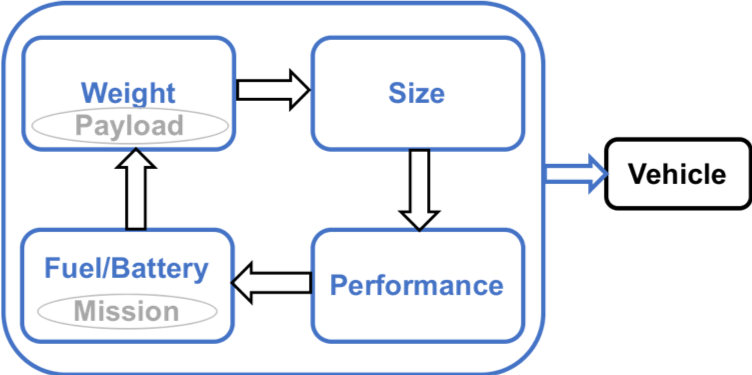
\includegraphics[width=0.65\textwidth]{images/iterate_loop.png}
\caption{Iterative sizing: the classical approach}
\label{fig:itsize1}
\end{center}
\end{figure}

\begin{figure}
\begin{center}
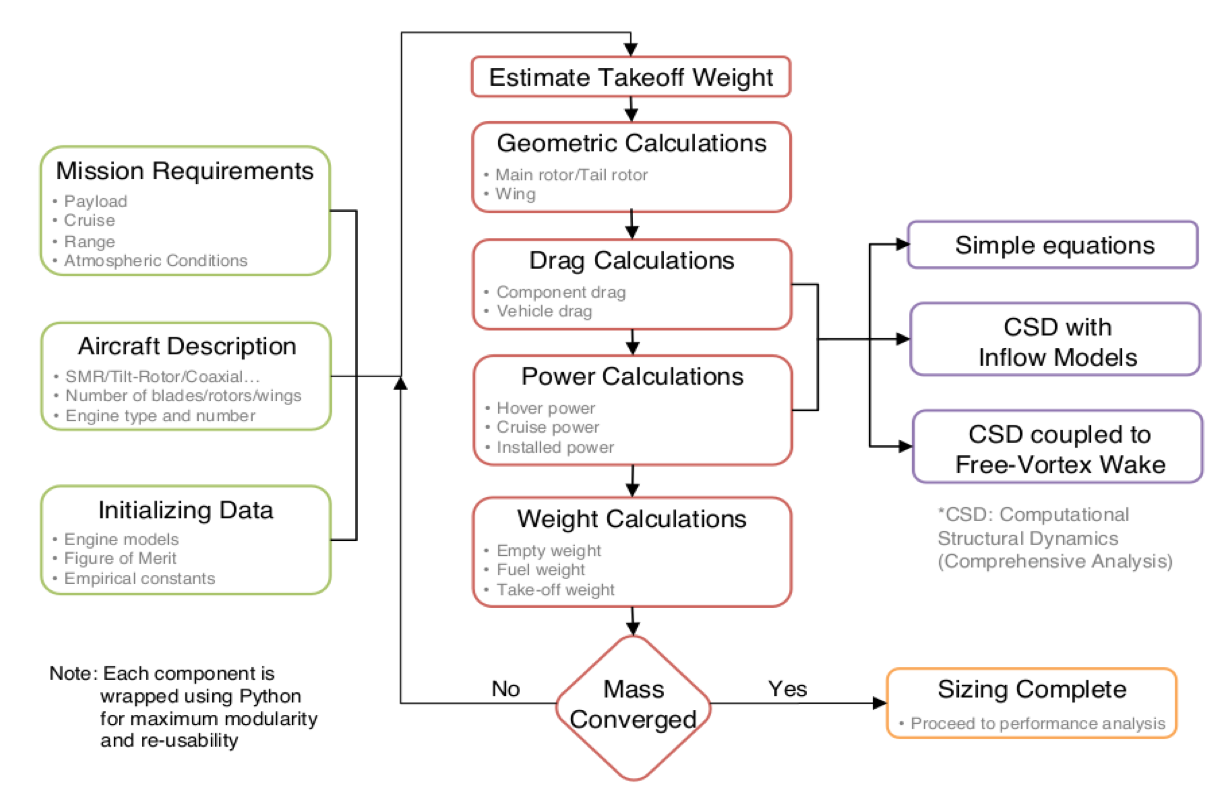
\includegraphics[width=\textwidth]{images/sizingloop.png}
\caption{Iterative sizing: detailed breakdown of operations}
\label{fig:itsize2}
\end{center}
\end{figure}

The \textbf{aircraft layout} is perhaps the most significant assumption required to initiate sizing. Figure~\ref{fig:evtols} shows a few candidate eVTOL configurations, with different permutations and combinations of rotor and wing technologies, as shown in Fig.~\ref{fig:evtol_types}. In \hydra, the constituent rotor and wing technologies are defined as primitive types. Based on user inputs, these technology combinations are superimposed in \hydra \spc to obtain the appropriate configuration. 

\begin{figure}
\begin{center}
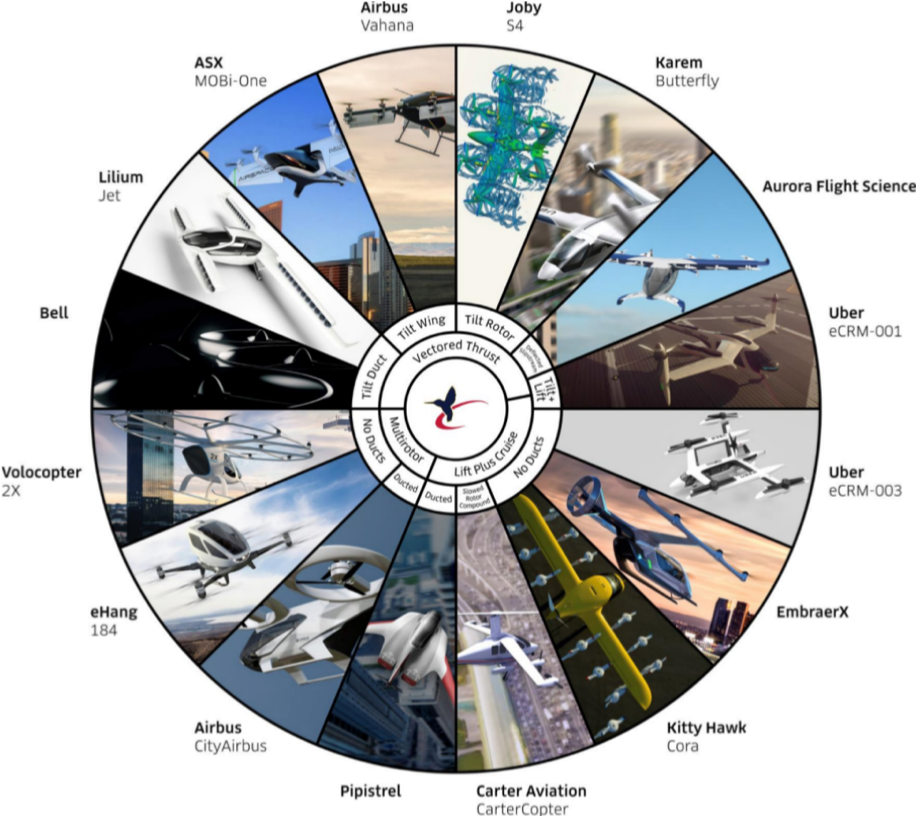
\includegraphics[width=0.75\textwidth]{images/evtols.png}
\caption{Variety in electric VTOL aircraft}
\label{fig:evtols}
\end{center}
\end{figure}

\begin{figure}
     \centering
     \begin{subfigure}
         \centering
         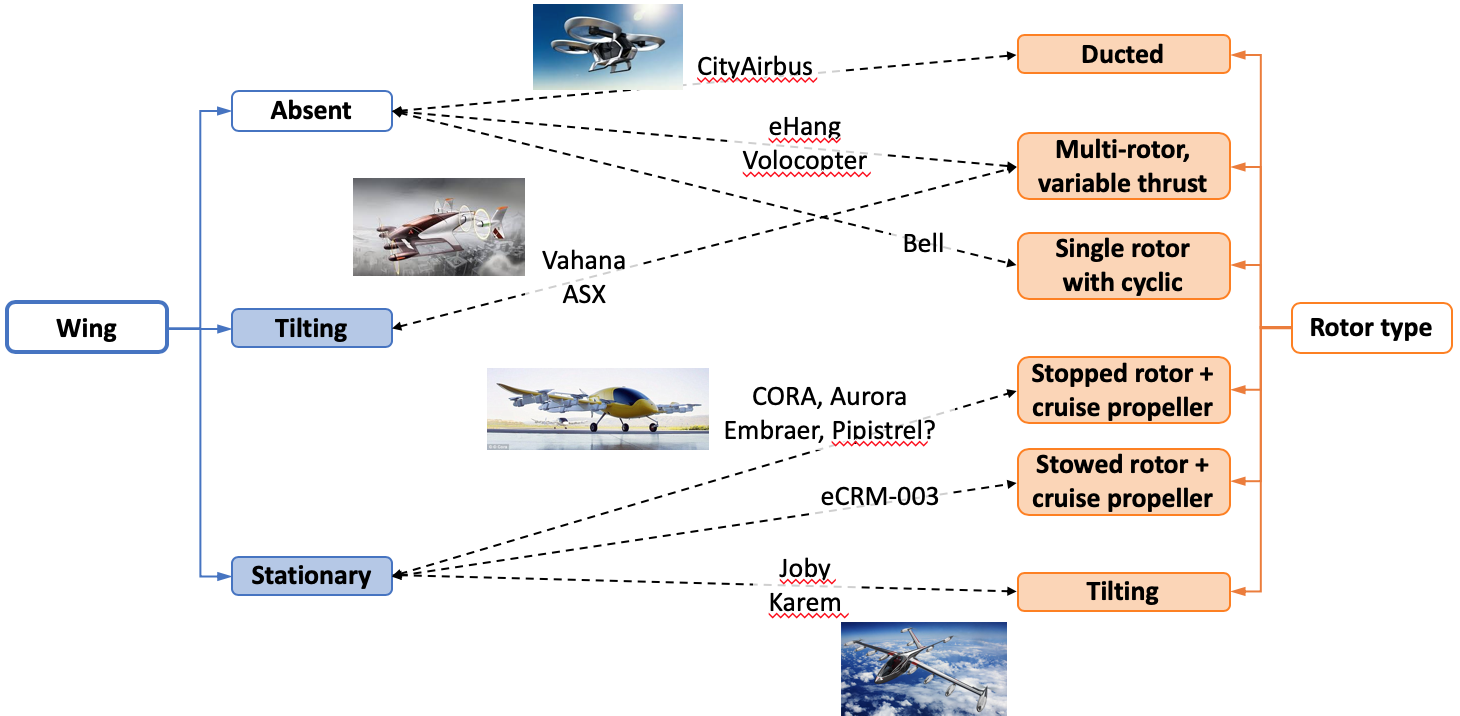
\includegraphics[width=\textwidth]{images/evtols1.png}
         \label{fig:evtols1}
     \end{subfigure}
     \hfill
     \begin{subfigure}
         \centering
         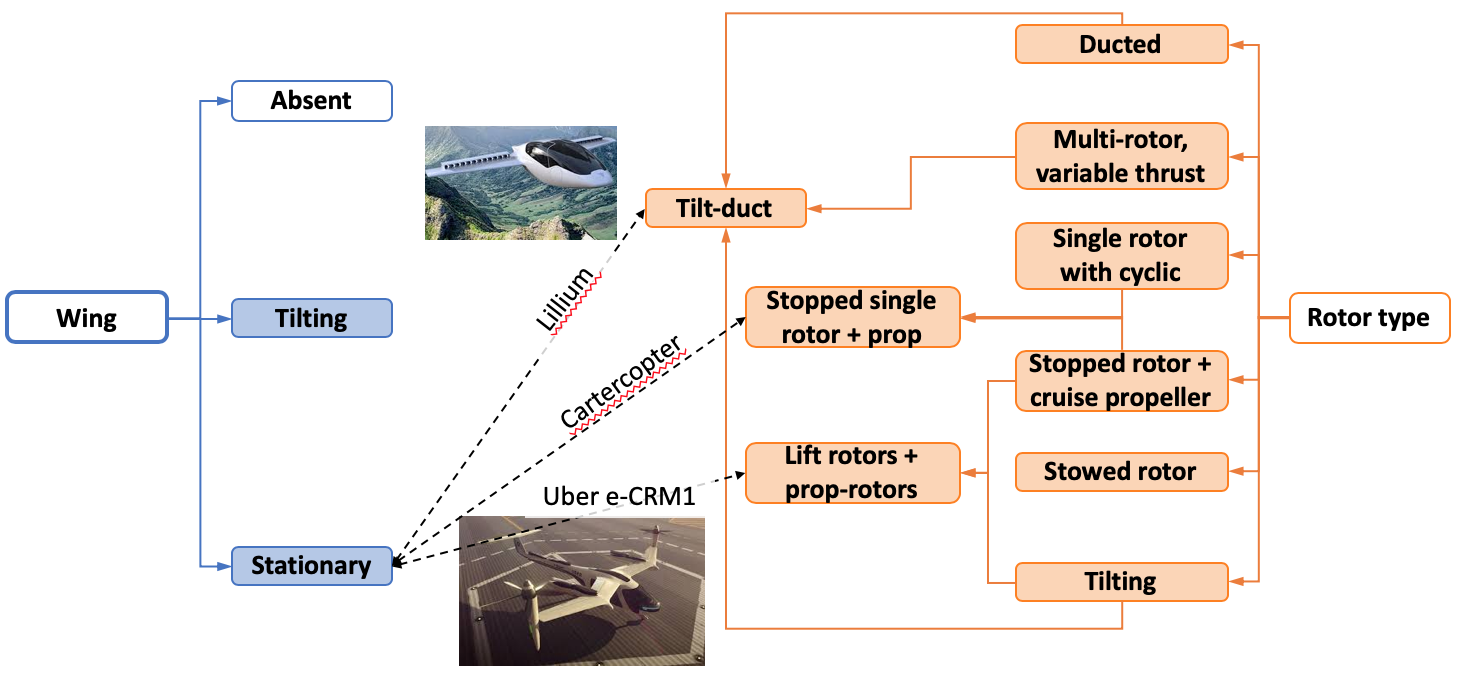
\includegraphics[width=\textwidth]{images/evtols2.png}
         \label{fig:evtols2}
     \end{subfigure}
        \caption{Assumbling eVTOLs from rotor and wing technologies}
        \label{fig:evtol_types}
\end{figure}

The \textbf{mission profile} is specified as a sequence of \textbf{hover} and \textbf{cruise} segments. Cruise segments are defined through a specified airspeed and distance/time, while hover segments are defined through duration. Climb and descent segments are defined as cruise segments with different start and end altitudes. An example mission profile is shown in Fig.~\ref{fig:mission}. 

\begin{figure}
\begin{center}
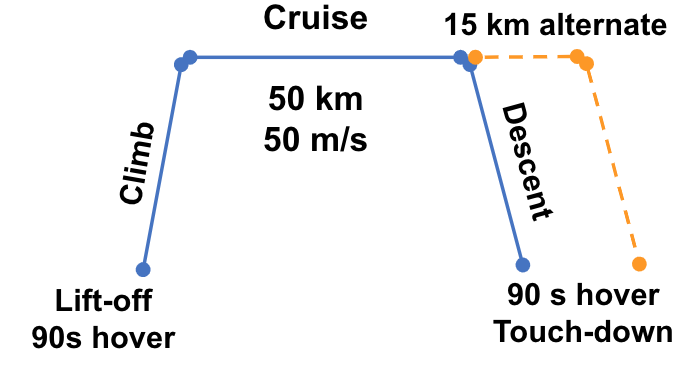
\includegraphics[width=0.75\textwidth]{images/mission.png}
\caption{An example mission profile}
\label{fig:mission}
\end{center}
\end{figure}

Finally, the \textbf{model calibration data} refers to calibration constants for parametric models of rotor performance, turboshaft engine performance, electric motors, fuselage drag vs. weight curve fits, and several other assumptions. Typically, up to 30 constants are required to calibrate different low-fidelity models accurately, defined in the \textbf{defaults.yaml} input file. In \hydra, several parametric models have been systematically replaced with higher-fidelity counterparts and so lift the specific assumptions made to arrive at those constants. \\
\textbf{Accelerated convergence} \\
The implementation of iterative sizing shown in Fig.~\ref{fig:itsize1} requires several iterations (up to 30) to converge take-off mass to the required tolerance. An alternate approach is implemented in \hydra, resulting in significantly faster convergence for no loss in accuracy. This accelerated convergence technique is shown in Fig.~\ref{fig:accel_conv}. 

In this method, the ``inner loop'' is executed in fixed take-off mass mode, and the constituent weight groups are evaluated. Finally, the remaining mass (take-off mass minus empty weight, minus energy storage) is assigned to payload mass, i.e., 

\begin{equation}
\textrm{m}_{\rm pay} \quad = \quad \textrm{M} \spc - \spc \textrm{m}_{\rm empty} \spc - \spc \textrm{m}_{\rm battery} \spc - \spc \textrm{m}_{\rm fuel}
\end{equation}

\begin{figure}
\begin{center}
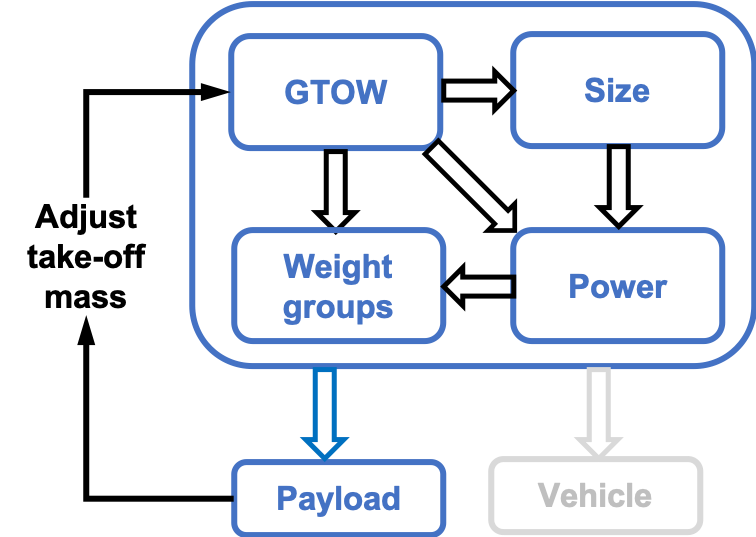
\includegraphics[width=0.5\textwidth]{images/accel_conv.png}
\caption{Accelerated convergence for iterative sizing}
\label{fig:accel_conv}
\end{center}
\end{figure}

Here, $M$ represents the take-off mass. Usually, mission profiles are specified together with the target payload m$_{\rm target}$. However, the ``inner loop'' described above runs once to calculate the payload mass m$_{\rm pay}$ for a given take-off mass $M$. Therefore, the take-off mass needs to be continuously adjusted to ensure that the ``calculated'' payload matches the target payload. One update scheme for the take-off mass (used in \hydra) is 
\begin{equation}
M_{i+1} \quad = \quad M_i - \frac{dM}{d\textrm{m}_{\rm pay}} (\textrm{m}_{\rm pay} - \textrm{m}_{\rm target})
\end{equation}
The slope $\frac{dM}{d\textrm{m}_{\rm pay}}$ is initially set to 3.0, and subsequently updated based on a finite-difference approximation as iterations proceed. This method usually converges in 3 -- 5 updates for take-off mass (vs. 30 iterations for the baseline technique), resulting in 5 -- 6 times faster convergence for no reduction in accuracy.

\subsubsection{Constrained optimziation}
The other technique that lends itself to VTOL conceptual sizing is constrained optimization. The primary advantage of this technique is that it allows for simultaneous minimization of a cost function (e.g. vehicle operating cost) while satisfying compatibility constraints (e.g., payload matching and landing footprint). If only sizing is required, the design variables are fed as prescribed inputs and compatibility constraints are specified as nonlinear algebraic constraints. The take-off weight is provided as a design variable and the payload is calculated as an output. The condition that the calculated payload (m$_{\rm pay}$) be at least the target mission payload (m$_{\rm target}$) is enforced as a nonlinear inequality constraint. 

In \hydra, two different optimizers are used for constrained minimization of the vehicle hourly operating cost: gradient-based optimization, and differential evolution. The constraints are landing footprint (based on wing span and fuselage length) and payload matching. For \textbf{concentual sizing}, gradient-based optimization requires an accurate initial condition to ensure that global minima (and not local minima) are identified at the end of optimization. In \hydra, the gradient-based optimizer is initialized from several starting conditions, each of which are obtained from a parametric sweep over the available high-level design variables. For \textbf{differential evolution}, compatibility constraints are implemented indirectly as a ``death penalty'' - an analog of exterior penalty functions. The cost function is increased by a large number (1e6) for designs that violate any of the user-specified constraints. Additionally, \hydra \spc is programmed to automatically add and remove design variables based on the number of rotor and wing groups in the vehicle. 

The optimizer in \hydra \spc is invoked after basic sizing over a limited parametric sweep is carried out. Both optimization techniques - gradient based and differential evolution - are used to minimize vehicle operating costs, and the resulting optimized designs are checked for uniqueness. These unique designs (obtained from optimization with different starting conditions) are ranked by operating cost, weight, battery/fuel or rated power based on a user-selected criterion. Further details are provided in the appropriate section later on in the documentation. 

\section{Drag models}

\subsection{Fuselage and empennage drag}
The fuselage is modeled as a slender body of revolution with its length set by user inputs, and an equivalent diameter based on body width and height (also set by the user). The procedure to calculate skin friction drag and base drag are identical to those documented in NASA CR-3083: \emph{ Rotary-Wing Aerodynamics: Volume II} by C.N. Keys. Similiarly, the approach for estimating the drag of horizontal and vertical tail surfaces, as documented in NASA CR-3083, is implemented in \hydra.

\subsection{Edgewise rotor hub drag}
The flat-plate area of each edgewise rotor hub is estimated based on a modified procedure outlined in NASA CR-3083, as follows:
\begin{equation}
f_{\rm hub} \quad = \quad 1.2 R^2 (0.0006 + 0.00222 N_{\rm b})
\end{equation}

\subsection{Spinner drag}

The spinner is assumed to be a rotating body with a hemispherical nose and blunt base. As shown in Fig.~\ref{fig:fus_drag}, the drag coefficient of such a shape is 0.2 (referenced to cross-sectional area $\pi d^2/4$), for a length-to-diameter ratio of 2.5. For the calculations presented in this paper, a drag coefficient of 0.36 is assumed, to account for additional blockage from the airframe, vertical fins and interference effects. The radius of the spinner is 15\% of the rotor radius. 

\begin{figure}
\begin{center}
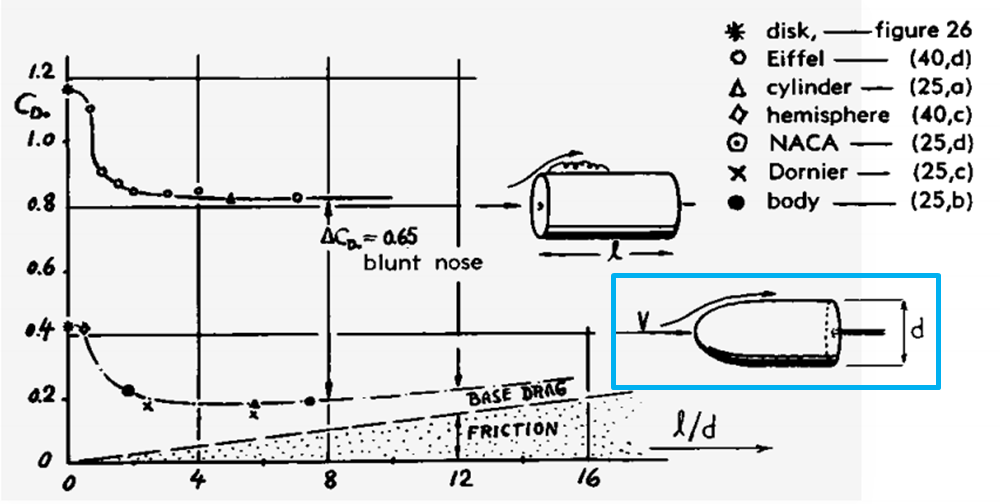
\includegraphics[width=\textwidth]{images/fus_drag.png}
\caption{Spinner nose cone:drag coefficient, from \emph{Fluid Dynamic Drag, Hoerner}}
\label{fig:fus_drag}
\end{center}
\end{figure}

\subsection{Momentum drag for engine air intakes}
For turboshaft engines operating at cruise speeds above 160 knots, the additional momentum drag is 0.3 ft$^2$ per intake.

\subsection{Landing gear drag}
The drag of landing gear is modeled with a parametric representation (obtained from NASA CR-3083) as follows:
\begin{equation}
\log_e f_{\rm LG} \quad = \quad y_0 + m \log_e(0.001 W)
\end{equation}

Here, $f_{\rm LG}$ is in square feet, and $W$ is in lbs. The constants $y_0$ and $m$ are set based on the type of landing gear. 
\begin{enumerate}
\item \textbf{Retracted gear}: $f_{\rm LG}$ = 0
\item \textbf{Wheeled gear}: $y_0$ = 0.5755. The slope $m$ = 0.443  for W $\geq$ 1000 lb, and zero for W $\leq$ 1000 lb.
\item \textbf{Skid gear}:  $y_0$ =-0.11626. The slope $m$ = 0.4979  for W $\geq$ 1000 lb, and zero for W $\leq$ 1000 lb.
\end{enumerate}

\subsection{Cooling drag}
The cooling systems required to regulate engine temperatures creates additional drag, which is estimated using a parametric model given in NASA CR-3083.
\begin{equation}
f_{\rm cool} ({\rm ft}^2)\quad = \quad 10^{-4} P_{\rm ins} (hp)
\end{equation}

\subsection{Mast fairing drag for coaxial rotors}
The fairing for the exposed length of the rotor shaft between the upper and lower rotors of a coaxial system incurs an additional drag penalty, given by 
\begin{equation}
f_{\rm mast} ({\rm ft}^2)\quad = \quad 0.0322 R^2
\end{equation}

\subsection{Protrusion drag}
The drag of protrusions is modeled as an additional 10\% of the accumulated parasitic drag of all wetted surfaces.

\section{Rotor and Wing Performance Models}

\subsection{Rotor performance model}

Two performance models are used to calculate rotor power required in hover and axial flight. The first model is based on momentum theory, and the second model is based on blade element momentum theory. 

\subsubsection{Momentum Theory}
For momentum theory-based predictions, rotor power is calculated based on assumed aerodynamic efficiency factors in hover and cruise. Imperial units (foot, pounds of force and horsepower) are assumed for these expressions. In hover, rotor power is given by 
\begin{equation}
P_{\rm hover} (hp) \quad = \quad \frac{T_R^{1.5}}{550 \sqrt{2 \rho A} \textrm{ FM}}
\end{equation}
Here, $T$ is the thrust required in hover from each rotor, and is calculated assuming the segment weight is equally divided between all rotors. A vertical download factor (configuration-dependent) is included in the estimation of rotor thrust. The rotor disk area is $A$ (ft$^2$), $\rho$ is the ambient air density (slug/ft$^3$) and FM is the rotor figure of merit in hover. 

In cruise, the power required by each rotor when operating in axial flight is 
\begin{equation}
P_{\rm cruise} (hp) \quad = \quad \frac{D}{N_{_\textrm{R}} } \frac{V_{\infty}}{550 \eta_{\rm p}}
\end{equation}

Here, $D$ is the total vehicle drag in lbs when operating at a forward flight speed of $V_{\infty}$ ft/s, which is overcome by each of the N$_{_\textrm{R}}$ rotors operating at a propeller efficiency of $\eta_{\rm p}$. 

%The assumed figure of merit $FM$ and propeller efficiency in cruise $\eta_{\rm p}$ are 0.7 and 0.8, respectively.

\subsubsection{Blade Element Momentum Theory (BEMT)}
Certain configurations like the tilt-rotor or tilt-wing fly such that the rotors operate predominantly in axial flight. Therefore, the Blade Element Momentum Theory (BEMT) is used as a higher-fidelity replacement for momentum theory-based predictions. Though BEMT can resolve finer details like angle of attack variations along the span, it requires detailed inputs, namely airfoil tables and distribution of blade chord and twist along the span. These details are populated as described below.

The rotor is assumed to be constructed from multiple user-specified airfoils. The lift and drag characteristics for each airfoil may be Reynolds-tabulated or mach-tabulated. Several combinations of blade chord and twist distribution are generated assuming linear taper and bilinear twist. The design variables for blade geometry are:
\begin{enumerate}
\item Blade taper ratio (1:1, 2:1 and 3:1)
\item Blade bilinear twist junction (30\% -- 70\% span)
\item Twist at bilinear junction (-5 deg to -20 deg)
\item Twist at tip (-5 deg to -35 deg)
\end{enumerate}
The rotor RPM in cruise (specified as a fraction of hover RPM) is added as a sizing variable. The BEMT analysis calculates the rotor power required for a given thrust, for all mission segments, exploring a parameter space of 360 designs (combinations of blade twist and taper distribution). The rotor geometry for minimum energy consumption over the mission is identified from the parametric sweep, and the aerodynamic efficiencies (figure of merit $FM$ in hover and propeller efficiency $\eta_{\rm p}$ in cruise) are calculated for each mission segment. 

Minimizing the energy required at the rotor ensures reduced fuel consumption, but not necessarily a good overall design. A cruise-dominated mission results in a prop-rotor with a potentially degraded hover figure of merit while achieving good aerodynamic cruise efficiency. Therefore, installed power (and therefore, engine and transmission weights) may increase, resulting in a lower payload fraction. To prevent unchecked increases in powerplant weights, another condition is introduced in the BEMT analysis: designs are considered ``valid" if the hover figure of merit is greater than a user-specified threshold (e.g., 0.72), and only these valid designs are ranked to determine the ``best'' rotor efficiencies.

When BEMT is included in the sizing iterations, sizing proceeds in 3 steps:
\begin{enumerate}
\item Perform sizing with momentum theory and assumed efficiency factors in hover and cruise ($FM$=0.75, $\eta_{\rm p}$=0.82)
\item If the design satisfies all constraints, perform BEMT analysis to calculate aerodynamic efficiencies for each segment based on thrust requirements; extract hover or cruise efficiencies (FM, $\eta_{\rm p}$).
\item Perform sizing with momentum theory, using the calculated rotor aerodynamic efficiencies obtained in Step 2.
\end{enumerate}

%When BEMT is included in sizing, the rotor performance calculations are the bottlenecks for computational efficiency; 8 designs can be sized in one second, compared to 50 designs per second when using momentum theory with the FEA-based airframe weight model.

\begin{figure}
\centering    
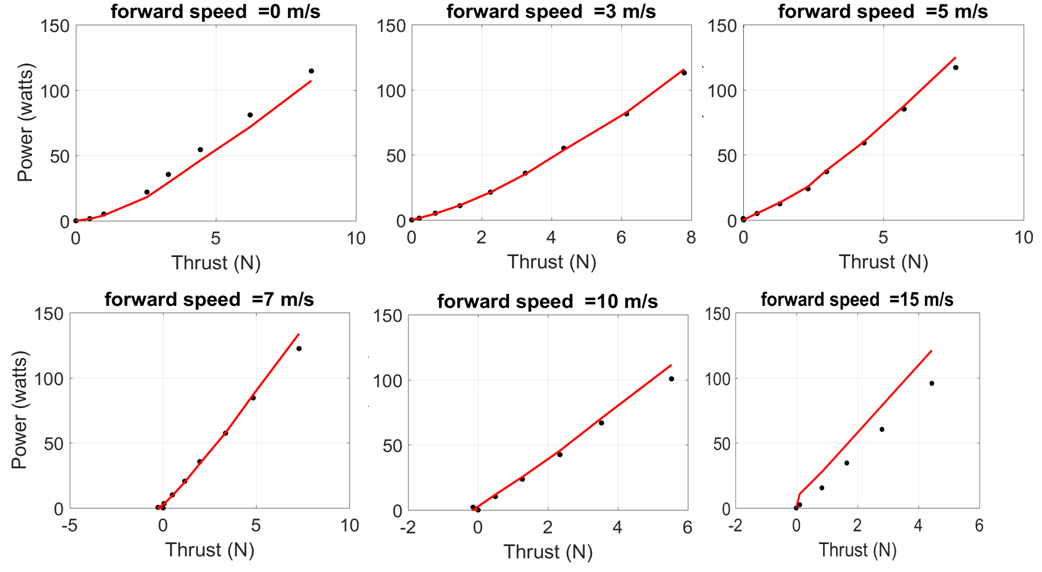
\includegraphics[width=\textwidth]{images/bemt_validation.png}
\vspace{-1cm}
\caption{Comparison of BEMT predictions to experiments}
\label{fig:bemt}
\end{figure}

Figure~\ref{fig:bemt} shows the comparison of thrust and power obtained from BEMT predictions with airfoil tables vs. sub-scale experiments for a variable-pitch and variable-RPM sub-scale prop-rotor. Good predictions were obtained at various cruise speeds ranging from 3 m/s to 15 m/s. For these cases, BEMT was found to be sufficient for accurate performance predictions. %The rotor geometry and details of the experiment were obtained from Ref.~\citenum{Phillips16}.

\subsection{Wing performance model}
The drag coefficient of a fixed wing is given by 
\begin{equation}
C_D \quad = \quad C_{Do} \spc + \spc \frac{1}{\pi AR e} C_L^2 
\end{equation}
The lift coefficient $C_L$ and aspect ratio $AR$ are sizing design variables. The profile drag coefficient $C_{Do}$ is an assumed value, usually 0.014 (including protrusions and interference). The Oswald efficiency $e$ is calculated as %using the methodology of Kroo, summarized by Nita and Scholz as follows:
\begin{align*}
e \quad &= \quad \left(Q + P \pi AR \right)^{-1}  \\
P \quad &= \quad 0.38 \times 0.02 \\
Q \quad &= \quad \frac{1.01}{s} \\ 
s \quad &= \quad 1 \spc - \spc 2 \left(\frac{d_{\rm fus}}{b_{\rm wing}}\right)^2
\end{align*}
The parameters are $d_{\rm fus}$ = equivalent fuselage diameter, and $b_{\rm wing}$ = wing span.
\pagebreak
\section{Weight models}
There are three main contributors to vehicle take-off mass:
\begin{enumerate}
\item {\bf Energy storage} - battery and/or fuel weight. This component may be traded-off against payload for mission flexibility, depending on available volume. 
\item {\bf Empty weight} - this weight group represents the airframe, wings, rotors, engines, transmission, motors, seats, avionics and other non-removable systems.
\item {\bf Payload} - usually specified with the mission definition.
\end{enumerate}

\subsection{Engines, fuel and batteries}
Though engines strictly belong in the empty weight category, the calculation of fuel weights are inextricably linked to the evaluation of engine performance and engine weights. Therefore, engine models are described in this section. 

\subsubsection{Engines}
\hydra \spc has built-in models for fuel-burning engines of two types: gas turbine engines, and reciprocating engines (piston engines and aero-diesel engines). \\
\textbf{Turboshaft engines} \\
Based on statistical data for various production engines, a trend line was fitted with good accuracy ($R^2 = 0.92$) for the variation of engine weight W$_{\rm engine}$ (lb) with installed power P$_{\rm ins}$ (hp). The fitted engine weight model is given by
\begin{equation}
\label{eqn:turbowt}
W_{\rm engine}\spc (\textrm{lb}) \quad = \quad 7.3874 \textrm{ P}_{\rm ins}^{0.552}
\end{equation}
Another fit is shown in Fig.~\ref{fig:turboshaft}, in SI units with engines manufactured over the last fifty years.

The variation of engine Specific Fuel Consumption (SFC) at peak efficiency with installed power is 
\begin{equation}
\textrm{sfc}_{_{\rm base}} \spc (\textrm{lb/hp-hr}) \quad = \quad 1.549 \textrm{ P}_{\rm ins}^{-0.161}
\end{equation}
Engines operating at sub-optimal conditions (i.e. at power settings lower than design power output) suffer from higher specific fuel consumption. This effect is modeled using a power law as 
\begin{equation}
\label{eqn:sfcpower}
\textrm{sfc} \quad = \quad \textrm{sfc}_{_{\rm base}} \left(\frac{\textrm{P}_{\rm req}}{\textrm{P}_{\rm ins}}\right)^{-0.256}
\end{equation}
Here, P$_{\rm req}$ is the power output required from the engine to produce a thrust $T$ during a mission segment. Finally, the variation of available power (relative to installed power) with ambient temperature and pressure is given by 
\begin{equation}
\textrm{P}_{\rm avail} \quad = \quad \textrm{P}_{\rm ins} \spc [1 - K_T (\theta-1)] \spc [1 + K_D (\delta-1)]
\end{equation}
The terms $\theta$ and $\delta$ are ratios of ambient temperature and ambient pressure to their corresponding values at mean sea level (ISA). The constants $K_T$ and $K_D$ are obtained from curve fits of detailed engine performance curves. \\
\begin{figure}
\begin{center}
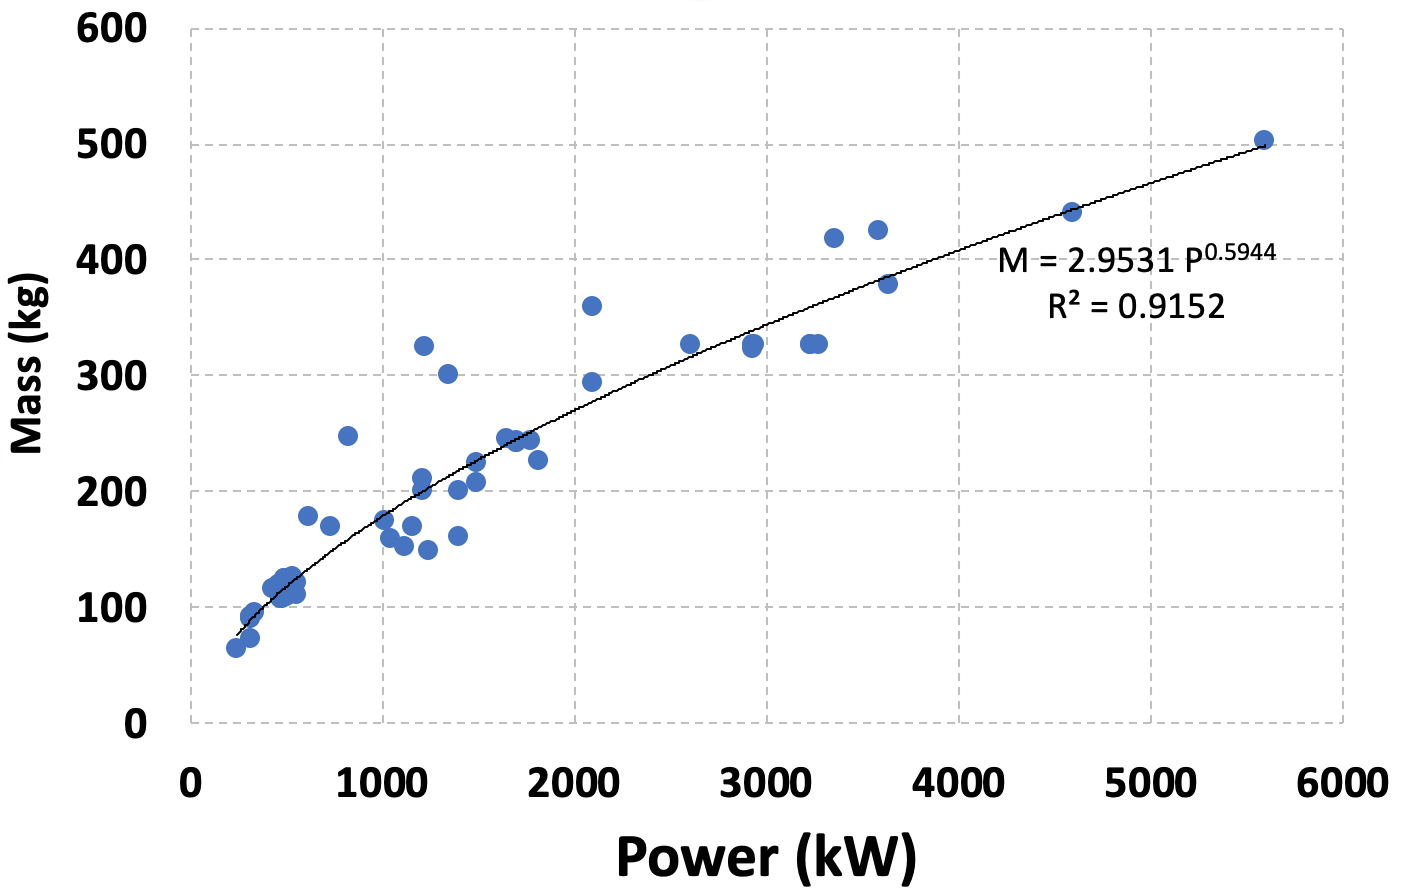
\includegraphics[width=0.75\textwidth]{images/turboshaft.png}
\vspace{-0.1cm}
\caption{Statistics: turboshaft engine mass vs. installed power}
\label{fig:turboshaft}
\end{center}
\end{figure}
\textbf{Piston engines} \\
The treatment of piston engine weights is similar to that followed for turboshaft engines. The variation of engine weight with installed power is given by 

\begin{equation}
\label{eqn:pistonwt}
W_{\rm engine}\spc (\textrm{lb}) \spc = \spc 2.367 \textrm{ P}_{\rm ins}\textrm{ (hp)} ^ {0.916} \quad 35 \leq \textrm{ P}_{\rm ins}\textrm{ (hp)} \leq 1000
\end{equation}
Another fit is shown in Fig.~\ref{fig:piston}, in SI units with a larger sample size, including less efficient engines. The variation of engine SFC at its peak efficiency is 
\begin{align*}
\textrm{sfc}_{_{\rm base}} (\textrm{lb/hp-hr}) \spc = &\spc 0.42, \spc \textrm{ P}_{\rm ins} \textrm{ (hp)} \leq 4 \\
=&\spc 0.594 - 0.0046 \textrm{ P}_{\rm ins} \textrm{ (hp)}, \spc 4 \leq \textrm{ P}_{\rm ins} \leq 56 \\
=&\spc 0.52 \textrm{ P}_{\rm ins} \textrm{ (hp)}^{-0.0972}, \spc 56 \leq \textrm{ P}_{\rm ins} \leq 1000
\end{align*}

\begin{figure}
\begin{center}
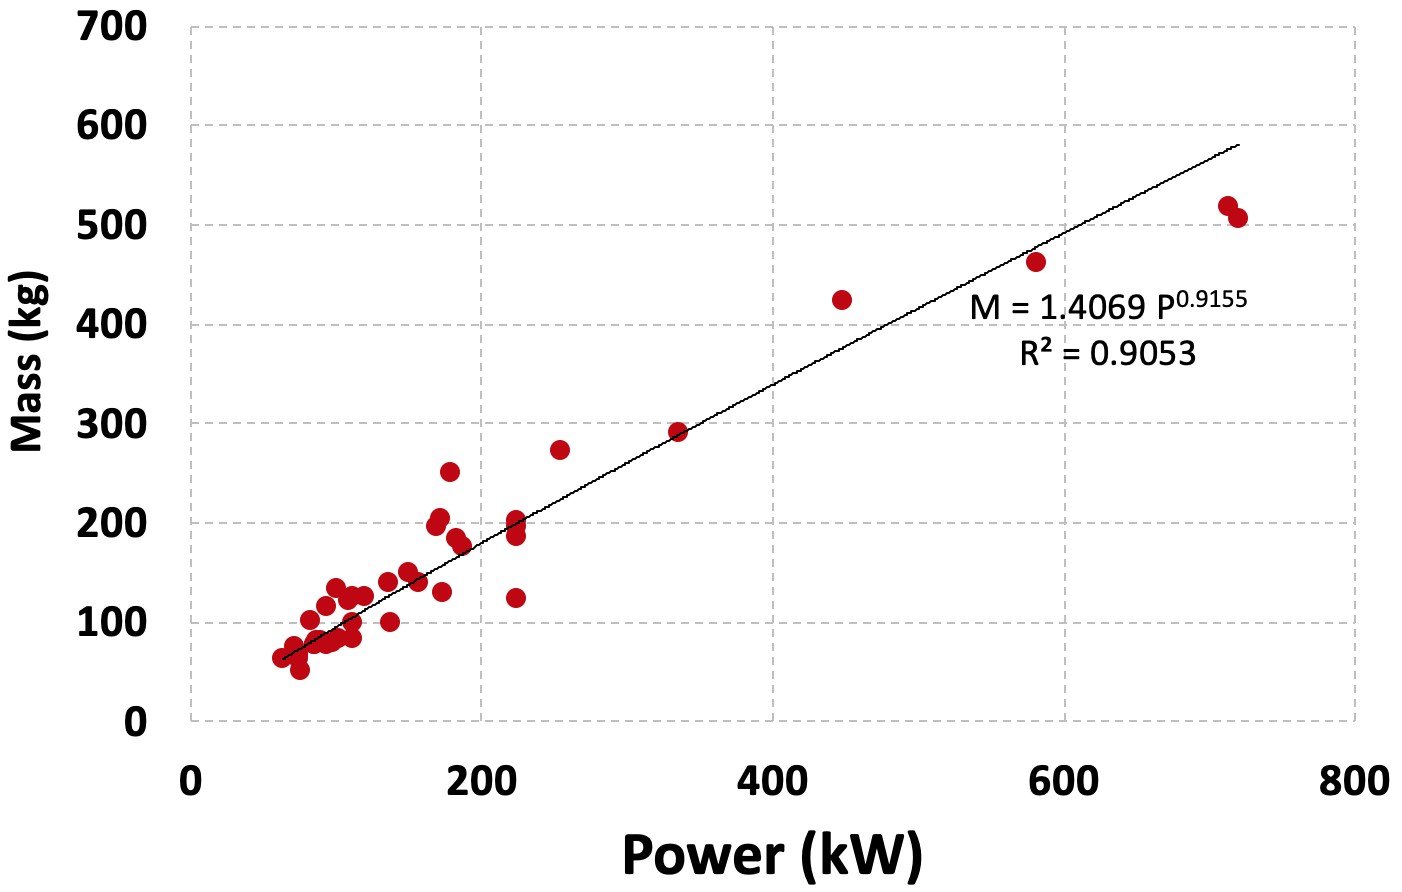
\includegraphics[width=0.75\textwidth]{images/piston.png}
\vspace{-0.1cm}
\caption{Statistics: reciprocating engine mass vs. installed power}
\label{fig:piston}
\end{center}
\end{figure}

%Increases in engine SFC based on the operating condition are modeled similar to efficiency degradation of the turboshaft engine as given in Eqn.~\ref{eqn:sfcpower}.
\subsubsection{Fuel, tank and fuel handling systems}
After calculating the engine power required, the mission profile (flight segment duration) is used with engine power requirement and SFC estimates to calculate the fuel weight as 
\begin{equation}
m_{\rm fuel} \quad = \quad \mathlarger{\mathlarger{\Sigma}}_{i=1}^{\rm N_{\rm SEG}} \spc sfc(i) \spc P_{\rm eng}(i) \spc + \spc m_{\rm unusable}
\end{equation}
An average density of 6.7 lb/gal is used for both turbine engine fuel and aviation gasoline. The fuel tank and plumbing mass is estimated from fuel volume using AFDD models as 
\begin{equation}
   W_{\rm tank} \quad = \quad 0.4341 \spc V_{\rm tank}^{0.7717} \spc N_{\rm tank}^{0.5897}  \spc f_{\rm cw} \spc  f_{\rm bt}^{1.9491}
\end{equation}
The terms used in the equations are \\
V$_{\rm tank}$ is the tank volume in U.S. gallons (1 gal = 3.7.8 liters)\\
N$_{\rm tank}$ is the number of internal tanks \\
$f_{\rm cw}$ is the crashworthiness mark-up factor, usually 1.31 \\
$f_{\rm bt}$ is the ballistic survivability mark-up factor (1.2 for military, 1.0 for civilian) 

The weight of plumbing systems used for regulating fuel flow from tanks to engines is modeled as follows:
\begin{align*}
k0_{\rm plumb} \quad &= \quad \textrm{max}(0.022 M, 120) \\
k1_{\rm plumb} \quad &= \quad 0.025 k0 \\
W_{\rm plumb} \quad &= \quad k0_{\rm plumb} + k1_{\rm plumb} (0.01*N_{\rm tank} + 0.06*N_{\rm engine}) \spc \dot{V}^{0.866}
\end{align*}
$\dot{V}$ is the peak fuel flow rate to the powerplant in lb/hr and the plumbing system weight is in pounds. $M$ is the take-off mass in kg - the mixing of units and conventions is a result of AFDD models being specified in FPS units, while \hydra \spc is implemented in SI units. 

For small-scale powerplants, the trendlines predict an over-estimate of fuel handling system weight. To handle these special cases, a maximum limiter is placed on the fuel system weights, with the limit set to 50\% of fuel weight. 

\subsubsection{Battery models}
Battery weights are accurately represented using a very simple statistical model. Figure~\ref{fig:smallbattery} shows the variation of battery weight with rated energy capacity for commercially available small-scale batteries, where each data point represents a manufactured unit. Arguably, a battery density of 158 W-hr/kg is quite low and improvements can be made;  this ``conservative'' design is typical of commercially available battery packs including the safety casing. 

\begin{figure}
\begin{center}
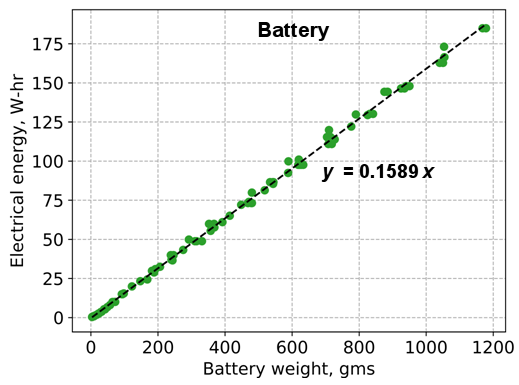
\includegraphics[width=0.75\textwidth]{images/battery.png}
\vspace{-0.1cm}
\caption{Small-scale batteries: weight statistics}
\label{fig:smallbattery}
\end{center}
\end{figure}

For full-scale platforms used in commercial operations, several conservative assumptions are used to incorporate various margins in sizing the battery. 
\begin{enumerate}
\item The minimum depth of discharge is 7.5\% of total energy capacity
\item The maximum state of charge near end of life for the battery is 80\%, i.e., after cycling, the usable battery capacity is at most 80\% of the rated energy. Thus, the effective usable energy for battery sizing is \textbf{72.5\% of the rated capacity}. 
\item The average discharge efficiency of the battery reduces by 4\% for every unit increase in average C-rating. 
\item A specific energy of 240 Wh/kg is used to estimate the mass of the cells.
\item A pack integration factor of 0.75 (defined as battery mass to cell mass) is used to estimate the weight of battery management systems and casing.
\item A curve fit of temperature rise vs. C-rating (obtained from experimental data) is used to track the rise of cell temperature over the mission duration. A maximum  limit of of 70$^o$C is used to iteratively add cells until thermal limits are satisfied.
\end{enumerate}

\subsubsection{Electric motor weights}
Though electric motor weights are strictly driven by peak torque requirements, the data correlation between weight and peak rated power is also very good as shown in Fig.~\ref{fig:smallmotor}. For small-scale motors, the speed controller is sized based on the current drawn by the system assuming a 12 Volt source. The masses of several large-scale motors with controllers are plotted against rated power in Fig.~\ref{fig:dcmotor}. Motor + speed controller efficiencies range from 85\% to 92\% depending on the design point and operating RPM range. Motor and speed controller weights are estimated as 
\begin{align*}
W_{\rm motor} (lb) \spc = & \spc 0.74 \textrm{ P} \qquad \qquad \qquad \textrm{P} \leq 13.4 \textrm{ hp} \\
W_{_\textrm{ESC}} (lb) \spc = & \spc 1.047 \textrm{ P} \qquad \quad \qquad \textrm{      P} \leq 13.4 \textrm{ hp}\\
W_{\rm motor} + W_{_\textrm{ESC}} (lb) \spc = & \spc 1.489  \textrm{ P}^{0.783} \quad 13.4 \textrm{ hp} < \textrm{P} \leq 350 \textrm{ hp}
\end{align*}

\begin{figure}
\begin{center}
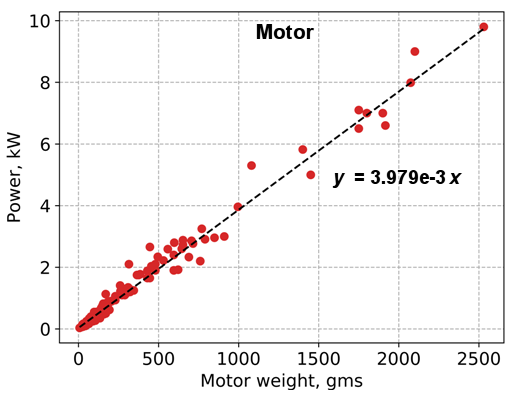
\includegraphics[width=0.75\textwidth]{images/motor.png}
\vspace{-0.1cm}
\caption{Statistics: weight of small BLDC motors}
\label{fig:smallmotor}
\end{center}
\end{figure}

\begin{figure}
\begin{center}
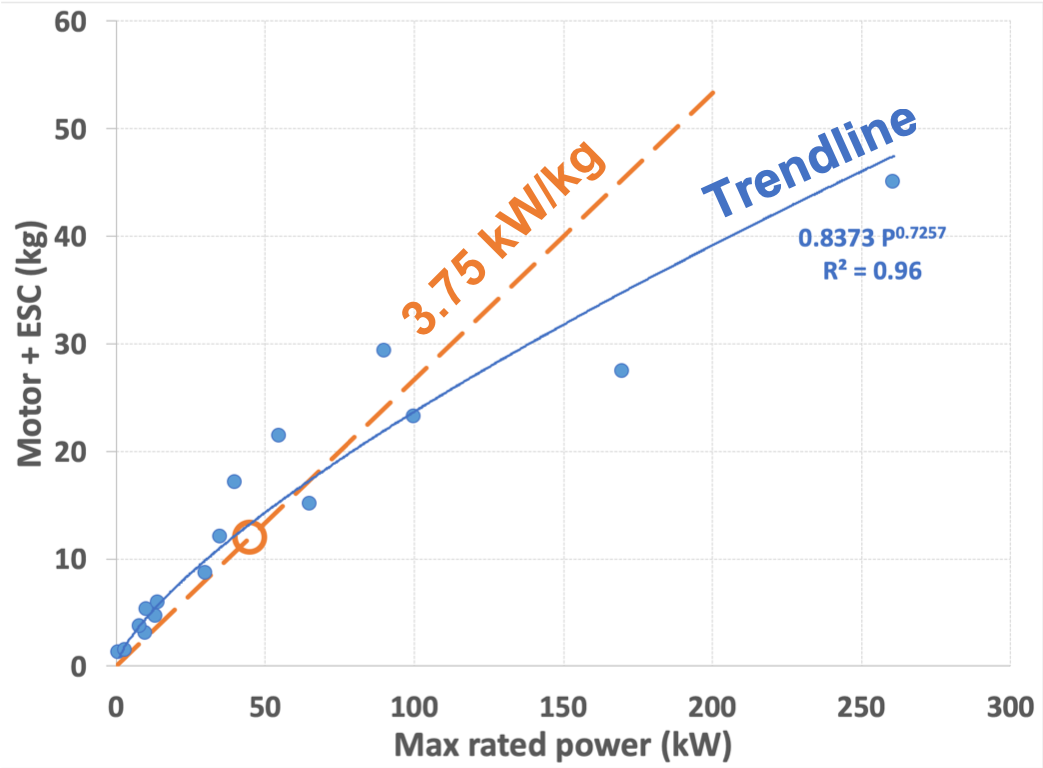
\includegraphics[width=0.75\textwidth]{images/dcmotor.png}
\vspace{-0.1cm}
\caption{Statistics: large-scale DC motor + controller mass vs. installed power. Manufacturing technology in 2018 can achieve 3.75 kW/kg of power density.}
\label{fig:dcmotor}
\end{center}
\end{figure}


 %For prop-rotors, the hover point is usually chosen as the operating condition for maximum efficiency (92\%), with the cruise point being chosen for lower motor efficiencies. 

\subsection{Electric Transmissions}
Generators for electric transmissions are sized in a manner identical to electric drive motors. The components of an electric transmission are shown in Fig.~\ref{fig:eltrans}.

\begin{figure}
\begin{center}
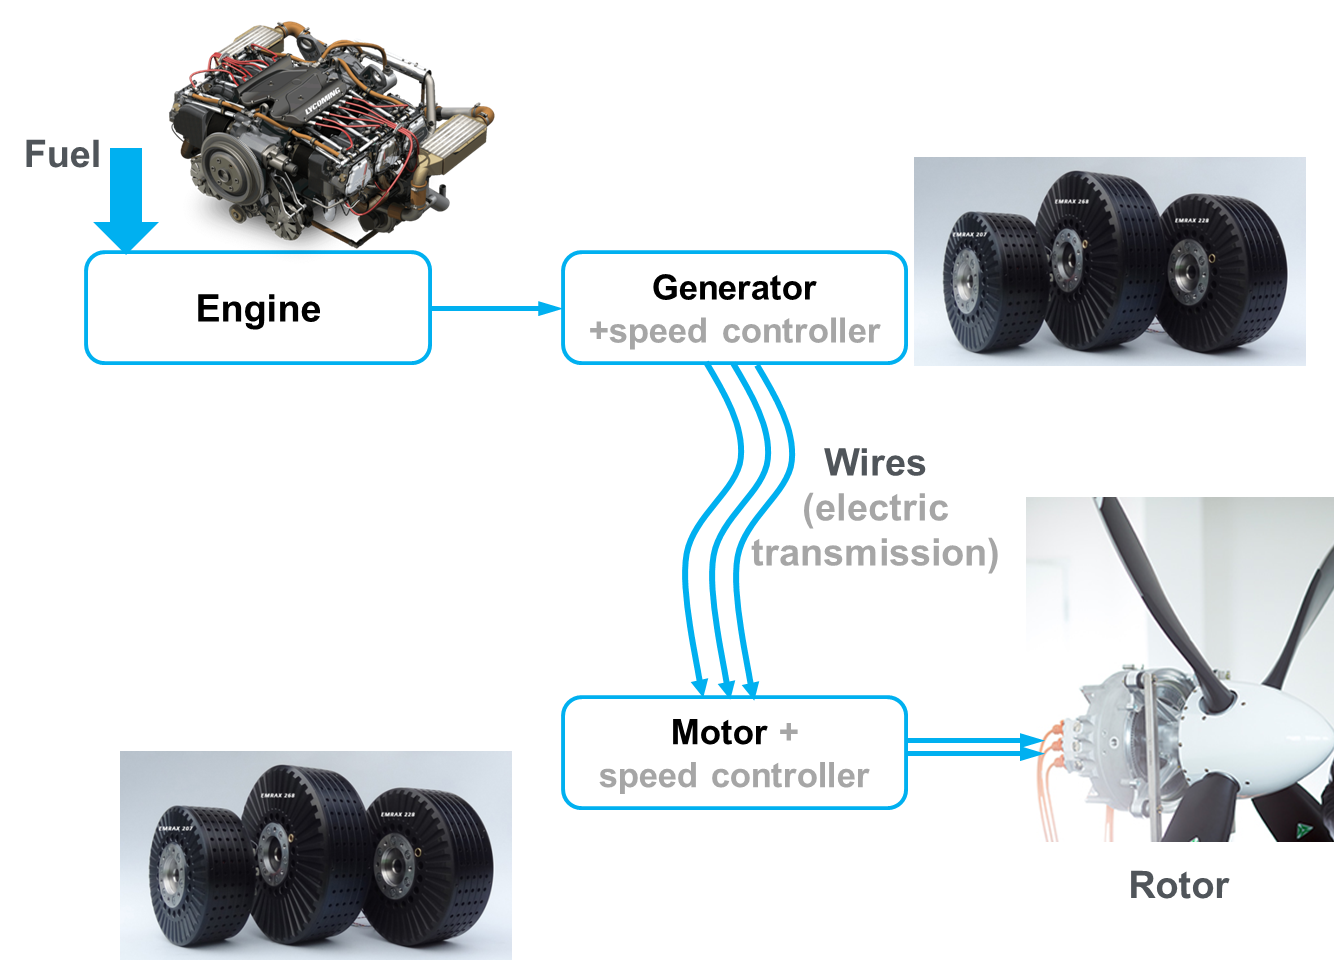
\includegraphics[width=0.75\textwidth]{images/eltrans.png}
\vspace{-0.1cm}
\caption{Turbine-generator hybrid powerplant for electric motor. 98\% wire transmission efficiency, 92\% generator efficiency}
\label{fig:eltrans}
\end{center}
\end{figure}

The advantage of this hybrid system is that a mechanical transmission is not required for power transmission to the rotors; further the hybrid system can serve as a long-range drop-in upgrade for short-range battery-powered variants. The disadvantage of a turboshaft-electric hybrid system is that each additional component introduces additional points of failure. Adding redundancy and fail-safe architectures can incur a significant empty weight penalty.

\subsection{Wire weights}
Two types of wires are considered in the sizing analysis: power cables and signal wires. The weights of electrical power cables are estimated from the vehicle rotor layout using a wire mass per unit length per unit power of 0.0057 kg/kW/m. Signal wires are calculated using a linear mass density of 0.17 kg/m and a knowledge of the rotor layout, together with an estimate of channel counts. Based on user inputs, doubly/triply redundant power cables and signal wires are automatically added to the appropriate weight groups for estimating vehicle empty mass.

At full-scale, a key driver of vehicle weight is the rotor design parameter set (tip speed, solidity, disk loading/radius, first rotating flap frequency). One such empirical parameter is the flap natural frequency. In the legacy approach for estimating rotor blade weight, the designer had to prescribe this parameter to perform sizing. However, underlying data for the flap frequency is restricted to articulated and hingeless rotors, and plentiful data is not available for stiffer rotors ($\nu_\beta \geq$ 1.08/rev). For small-scale VTOL with very stiff rotor systems ($\nu_\beta$ $\geq$ 1.4/rev), extrapolation of the trend line beyond the range of available data for $\nu_\beta$ may yield erroneous estimates for rotor blade weight. For eVTOLs, a physics-based approach is implemented and used in \hydra.

\subsection{Physics based model for rotor blades}

\begin{figure}
\begin{center}
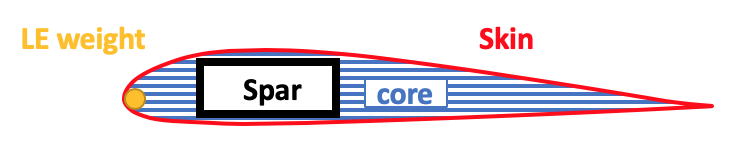
\includegraphics[width=0.75\textwidth]{images/cross_section.png}
\vspace{-0.1cm}
\caption{Blade cross-section}
\label{fig:cross_section}
\end{center}
\end{figure}

A schematic of the rotor airfoil is shown in Fig.~\ref{fig:cross_section}. The cross-section consists of two categories of materials: non-structural masses, and load-bearing components. The non-structural masses are:
\begin{enumerate}
\item Paint: 0.15 mm thickness, density 1800 kg/cu.m, applied on surface
\item Glue: 0.25 mm thickness, density 1800 kg/cu.m, applied on skin, shear webs
\item Core: density of 52 kg/cu.m, encompasses cross-section area of 0.49 $\left(\frac{t}{c}\right) c$
\item Leading edge protection: 1.14mm thickness, density 8900 kg/cu.m, from leading edge to 25\% chord on upper and lower surfaces.
\end{enumerate}
Here, $\left(\frac{t}{c}\right)$ is the airfoil thickness-to-chord ratio, usually 0.1 to 0.12 and $c$ is the blade airfoil chord. For the paint and glue, the chordwise location of the component center of gravity is 0.5$c$. For the leading edge protection strip and core, the component chordwise center of gravity locations are 12.5\% chord and 57\% chord, respectively. 

\subsubsection{Skin sizing}
The skin is sized to withstand a total torsion moment equivalent to an airfoil $c_m$=0.2 at the maximum rated rotor speed. The total root pitching moment in hover is 
\begin{equation*}
M_x \quad = \quad \frac{1}{6} \rho V_{\rm TIP}^2 c^2 c_m R 
\end{equation*}
The skin thickness is given by 
\begin{equation*}
t_{\rm skin} \quad = \quad \frac{n M_x}{2 A_{\rm cs} \tau_{\rm skin}}
\end{equation*}
Here, $A_{\rm cs}$ is the cross-section area of the airfoil, and $\tau_{\rm skin}$ is the maximum allowable shear stress in the skin. The factor $n$ accounts for additional overload and safety factors to account for for contingency conditions and fatigue margins. 

\subsubsection{Leading edge weight}
The section chordwise center of gravity for the non-structural components (paint, leading edge protection and core) along with the skin is obtained from the respective weights and component centroid locations. If this center of gravity is behind the blade quarter-chord, a leading edge weight is added to avoid torsional divergence  and flutter for the blade.

The CG of the non-structural components and skin is given by 
\begin{equation*}
\frac{x_1}{c} \quad = \quad \frac{\quad m_{\rm LEP} 0.125 \pls  m_{\rm skin} 0.5 \pls m_{\rm core}  0.57 \pls m_{\rm paint} 0.5 \pls m_{\rm glue} 0.5}{m_{\rm LEP} \pls m_{\rm skin} \pls m_{\rm core} \pls m_{\rm paint} \pls m_{\rm glue}}
\end{equation*}

If $\frac{x_1}{c}$ is greater than 0.25, then a leading edge mass is added, equal to 
\begin{equation*}
m_{\rm LE} \quad = \quad (m_{\rm LEP} \pls m_{\rm skin} \pls m_{\rm core} \pls m_{\rm paint} \pls m_{\rm glue}) \spc \left(4 \frac{x_1}{c} \spc - \spc 1\right)
\end{equation*}

\subsubsection{Spar caps and shear web sizing}
The spar is placed so that the neutral axis and CG both lie at quarter-chord. A NACA-0012 section is used to estimate The elements that support shear and bending moment due to lift and drag and bending loads are the spar webs (shear and lag bending moment) and spar caps (flap bending moment and tension due to the centrifugal load). 

The limit load for eVTOL rotor blades is determined from the trim thrust required under OMI (One Motor Inoperative) conditions. For the ``conventional'' tilt-wing configuration (6 rotors on main wing, 2 rotors on horizontal tail) and the tandem tilt-wing configuration (4 rotors each on canard and wing), the maximum thrust scaling factor is approximately 150\% the hover thrust. With rotor radius $R$, rotor speed $\Omega$ and peak torque at the blade root $Q_b$ determined from the rotor geometry, the vertical force on the blade is obtained by dividing the maximum expected thrust level by the total number of blades as 
\begin{equation}
F_z \quad = \frac{W}{N_R N_b} n_z
\end{equation} 
The terms $n_z$ is a load factor that can incorporate safety margins, dynamic overshoot/landing and fatigue factors for blade loads. The lift distribution along the span is assumed to be quadratic (a structurally conservative loading profile - the optimum hovering rotor features a linear spanwise lift distribution, discounting tip loss effects). The blade is assumed to constructed with a pre-cone angle $\beta_p$ to alleviate root bending moments, and then subdivided into $N=5$ equal span segments. One such segment is shown in Fig.~\ref{fig:blade_segment}.

\begin{figure}
\begin{center}
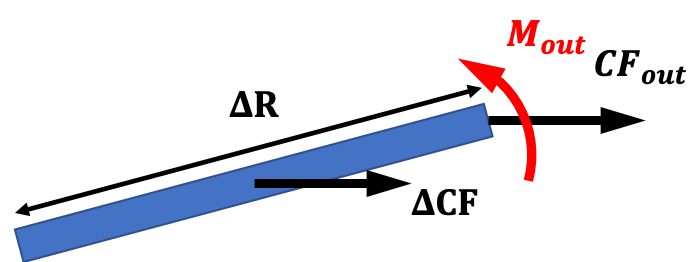
\includegraphics[width=0.75\textwidth]{images/blade_segment.png}
\vspace{-0.1cm}
\caption{Blade spanwise segment}
\label{fig:blade_segment}
\end{center}
\end{figure}

The dominant loads on the outboard end of the segment, that are carried by the spar caps, are the centrifugal force (from all segments outboard of the present one) and a flap bending moment due to (i) distributed lift on segments outboard of the present one, and (ii) a combination of pre-cone and centrifugal load on segments outboard of the present one. The blade spanwise segments are successively sized starting from the tip segment and ending in the root segment. A schematic of the rotor blade segment and cross-section is shown in Fig.~\ref{fig:blade_sizing}.

\begin{figure}
         \centering
		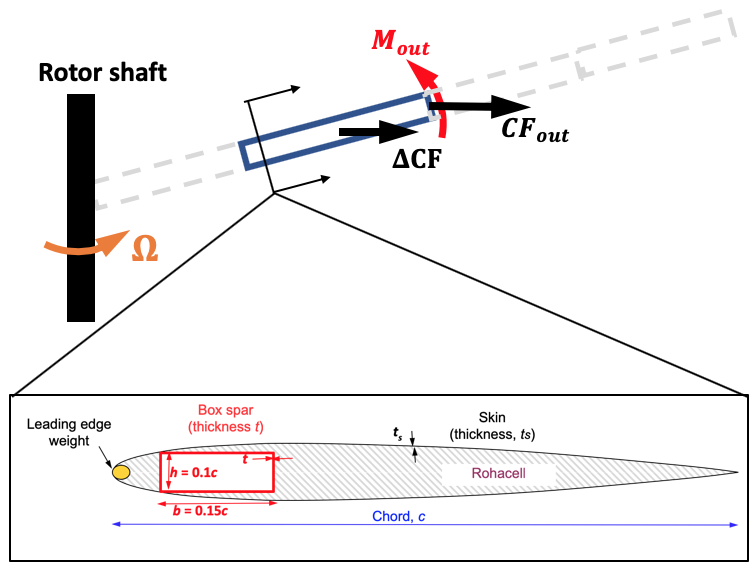
\includegraphics[width=0.7\textwidth]{images/rotor_sizing.png}
        \caption{Rotor blade segment sizing: schematic}
        \label{fig:blade_sizing}
\end{figure}

The total centrifugal load and flap bending moment at the inboard end of the segment is 
\begin{align}
\label{eqns:cfbma}
CF(x_{\rm in}) \quad &= \quad CF(x_{\rm out}) \pls \Delta CF \\
\label{eqns:cfbmb}
M(x_{\rm in}) \quad &= \quad M(x_{\rm out}) \pls \Delta M 
\end{align}
The flap bending moment distribution due to lift, along the non-dimensional span coordinate $x$ (0 at root, 1 at tip) is 
\begin{equation}
M_{\rm lift}(x) \quad = \quad \frac{1}{4} F_z R (x^4 - 4 x + 3)
\end{equation}
The additional centrifugal load and flap bending moment due to loads on the present segment are 
\begin{align*}
\Delta CF \quad &= \quad \frac{1}{2} (m_{\rm s} \pls m_{\rm ns}) V_{\rm TIP}^2 \spc (x){\rm out}^2 \spc - \spc x_{\rm in}^2) \\
\Delta M \quad &= \quad - (CF_{\rm out} + \frac{1}{2} \Delta CF) \Delta R \beta_p \pls M_{\rm lift}(x_{\rm in}) \spc - \spc M_{\rm lift}(x_{\rm out}) 
\end{align*}
The spar mass per unit span is $m_{\rm s})$ and the non-structural mass per unit span is $m_{\rm ns}$.  The maximum axial stress in the spar caps at the inboard end of the present segment is
\begin{equation*}
\sigma_{\rm xx}(x_{\rm in}) \quad = \quad \frac{CF}{A_{spar}} \pls \frac{M(x_{\rm in}) \left(\frac{h}{2}\right)}{2 b t \left(\frac{h}{2}\right)^2}
\end{equation*}

The term $A_{\rm spar}$ is the area of the spar, given by $2 (b+h) t$. The individual expressions can be rearranged to solve for the spar cap thickness $t$, as 
\begin{align*}
t \quad =& \quad \frac{RHS}{LHS} \\
LHS \quad =& \quad \frac{1}{n} \sigma_{\rm max} \pls \frac{1}{2} V_{\rm TIP}^2 (x_{\rm out}^2 - x_{\rm in}^2) \rho_{\rm spar} \spc \left[\Delta R \beta_p \frac{b+h}{bh} - 1 \right] \\
RHS \quad =& \quad \frac{1}{2(b+h)} \left[CF(x_{\rm out}) + \frac{1}{2} m_{\rm ns} V_{\rm TIP}^2 (x_{\rm out}^2 - x_{\rm in}^2) \right] + M_{\rm lift}(x_{\rm in}) \\
& \quad + \spc \frac{1}{bh} \left[ M(x_{\rm out}) \spc-\spc \Delta R \beta_p  \left(CF(x_{\rm out}) \pls \frac{1}{2} \Delta CF\right)\right]
\end{align*}

This formulation avoids iterative convergence inner loops for the rotor blade structure during sizing, improving computational efficiency. 

After sizing the spar, the shear webs thickness is determined from the vertical bending load at the inboard end, given by 
\begin{equation*}
t_{\rm web} \quad = \quad \max\left(\frac{1.5 n V_z}{h \sigma_{\rm skin}},t_{\rm web}\right)
\end{equation*}
Here, $V_z$ is the vertical shear due to blade lift integrated from the inboard end of the segment ($x$=$x_{\rm in}$) to the blade tip ($x$=1). After sizing one spanwise segment, the total axial load and flap bending moment at the inboard end of the segment are calculated using Eqns.~\ref{eqns:cfbma},\ref{eqns:cfbmb} respectively. The loads at the inboard end of the present segment are then assigned as tip loads for the next segment, and the process is repeated for all segments in succession. 

\subsubsection{Root fitting sizing}

The root fitting for the blade is assumed to extend from the shaft ($x$=0) to 10\% of the blade span ($x$=0.1), and is made of 7075 Aluminum. The density is 2800 kg/cu.m, and a limiting axial stress of 20 MPa is used based on a fatigue life of 10$^8$ cycles. The construction of the root fitting is shown in Fig.~\ref{fig:root_fitting}.
 
The tube radius is assumed to be equal to 4$\times$ the airfoil thickness, and the thickness $t_{\rm Root}$ is evaluated to ensure that the maximum tensile stress in the material does not exceed the limiting stress (20 MPa). The tube thickness is solved analytically, using a formulation similar to the approach used for spar sizing. The expression for tube thickness is 
\begin{align*}
t_{\rm Root} \quad = & \quad \frac{RHS}{LHS} \\
RHS \quad = & \quad \frac{CF(x=0.1)}{2 \pi r_{\rm Root} \sigma_{\rm limit}} \pls \frac{M_{\rm lift}(x=0.1)-M_{\rm CF}(x=0.1)}{3 \pi r_{\rm Root}^2 \sigma_{\rm limit}} \\
LHS \quad = & \quad 1 \spc-\spc \frac{\rho}{2 \sigma_{\rm limit}} \Omega^2 (0.1 R) 
\end{align*}
The root fitting thickness is set to the larger of minimum gauge $t_{\rm min}$ or the calculated thickness above, whichever is larger. 

\begin{figure}
\begin{center}
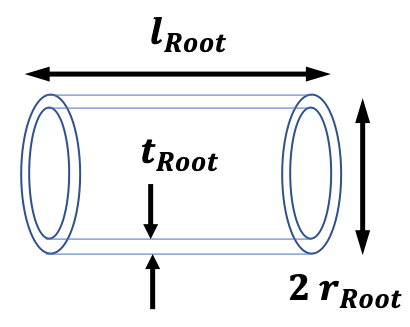
\includegraphics[width=0.4\textwidth]{images/root_fitting.png}
\vspace{-0.1cm}
\caption{Blade root fitting}
\label{fig:root_fitting}
\end{center}
\end{figure}

\subsubsection{Torsion frequency check}
The skin thickness is used to calculate the first elastic torsion frequency for the rotating blade and ensure that it is above 3.3/rev at the hover RPM. If the torsion frequency is too low, then additional skin thickness is added until this requirement is satisfied, preserving the same spar design.

\subsection{Flight controls}
\noindent Two categories of actuators are modeled: fixed-wing, and rotary-wing. 
\subsubsection{Rotor controls}
Unlike large rotorcraft, some eVTOLs feature low-bandwidth collective actuators and no cyclic or swashplate. In such designs, the collective pitch (e.g., for prop-rotors) is usually scheduled with airspeed, and RPM is used for feedback control. Sizing laws for these collective actuators are therefore markedly different from those used for full-scale helicopter controls. The rotor hub mass and collective pitch actuator masses scale with tip speed $V_{\rm TIP}$ (and blade chord $c$ for the actuator) as 
\begin{align}
M_{\rm hub} \spc ({\rm kg})\quad &= \quad 4.84 \left(\frac{V_{\rm TIP}}{171}\right)^2 \left(\frac{c}{0.82}\right) \\
M_{\rm act} \spc ({\rm kg})\quad &= \quad 1.47 \left(\frac{V_{\rm TIP}}{171}\right)^2 \left(\frac{c}{0.82}\right)
\end{align}
The tip speed $V_{\rm TIP}$ is in m/s and mean blade chord $c$ is in meters. 
\subsubsection{Fixed wing controls}
Fixed wing flap and actuator weights are obtained from the AFDD model as 
\begin{equation}
W_{\rm flaps} \spc (lb) \quad = \quad 0.01735 W^{0.644} S_{\rm wing}^{0.41}
\end{equation}
For this model, the weights are in lbs, including the take-off weight $W$. The term $S_{\rm wing}$ is the total plan-form area of all fixed wings, and the actuator weights $W_{\rm flaps}$ includes all actuators on all fixed wings.

\subsubsection{Tilt actuators}
For tilt-rotors and tilt-wing configurations, the masses of tilt actuators are estimated as the larger of 15.5\% of wing mass, and 3.61\% of the total mass being tilted by that actuator. For tilt-wings, both metrics are applicable; for tilt-rotors, the tilt actuator weight is set to 10\% of the masses being tilted.
\begin{align}
M_{\rm tilt-wing} \quad &= \quad \max(0.155 M_{\rm wing}, 0.0361 M_{\rm tilt}) \\
M_{\rm tilt-rotor} \quad &= \quad 0.10 (M_{\rm hub} + M_{\rm act} + M_{\rm blades} + M_{\rm motor}) 
\end{align}

\subsection{Motor mount mass}
\begin{figure} 
\begin{center}
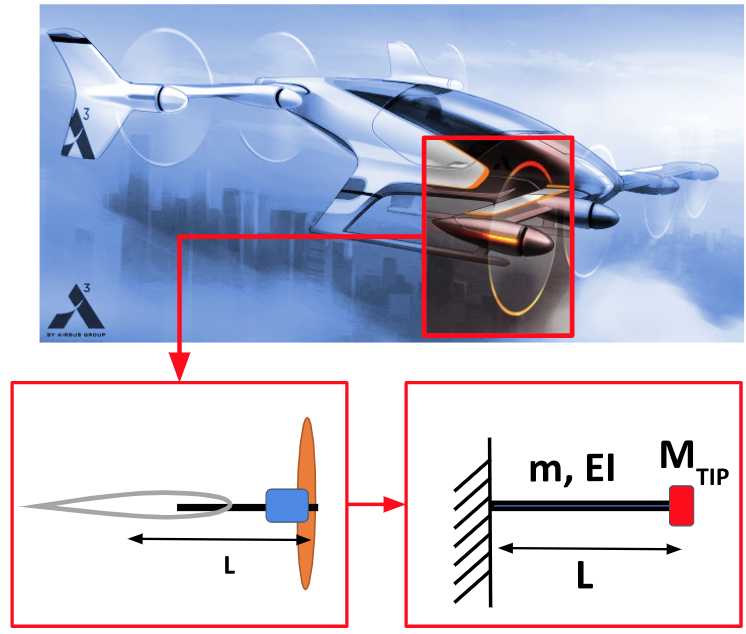
\includegraphics[width=0.6\textwidth]{images/motor_mount.png}
\caption{Motor mount model}
\label{fig:motor_mount}
\end{center}
\end{figure}

The motor mount structure refers to the overhang beam connecting the motor and rotor hub, to a wing (or fuselage). For the Vahana tilt-wing configuration, the motor mount structure is the overhang beam used to offset the rotor hub ahead of the wing leading edge, as shown in Fig.~\ref{fig:motor_mount}. The motor mount is modeled as a cantilever beam of length \textbf{L} with a tip mass equal to the mass of the rotor hub, blades and motor. This structure is sized by a natural frequency requirement, i.e., \textbf{the first cantilever bending mode for this beam with a tip mass} must be sufficiently large so that the structural dynamics do not interact with flight dynamics (0 - 4 Hz). For eVTOLs, a target first bending frequency of 8.5 -- 10 Hz is used to size the motor mount beam. The overhang length is set to the sum of wing three-quarter chord and one rotor radius.

For configurations such as CityAirbus (quad-ducted-coaxial rotors) with no fixed wings, the rotors are mounted directly on the fuselage using support arms. The support arms are treated as ``motor mounts'', and the beam length is set to 120\% rotor radius. Appendix A provides an analytical solution for sizing a cantilever beam with several lumped non-structural masses, distributed structural and non-structural masses based on a target frequency. 

\subsection{Wing weight model}
Three models are available to estimate the weight of a fixed wing:

\subsubsection{AFDD wing weight model}
The weight of a fixed wing is estimated as 
\begin{equation*}
W_{\rm wing} \quad = \quad 5.6641 \frac{\left(\frac{L_w}{1000}\right)^{0.847} n_z^{0.4} S_{\rm wing}^{0.21} AR^{0.5}}{\left(\frac{t}{c}\right)^{0.0936}}
\end{equation*}
The wing weight is in lbs, $L_w$ is the wing design lift in lbs, $n_z$ is the design ultimate load factor, $S_{\rm wing}$ is the wing plan-form area in sq. ft, $AR$ is the wing aspect ratio and $\left(\frac{t}{c}\right)$ is the wing thickness to chord ratio. 

\subsubsection{Frequency tuning: bending loads}
The wing spar is idealized as a cantilever beam with lumped non-structural masses (rotor blades, hub and collective actuator assembly and motor), distributed non-structural masses (skin, ribs) and a hollow circular spar. A schematic of one half-wing is shown in Fig.~\ref{fig:wing_layout}. 

\begin{figure} 
\begin{center}
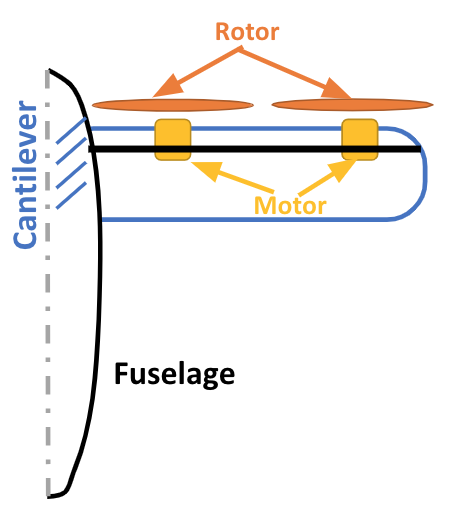
\includegraphics[width=0.35\textwidth]{images/wing_layout.png}
\caption{Wing structure: layout}
\label{fig:wing_layout}
\end{center}
\end{figure}

The wing taper ratio $\lambda$ = $\frac{c_{\rm TIP}}{c_{\rm ROOT}}$ is a design parameter with a default value of 0.75. A tapered wing shifts the non-structural skin mass inboard while strengthening the root, resulting in increased first bending frequency for the same mass. The skin thickness is set to include three layers of carbn fiber (45/0/45), resulting in an areal mass density of $\approx$ 4.9 kg/sq.m. During sizing, the rotor assembly mass and motor mass are used to calculate the wing spar thickness required to achieve a target first bending frequency using the Rayleigh-Ritz approximation detailed in Appendix A. To decouple wing structural dynamics from vehicle flight dynamics, a target first bending frequency of at least 4 Hz is desirable (for a take off mass of 2000 kg). Larger aircraft feature progressively relaxed natural frequency constraints, because the flight dynamic frequencies are lower for larger vehicles with correspondingly larger moments inertia.

\subsubsection{Hover: shear loads}
After determining the spar thickness based on natural frequency requirements, the wing structure is analyzed with static loads in hover with the tapered beam. Rotor thrusts are applied at the motor mount locations and the static bending stresses and shear stresses are calculated at five points between nodes (nodes are located at the root and motor mount locations). A load factor of 3.8 and safety margin of 1.5 are applied to ensure that the spar can support the loads in hover. This hover loading condition is more limiting than cruise flight with the same load factors and safety factors, because the bending moments due to distributed lift are lower than the corresponding bending moments in hover. The shear loading is used to estimate the number of $\pm$ 45 deg layers of carbon fiber, while the bending loads are supported by layers of uniaxial carbon fiber. 

\subsection{Airframe Weight Model}
\subsubsection{Statistical weight model}
The AFDD82 fuselage weight model for helicopter is given by
\begin{equation}
w_{\rm fuselage} = w_{\rm basic} + w_{\rm press} + w_{\rm cw}
\end{equation}
where $w_{basic}$ is the basic weight of the fuselage, $w_{\rm press}$ is the weight from any pressurization constraints (set to none for the sample mission in this work) and $w_{\rm cw}$ is the weight addition for crashworthiness, which is assumed to be 6\% of the basic weight as per AFDD standards. The basic weight is given by
\begin{equation}
\label{eqn:afdd82_fuselage}
w_{\rm basic} = 5.896 f_{\rm ramp} \left(\frac{W_{\rm GTOW}}{1000} \right) ^ {0.4908} n_z ^ {0.1323} S_{\rm body}^{0.2544} l^{0.61}
\end{equation}
where $f_{\rm ramp}$ is the factor for a retractable ramp, $n_z$ is the load factor, $S_{\rm body}$ is the wetted area of the fuselage (sq. ft) and $l$ is the length of the fuselage (feet). While these terms can be defined for full-scale helicopters/tiltrotor, their definitions become increasingly challenging to interpret in the context of unconventional configurations such as an eVTOL, with very different load paths compared to helicopters. %Additionally, even if such a definition can be codified, the error in the model at small take-off weights (less than one ton) is significant (up to 10\% or more). 
\subsubsection{Physics-based weight model}
A physics-based model is used to estimate the weights of load-bearing components that transmit rotor hub forces and wing lift and drag to the vehicle center of mass. The airframe is subdivided into 3-D beam elements, each with bending, axial and torsion degrees of freedom. Rotor hub loads and wing lift/drag are modeled as point loads at the motor points, and distributed uniformly over the wing span, respectively. The external loads corresponding to each mission phase are applied on the structure,  (rotor thrust, torque, wing lift and wing drag) and the resulting stresses and deflections are calculated and stored at all the nodes. Subsequently, the cross-section dimensions of the beams are iteratively resized to ensure; (i) Minimum factor of safety of 1.5 (based on Von-Mises stress) at a load factor of 3.5, (ii) A maximum deflection of 10\% for any node (relative to its distance from the vehicle center). The cross-sections of all beam elements are assumed to be hollow circles with wall thickness equal to 15\% outer radius. The only design parameter for a beam element is the outer radius of the cross-section. Beam cross-section radii for all elements are updated iteratively until the 3 design criteria are satisfied, and the weight of the airframe members is calculated using material density and final dimensions. The finite element analysis iterations are performed within the sizing loop. The parameterization for a quad-rotor layout is shown in Fig.~\ref{fig:airframe}.

\begin{figure}
\begin{center}
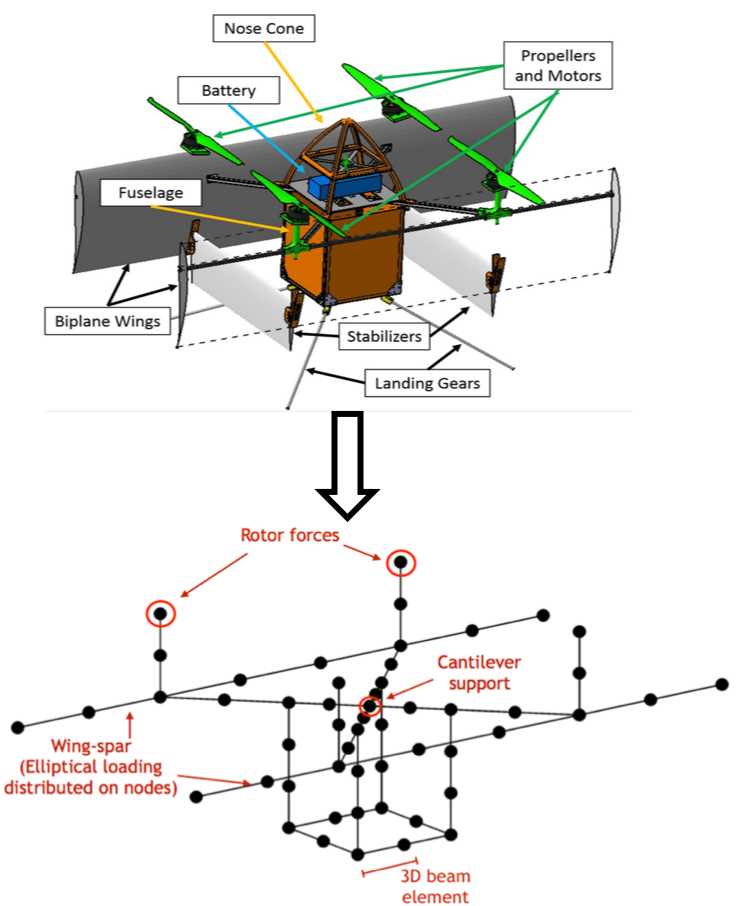
\includegraphics[width=0.65\textwidth]{images/airframe.png}
\vspace{-0.1cm}
\caption{Quad-rotor biplane tail-sitter: layout to finite element representation}
\label{fig:airframe}
\end{center}
\end{figure}

\begin{figure}
\begin{center}
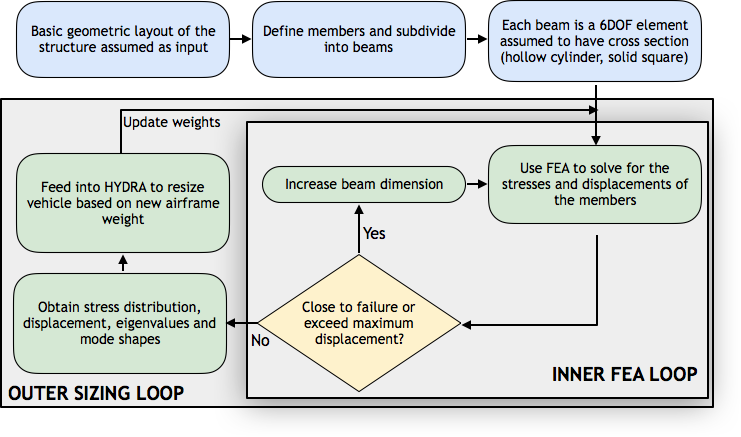
\includegraphics[width=0.75\textwidth]{images/fea_flowchart.png}
\vspace{-0.1cm}
\caption{Workflow for including physics-based airframe weight model in sizing}
\label{fig:fea_flowchart}
\end{center}
\end{figure}

\noindent \textbf{Integration of FEA into sizing: workflow} \\
%In the present work, the airframe is defined as a beam lattice framework and the loads on the structure are computed using a finite element analysis (FEA). The external loads on the structure arise from the weight of different components and the dominant aerodynamics loads (rotor thrust and wing lift). A set of three-dimensional Euler-Bernoulli beam elements with six degrees of freedom at each node (three translations and three rotations) was assembled in a finite element framework. After discretization of the distributed loads into equivalent concentrated forces and moments at wing nodes, the static deflection is obtained and used to compute bending stresses. By requiring each element in the structure to operate within a band of a target safety factor, and not exceed a maximum absolute limit for bending deflection, beam cross-section dimensions are iteratively adjusted in an inner loop within the sizing framework. 
\noindent The overall process is depicted in a flowchart shown in Fig.~\ref{fig:fea_flowchart} and proceeds as follows
\begin{enumerate}
\item {\bf Initialize: } A geometric layout of the airframe is chosen, and beam elements are defined. The present work assumes the beam cross section to be simple shapes such as a hollow cylinder or a solid square.

\item {\bf Inner FEA loop: } Point forces and moments are applied to the structure based on rotor and wing loads, such as rotor thrust, rotor torque and wing lift. The von-Mises stress ($\sigma_{\rm VM}$), the corresponding factor of safety and deflection of the various nodes are computed as
\begin{eqnarray}
\sigma_{\rm VM} &=& [ (\sigma_{xx}-\sigma_{yy})^2 + (\sigma_{yy}-\sigma_{zz})^2   \\ \nonumber
&+& (\sigma_{zz}-\sigma_{xx})^2 + 6(\sigma_{yz}^2+\sigma_{xy}^2+\sigma_{xz}^2) ]^{1/2}
\end{eqnarray}
where $\sigma_{\rm ij}$ are components of the stress tensor and the factor-of-safety (FOS) is
\begin{equation}
{\rm FOS} = {\rm min}(\sigma_{VM})_i / \sigma_{\rm yield} \qquad  \ \forall\ \ i\ \in N
\end{equation}
where $N$ is the total number of beam elements.

\item {\bf Update cross-section dimensions: } The mathematical constraints imposed for convergence are
\begin{equation}
|{\rm FOS}_{\rm tar} - \Delta {\rm FOS}| \leq {\rm min}({\rm FOS})
\end{equation}
% \leq {\rm FOS}_{\rm tar} + \Delta {\rm FOS}
where ${\rm FOS}_{\rm tar}$ is the target FOS, set to 1.5 and $\Delta {\rm FOS}$ is the allowable band, set to 0.1. The axial and bending deflections of each node are normalized by the distance of the node from the vehicle center of gravity. These normalized deflections must not exceed a pre-determined fraction (0.08) to ensure structural rigidity. Depending on the type of condition encountered, two types of cross-section updates are calculated:
\begin{enumerate}
\item The beam cross-section is scaled up by the term (FOS/FOS$_{\rm tar}$)$^{1/3}$) if the factor of safety is not sufficiently large. The cube root in the expression stems from the fact that stress is inversely proportional to cross-section dimension under static load.
\item If the deflection of any one node is too large, the dimensions of all cross-sections are increased by 10\%. Increasing the sizes of all the member cross-sections is required because adding stiffness to the root end of a longer beam may be more effective than stiffening an outboard member (in the present workflow, no apriori assumptions are made about the load path, and so to guarantee deflections are restricted, all members are stiffened).
\end{enumerate}
The larger of the two calculated dimensions for each structural member is provided to the FEA for the next iteration. The stresses and deflections are recalculated, and members resized until the structure achieves the required factor of safety and deflection limits.

The airframe weight is computed by multiplying the total volume of all the beam elements with the material density (Aluminum, 2,700 kg/m$^3$ or carbon, 1650 kg/m$^3$). This converged airframe weight from static finite element analysis replaces the fuselage weight from the AFDD empty weight formulae in the iterative sizing process.

\end{enumerate}
The structural analysis used in in sizing the airframe structure also provides estimates of the natural frequencies and the mode-shapes. This information can be used in advanced stages of design to ensure sufficient separation between the airframe, blade natural frequencies and operating RPM range of the rotor(s). 

\subsection{Weight margin}
A weight margin is included in the analysis to admit additional expansion of component performance (and therefore weight) at later stages of design. Therefore, \textbf{10\% of the vehicle empty weight} is allocated for a weight margin. 

\subsection{Fixed weight groups}
Fixed empty weight groups consist of mission-specific components and do not scale with vehicle dimensions or system performance during sizing. These fixed weight groups are 
\begin{enumerate}
\item Carpets, cabin trim and noise insulation
\item Avionics, sensors and flight computers
\item Airconditioning and heaters
\item Seats
\item Low voltage battery, anti-collision lights, air data systems 
\item High voltage bus and power distributors
\end{enumerate} 			% Theory manual
%\section{\textbf{Analysis Organization}}

\hydra \spc is a rotorcraft sizing code with the following features:
\begin{enumerate}
\item \textbf{Sizing}: obtain consistent vehicle weights and performance for a given payload and mission profile.
\item \textbf{Optimization} Optimize a given design (e.g., for annual operating cost) 
\item \textbf{Sensitivity Analysis} For a given design, identify sensitivity of weights and performance metrics to (i) underlying assumptions (e.g., engine efficiency), and (ii) changing design variables (e.g., rotor tip speed)
\end{enumerate}

The main focus of this document is to explain the usage of the analysis, and implementation of the various performance, weight and cost models used to size the rotorcraft. The theory, if any, will be explained side-by-side with the corresponding code segment. 

\subsection{\textbf{Programming Language and Syntax}}
\hydra \spc is written in \ty{Python3}, with heavy emphasis on classes to contain and compartmentalize information. Because \ty{Python2} support expires in 2019, it is recommended to use \ty{Python3} specifically.

Some parts of the code are written in \ty{Fortran}. Three fortran compilers have been tested and verified to work with the compiled parts of the code: GNU fortran, intel fortran and PGI fortran. Among these three compilers, \ty{gfortran} and \ty{pgfortran} are free, while \ty{ifort} requires academic or commercial licenses. The main advantage of \ty{pgfortran} is the availability of support for \ty{CUDA-Fortran}, while executables generated with \ty{ifort} consistently run faster than those generated with \ty{gfortran} or \ty{pgfortran} for the target applications. 

\hydra \spc also features a built-in Blade Element Momentum Theory (BEMT) solver, also implemented in \ty{Fortran90}. The BEMT solver is parallelized with \ty{OpenMP}. Additionally, the sizing and optimization stages of \hydra \spc are parallelized with \ty{MPI}, and can be executed in parallel.

\subsection{\textbf{Pre-Requisites and Installation Notes}}
A \textbf{Fortran90 compiler} is required. Due to the use of free-format coding, derived types and modules, \emph{a Fortran77 compiler is not sufficient}. 

If you want to try running the code on Windows, there are some manual steps required to help certain Python modules recognize the OpenMP libraries. For the time being, consult Ananth for installation details on Windows. 

Additional \textbf{Python3} and its modules (freely available) are required to run HYDRA and its various postprocessors:
\begin{enumerate}
	\item \textbf{matplotlib, numpy, scipy, pyyaml, python3-tk, f90wrap}
	\item Optional: mpi4py
\end{enumerate}

Finally, \textbf{CMake} version 3.0 or higher is required to create Platform-independent Makefiles that compile the Fortran90 routines. To use integrated \LaTeX rendering for fonts in plots, you may also need the \textbf{texlive-fonts-extra} package.

\subsection{\textbf{Source Code Directories}}
All source code to be compiled is located in \textbf{src/}, under various subfolders. Each subfolder contains a collection of subroutines or functions that pertain to specific types of operations. 

\subsubsection{\textbf{Python code: src/Python}}
This subfolder contains various classes and functions written in Python that pertain to sizing a vehicle, in four sub-folders.
\begin{enumerate}
      \item \textbf{Stage\_0/}: This folder contains the ``main'' class that defines the vehicle in \textbf{hydraInterface.py}. It contains the various high-level driver functions pertaining to sizing and optimization. The folder also contains two other files, \textbf{dict2obj.py} (convert dictionary to class) and \textbf{footprint.py} (calculates vehicle footprint).
      \item \textbf{Stage\_1/}: This folder contains the workhorse routines that perform sizing with weight, performance and cost estimation.
      \item \textbf{Stage\_3/}: This folder contains Python-wrapped routines for higher-fidelity fuselage and wing weight models, BEMT rotor performance models and the associated interfaces to setup the inputs and extract outputs for the sizing analysis.  
      \item \textbf{Postprocessing/}: This folder contains functions that perform postprocessing analysis, including optimization, design perturbation and sensitivity studies, noise estimation, battery status, profile, power curve, and pie charts for the breakdown of vehicle weight, operating cost and parasitic drag. 
\end{enumerate}

\subsubsection{\textbf{NETLIB FILES: Source/fea/Source/mathops/}}
 This subfolder contains the ODE Solver \ty{dassl}, algebraic equation solver \ty{hybrd} and various dependencies needed for linear algebra and matrix operations. These files have not be modified, except the algebraic equation solver \ty{hybrd.f}. This file alone has been changed to obtain the Jacobian in parallel using OpenMP.
 
Parts of the sizing analyis, FEA-based fuselage/wing weight estimation and BEMT-based rotor performance estimation are written in Fortran90 to improve execution speed. The source code for these operations are contained in \textbf{src/bemt/Source/}, \textbf{src/fea/Source/} and \textbf{src/sizing/Source/}. Within each of these folders, there are three sub-folders: 

\subsubsection{\textbf{Python-integrated routines: Source/pyint\_files/}}
This subfolder contains routines that can be invoked from Python, using \ty{f2py} and James Kermode's \ty{f90wrap} adaptation for derived types.

\subsubsection{\textbf{Python-accesible modules: Source/pyint\_modules/}}
The files in this folder contain module definitions used to define universal constants (e.g., 1, 0, $\pi$) to the required precision. Using James Kermode's \ty{f2py-f90wrap} interface generator, \python \spc can access and modify these module variables directly without having to painstakingly break down derived types into its primitive constituents (arrays, integers, real numbers and logicals). The advantage of this automation and abstraction helps avoid programming errors, reduces the number of arguments passed between \ty{Python} and \ty{Fortran} and allows for code feature expansion without significant additional effort.

\subsubsection{\textbf{Python-invisible files: Source/pyinv\_files/}}
The files in this folder are work-horse routines that can be called only by the routines in \textbf{Source/pyint\_files/}, but not directly by \python. These routines, together with those in Source/pyint\_files/, are compiled into shared object files. Specific routines (present in Source/pyint\_files/) in these shared objects can be called by the \python \spc interface.              % code organization
%\section{First-time setup}
\subsection{Installing pre-requisites}
For Debian-based Linux distributions, you can get \ty{Python3}, CMake and gfortran using the command 
\begin{center}
\textbf{sudo apt-get install python3 cmake gfortran texlive-fonts-extra}
\end{center}

For MacOS, similar commands can be executed with brew. 

After installing \ty{Python3}, install various modules using \ty{pip}

\begin{center}
\textbf{sudo python3 -m pip install numpy} \\
\textbf{sudo python3 -m pip install scipy} 
\end{center}

In a similar manner, install the other modules with a terminal.


\subsection{Compiling source code}
After installing the pre-requisites, create the directory \textbf{cmake/build/} as follows

\begin{center}
\textbf{cd cmake/} \\
\textbf{mkdir build/}\\
\textbf{cd build/} 
\end{center}

Then, execute the cmake command and compile the code
\begin{center}
\textbf{FC=gfortran cmake ../../} \\
\textbf{make -j} 
\end{center}

\subsection{MacOS-specific issues}

Hopefully, there are no issues and the build process executes successfully. However, if it does not, and you are reading this, chances are that you are using Windows, or Mac. For Windows, there is a long and complicated series of steps documented here:
\texttt{https://github.com/jameskermode/f90wrap/issues/73}

For MacOS, the system may not recognize the \ty{f90wrap}  and \ty{f2py-f90wrap} commands even if the \textbf{f90wrap} module is installed - this issue was noticed for OSX High Sierra and v3.7 of \python. In case this situation arises, you may have to create symbolic links to these two commands in \ty{/usr/local/bin/}. For example, Ananth had to create a symlink as follows:

\begin{enumerate}
\item Identify where \textbf{f90wrap} is installed: use the following command in terminal
\begin{center}
\textbf{python3 -m site}\\
\end{center}
If \ty{Python3} is installed correctly, you will see an output that looks like this: \\
\begin{lstlisting}
sys.path = [
    '/usr/local/bin',
    '/usr/local/Cellar/python/3.7.0/Frameworks/Python.framework/Versions/3.7/lib/python37.zip',
    '/usr/local/Cellar/python/3.7.0/Frameworks/Python.framework/Versions/3.7/lib/python3.7',
    '/usr/local/Cellar/python/3.7.0/Frameworks/Python.framework/Versions/3.7/lib/python3.7/lib-dynload',
    '/usr/local/lib/python3.7/site-packages',
    '/usr/local/lib/python3.7/site-packages/RBF-2018.10.31-py3.7-macosx-10.13-x86_64.egg',
    '/usr/local/Cellar/python/3.7.0/Frameworks/Python.framework/Versions/3.7/lib/python3.7/site-packages',
    '/usr/local/Cellar/python/3.7.0/Frameworks/Python.framework/Versions/3.7/lib/python3.7/site-packages/RBF-2018.10.31-py3.7-macosx-10.13-x86_64.egg',
]
USER_BASE: '/Users/ananthsridharan/Library/Python/3.7' (doesn't exist)
USER_SITE: '/Users/ananthsridharan/Library/Python/3.7/lib/python/site-packages' (doesn't exist)
ENABLE_USER_SITE: True
\end{lstlisting}

The results of this command show that \textbf{f90wrap} may be found in
\begin{lstlisting}
/usr/local/Cellar/python/3.7.0/Frameworks/Python.framework/Versions/3.7/bin/
\end{lstlisting}

To verify that the \textbf{f90wrap} and \textbf{f2py-f90wrap} commands can indeed be located in that folder, use the \textbf{ls} command as follows: (without the linebreak)
\begin{center}
\textbf{ls /usr/local/Cellar/python/3.7.0/Frameworks/\\
Python.framework/Versions/3.7/bin/*f90wrap}
\end{center}
You should see an output that looks like this:
\begin{lstlisting}
/usr/local/Cellar/python/3.7.0/Frameworks/Python.framework/Versions/3.7/bin/f2py-f90wrap
/usr/local/Cellar/python/3.7.0/Frameworks/Python.framework/Versions/3.7/bin/f90wrap
\end{lstlisting}

Now, we're ready to use the \textbf{ln} command to create symlinks. 

\item First, create a link for f90wrap:

\begin{center}
\textbf{ln -s /usr/local/Cellar/python/3.7.0/Frameworks/ \\
Python.framework/Versions/3.7/bin/f90wrap /usr/local/bin} \\
\end{center}

\item Next, create a link for f2py-f90wrap:

\begin{center}
\textbf{ln -s /usr/local/Cellar/python/3.7.0/Frameworks/ \\
Python.framework/Versions/3.7/bin/f2py-f90wrap /usr/local/bin} \\
\end{center}

\end{enumerate}

Then, try deleting the build directory and redo all the compilation steps.  						% initial setup for the code
%\section{Input files}
This section of the documentation details the inputs files and conventions that that are necessary to perform sizing. \hydra \spc inputs and outputs are handled using \textbf{yaml} files through the \textbf{pyyaml} package. The yaml input files are converted to \python \spc dictionaries when read, allowing the inputs to be specified in any order. The main dictionaries in \textbf{input.yaml} are \textcolor{red}{\textbf{Sizing}}, \textcolor{red}{\textbf{Configuration}}, \textcolor{red}{\textbf{Mission}} and \textcolor{red}{\textbf{Aircraft}}. All four dictionaries must be present in \textbf{input.yaml}. Two example files are shown below with the \textcolor{red}{\textbf{main dictionary names}} and \blue{sub-dictionary names} highlighted. The two main input files are \textbf{input.yaml} and \textbf{defaults.yaml}.

\subsection{Single main rotor helicopter}
\subsection*{Input file 1: input.yaml}
This input file specifies the mission profile, vehicle configuration, propulsion type and masses of fixed weight groups (e.g., crew, payload, mission equipment). The input file is subdivided into multiple segments, and each input and its units are explained in the following sections. The following input file is used to size a single main rotor/tail rotor helicopter with a mechanical transmission and turboshaft engines. An example single main rotor helicopter is shown in Fig.~\ref{fig:helo}.

\begin{figure}[H]
\begin{center}
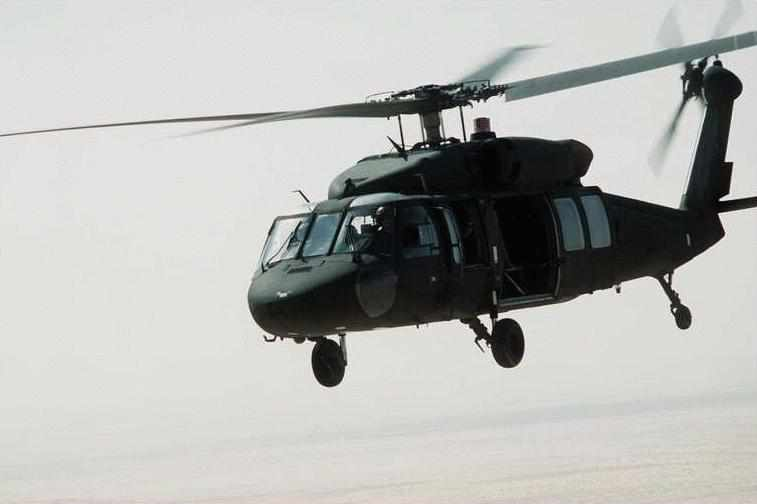
\includegraphics[width=0.5\textwidth]{images/uh60_blackhawk.png}
\caption{UH-60 Blackhawk: single main rotor helicopter}
\label{fig:helo}
\end{center}
\end{figure}

\subsubsection{\red{Sizing} dictionary}
\begin{lstlisting}
<@\textcolor{red}{\textbf{Sizing:}}@>
   <@\blue{Rotors:}@>
      SMR:
         DL:         [10.03]         # lb/ft2
#       radius:     [6.607]          # radius in meters
         Nb:         [4]  
         Vtip:       [213.36] # m/s
         solidity:   [0.1178]
         tip_mach:   [0.95]
         flap_freq:  [1.035]
         cruise_rpm_ratio:  [1.0]
   <@\blue{Fuselage:}@>
      nrotors:         [1]
      liftfraction:    [1.0]
   <@\blue{Powerplant:}@>
      TSEngine: 
         type: `turboshaft'
         num:  2
         redundancy: 0        # how many units can fail, group still works
   <@\blue{Transmission:}@>
      Trans1: 
         type:       `mechanical'
         eta:        0.98
#fidelity options for weight and performance models
   ifea:               False
   use_bemt:           False
\end{lstlisting}

The \red{Sizing} dictionary specifies the values of high-level design variables to use for vehicle sizing. Up to five sub-dictionaries (\blue{Rotor}, \blue{Wings}, \blue{Fuselage}, \blue{Transmission}, and \blue{Powerplant}) and two logical inputs for using higher-fidelity models constitute the sizing dictionary.
\paragraph{\blue{Rotors}}
\blue{Rotors} consists of sub-dictionaries, with each sub-dictionary corresponding to a rotor. In the present example, there is only one rotor that is sized by user-given inputs. The rotor that is sized is the main rotor, called ``SMR'' (Single Main Rotor). The actual name of the rotor can be any string, i.e., \texttt{SMR} is not a keyword, but \texttt{\blue{Rotors}} is a keyword. If neither of these keywords are specified, then the rotor group must be mounted on wings, and its diameter is determined from geometric requirements (largest rotor that fits on all wings that the rotor is mounted on, with adequate rotor-rotor clearance and rotor-fuselage spacing).
\begin{lstlisting}
   <@\blue{Rotors:}@>
      SMR:
         DL:         [10.03]         # lb/ft2
#       radius:     [6.607]          # radius in meters
         Nb:         [4]  
         Vtip:       [213.36] # m/s
         solidity:   [0.1178]
         tip_mach:   [0.95]
         flap_freq:  [1.035]
         cruise_rpm_ratio:  [1.0]
\end{lstlisting}
\noindent ``SMR'' is parameterized using the following \textbf{keywords} shown in Table~\ref{tbl:rotor_keywords}. The last keyword \textcolor{gray}{\textbf{radius}} is grayed out, because it is not used in the present example (the corresponding line in the input file is commented out, indicated by the `\#' symbol). The \textbf{radius} keyword may be specified as an alternate to rotor disk loading. 

\paragraph{\blue{Fuselage}}
The \blue{Fuselage} dictionary is shown below, and the keywords used to define the fuselage are shown in Table~\ref{tbl:fuselage_keywords}.
\begin{lstlisting}
   <@\blue{Fuselage:}@>
      nrotors:         [1]
      liftfraction:    [1.0]
\end{lstlisting}

\begin{center}
  \begin{table}[H]
	\caption{Keywords for sizing a helicopter rotor}
	\label{tbl:rotor_keywords}
    \begin{tabular}{| c | l | c |}
    \hline
    Keyword & Meaning & Value in example \\ 
    \hline
\textbf{DL} & Disk loading & 10.03 lb/ft$^2$ \\
\textbf{Nb} & Number of blades & 4 \\
\textbf{Vtip} & Rotor hover tip speed & 213.36 m/s \\
\textbf{solidity} & Geometric solidity & 0.1178 \\
\textbf{tip\_mach} & Maximum blade tip Mach number & 0.95 \\
\textbf{flap\_freq} & First flap natural frequency in hover & 1.035/rev \\
\textbf{cruise\_rpm\_ratio} & Rotor cruise RPM/hover RPM & 1.0\\
\textcolor{gray}{\textbf{radius}} & \textcolor{gray}{Rotor radius} & \textcolor{gray}{6.607 m} \\
    \hline
  \end{tabular}
\end{table}
\end{center}
%\vspace{-1cm}
\begin{center}
  \begin{table}[H]
	\caption{Keywords for sizing a fuselage}
	\label{tbl:fuselage_keywords}
    \begin{tabular}{| c | l | c |}
    \hline
    Keyword & Meaning & Value in example \\ 
    \hline
\textbf{nrotors} & Number of rotors mounted on this fuselage & 1 \\
\textbf{liftfraction} & Lift fraction carried by fuselage-mounted rotors & 1.0 \\
    \hline
  \end{tabular}
\end{table}
\end{center}

\paragraph{\blue{Powerplant}}
The \blue{Powerplant} definition is shown below. There is only one powerplant group, called `TSEngine' (TurboShaft Engine). 
\begin{lstlisting}
   <@\blue{Powerplant:}@>
      TSEngine: 
         type: `turboshaft'
         num:  2
         redundancy: 0        # how many units can fail, group still works
\end{lstlisting}
Here, `TSEngine' is not a keyword: it is only the name given to the powerplant group, just as `SMR' is the name of the rotor group. This powerplant group is defined using the keywords shown in Table~\ref{tbl:powerplant_keywords}. Here, there are two turboshaft engines, sized so that no engines may fail if adequate power is required in all segments of the sizing mission (excluding margins - specified later in defaults.yaml, Engine parameters ).

\begin{table}[H]
\begin{center}
	\caption{Keywords for sizing a powerplant}
	\label{tbl:powerplant_keywords}
    \begin{tabular}{| c | l | c |}
    \hline
    Keyword & Meaning & Value in example \\ 
    \hline
\textbf{type} & Type of powerplant, character string & `turboshaft' \\
\textbf{num} & Number of engines/units & 2  \\
\textbf{redundancy} & No. of unit failures allowed & 0 \\
    \hline
  \end{tabular}
\end{center}
\end{table}
\vspace{-1.5cm}

\paragraph{\blue{Transmission}}
The \blue{transmission} input block is shown below. There is only one transmission in this conventional helicopter, named `Trans1'. The name of the transmission group (Trans1) is not a keyword, but the attributes of this transmission group are defined using keywords described in Table~\ref{tbl:transmission_keywords}.

\begin{lstlisting}
   <@\blue{Transmission:}@>
      Trans1: 
         type:       `mechanical'
         eta:        0.98
\end{lstlisting}

  \begin{table}[H]
\begin{center}
	\caption{Keywords for sizing a transmission}
	\label{tbl:transmission_keywords}
    \begin{tabular}{| c | l | c |}
    \hline
    Keyword & Meaning & Value in example \\ 
    \hline
\textbf{type} & Type of transmission, character string & `mechanical' \\
\textbf{eta} & Transmission efficiency (power out/power in) & 0.98  \\
    \hline
  \end{tabular}
\end{center}
\end{table}
\vspace{-1.5cm}

\paragraph{High-fidelity model switches}
The keyword \textbf{ifea} is a logical input, used to specify if the FEA-based weight model is to be used in the sizing loop to estimate the airframe structural weight. The other keyword \textbf{use\_bemt} indicates whether the Blade Element Momentum Theory (BEMT) should be used to refine rotor performance estimates in hover (and cruise for prop-rotors). In this example, both options are not enabled. 

\subsubsection{Aircraft \red{Configuration}}
The \red{Configuration} dictionary specifies the associations between rotors, wings (if present), fuselage, transmissions and powerplants (defined in the \red{Sizing} dictionary). This dictionary provides the crucial mapping that specifies where rotors are mounted, and the transmissions connecting various powerplants to the rotor groups. The group names (SMR, Trans1 and TSEngine) are used to specify these connections and size power sources using rotor power required and transmission efficiencies. 

\begin{lstlisting}
<@\red{Configuration:}@>
   <@\blue{Fuselage:}@> `SMR'                 # which rotors are mounted on fuselage
   <@\blue{Rotors:}@>
      SMR: `Trans1'                 # transmission used to power the rotors
   <@\blue{Transmission:}@>                   # powerplant connected to transmissions
      Trans1:                       # transmission group name 
         Powerplant: `TSEngine'     # powerplant group name
         PowerFraction: 1.0         # rated power fraction supplied 
\end{lstlisting}

The various keywords used to associate vehicle components are explained in Table~\ref{tbl:config_smr}. The associations between rotors, fuselages and wings are specified as key-value pairs. The present example is interpreted by \hydra \spc as
\begin{enumerate}
\item The \blue{Fuselage} supports the rotor group called `\texttt{SMR}' 
\item The \blue{Rotors} dictionary specifies that the rotor group \texttt{SMR} draws power through the transmission group `\texttt{Trans1}'
\item The \blue{Transmission} dictionary specifies that the transmission group \texttt{Trans1} draws 100\% of its required power from the powerplant group \texttt{`TSEngine'}.
\end{enumerate}
  \begin{table}[H]
\begin{center}
	\caption{Keywords for defining vehicle configuration}
	\label{tbl:config_smr}
    \begin{tabular}{| c | l | c |}
    \hline
    Keyword & Meaning & Value in example \\ 
    \hline
\textbf{Fuselage} & Specifies rotor mounted on fuselage & `SMR' \\
\textbf{Rotors} & Specifies transmissions powering each rotor group & SMR: `Trans1' \\
\textbf{Transmission} & Sub-dictionaries specify transmission details & `Trans1' \\
\textbf{Powerplant} & Following name specifies associated powerplant & `TSEngine' \\
\textbf{PowerFraction} & Fraction of rated power from `TSEngine' above & 1.0 \\
    \hline
  \end{tabular}
\end{center}
\end{table}
\vspace{-1cm}
\subsubsection{\red{Mission profile}}
The sizing mission profile is specified through several keywords; the meaning of these keywords is explained below, and summarized in Table~\ref{tbl:mission_keywords}. 

The parameter \textbf{nsegments} specifies the number of mission segments. Each segment type can be `hover' or `cruise', specified by the parameter \textbf{flight\_mode}. For hover segments, the duration is specified by the parameter \textbf{time\_seg}. For cruise segments, either the segment duration can be specified, or the \textbf{distance} can be provided as an input and the segment velocity \textbf{cruise\_speed} will be calculated. If the distance is provided as a non-zero input value, the cruise segment duration input is ignored. For climb segments, the start and end altitudes \textbf{start\_altitude}, \textbf{end\_altitude} are specified in meters. 

The parameter \textbf{add\_payload} is used to inform the analysis that the payload has changed at the end of a mission segment (e.g., cargo picked up/dropped off or passenger disembarked/entered the vehicle). The input parameter \textbf{segment\_type} specifies the type of mission segment - `all' indicates the segment is used in day-to-day operations, while `reserve' indicates that the segment is used for sizing, nut not operating cost calculations. The parameter \textbf{sizing\_order} is a list of integers, with zero specifying that the segment is not used for sizing, and a non-zero integer specifying that the segment is used to size a particular component. Usually, the first hover segment and first cruise segment are used for sizing various components. The final line is an optional input specifying the parameter \textbf{fixed\_GTOW}. If this line is present, it instructs the analysis to run sizing in fixed take-off weight mode, and estimate the payload.

\begin{lstlisting}
<@\red{Mission:}@>
   nsegments:          5
   flight_mode:        [ 'hover', 'cruise', 'cruise', 'cruise', 'cruise'] 
   segment_type:       [ 'all',    'all',    'all',    'all',    'all'] 
   time_seg:           [      5,     2.42,     8.23,     84.9,        5] # minutes
   start_altitude:     [ 1219.2,   1219.2,   1828.8,   1828.8,      0.0] # m
   end_altitude:       [ 1219.2,   1828.8,   1828.8,   1828.8,      0.0] # m
   delta_temp_isa:     [ 27.92,    11.88,         0,        0,        0] # deg C
   rate_of_climb:      [      0,   251.86,        0,        0,        0] # m/min
   cruise_speed:       [      0,    85.33,   157.16,   159.03,    70.74] # knots
   add_payload:        [      0,        0,        0,        0,        0] # 
   distance:           [      0,      0.0,    39.93,    416.7,      0.0] # km
   fixed_GTOW:         6454.0               # derive payload for fixed weight
\end{lstlisting}

\begin{center}
  \begin{table}[H]
	\caption{Keywords for defining mission}
	\label{tbl:mission_keywords}
    \begin{tabular}{| c | l | c |}
    \hline
    Keyword & Meaning & Value in example \\ 
    \hline
\textbf{nsegments} & Number of segments in sizing mission & 6 \\
\textbf{flight\_mode} & Specifies type of mission segment & `hover', `cruise' \\
\textbf{time\_seg} & Segment duration in minutes & \textcolor{gray}{--} \\
\textbf{start\_altitude} & Altitude at start of segment (m) & \textcolor{gray}{--} \\
\textbf{end\_altitude} & Altitude at end of segment (m) & \textcolor{gray}{--} \\
\textbf{delta\_temp\_isa} & Temperature offset at sea level (C) & \textcolor{gray}{--} \\
\textbf{rate\_of\_climb} & Vehicle rate of climb in the segment (m/min) & \textcolor{gray}{--} \\
\textbf{cruise\_speed} & Horizontal speed parallel to ground (knots) & \textcolor{gray}{--} \\
\textbf{add\_payload} & Payload added at end of segment (kg) & \textcolor{gray}{--} \\
\textbf{distance} & Horizontal distance covered (km) & \textcolor{gray}{--} \\
\textbf{fixed\_GTOW} & Total weight to hold constant (kg) & \textcolor{gray}{--} \\
     \hline
  \end{tabular}
\end{table}
\end{center}

\subsubsection{\red{Aircraft} details}
The aircraft specification dictionary is show below, and the relevant keywords are summarized in Table~\ref{tbl:aircraft_keywords}. The payload mass, crew mass, common equipment and avionics mass are fixed mass groups, specified in kg. The parameter \textbf{common\_per\_pax} is the mass of equipment that is multiplied by the number of passengers, specified by \textbf{pax\_count}. Based on the number of passengers, additional payload is added internally with the following map: 150 kg for first passenger, 125 kg for next two passengers and 120 kg for the fourth and fifth passengers.
\begin{lstlisting}
<@\red{Aircraft:}@>
   aircraftID: 1
# payload and crew (kg)
   mass_payload:      1134.0
   common_equipment:  1412.0    # fixed values from ndarc output
   pax_count:         0 
   common_per_pax:    0.0
   avionics:          0
\end{lstlisting}
\begin{center}
  \begin{table}[H]
	\caption{Keywords for defining miscellaneous details}
	\label{tbl:aircraft_keywords}
    \begin{tabular}{| c | l | c |}
    \hline
    Keyword & Meaning & Value in example \\ 
    \hline
\textbf{aircraftID} & Flag: helicopters (1) or eVTOL (other) & 1 \\
\textbf{mass\_payload} & Payload mass (kg) & 1134 \\
\textbf{common\_equipment} & Mission equipment mass (kg) & 1412 \\
\textbf{pax\_count} & Number of passengers with bags & 0 \\
\textbf{common\_per\_pax} & Mission equipment per passenger (kg) & 0 \\
\textbf{avionics} & Avionics group mass (kg) & 0 \\
     \hline
  \end{tabular}
\end{table}
\end{center}
\vspace{-2cm}
\subsection*{Input file 2: defaults.yaml}
This input file contains the sizing constraints, motor efficiencies, powerplant details, calibration factors for empirical/reduced-order weight and peformance models and cost models. Also included are ``technology factors'', i.e., multipliers applied to weight predictions for each component. The file is too large to be printed verbatim as a whole unit; instead the text is subdivided into dictionary-sized segments, and each dictionary in this input file is detailed below. 
\vspace{-0.5cm}
\subsubsection{\red{Sizing} constraints}
\vspace{-0.5cm}
\begin{lstlisting}
<@\red{Sizing:}@>
   <@\blue{Constraints:}@>
      max_rotor_radius:    30.0 
      max_gtow: 20000.0
      max_ct_sigma: 0.14
\end{lstlisting}

\begin{center}
  \begin{table}[H]
	\caption{Keywords for defining sizing constraints}
	\label{tbl:constraint_keywords}
    \begin{tabular}{| c | l | c |}
    \hline
    Keyword & Meaning & Value in example \\ 
    \hline
\textbf{max\_rotor\_radius} & Upper limit on hover d-value (meters) & 30  \\
\textbf{max\_gtow} & Upper limit on take-off mass  (kg) & 20000 \\
\textbf{max\_ct\_sigma} & Upper limit on hover blade loading & 0.14 \\
     \hline
  \end{tabular}
\end{table}
\end{center}
\vspace{-1cm}
\blue{Constraints} used to size the vehicle are specified in this dictionary. The first parameter \textbf{max\_rotor\_radius} is the maximum rotor radius (for single main rotor helicopters) or the maximum vehicle footprint (for eVTOL). The parameter \textbf{max\_ct\_sigma} is the upper limit on rotor blade loading in hover. Finally, \textbf{max\_gtow} is the upper limit on take-off mass imposed for the vehicle. These constraints are imposed during optimization as well as iterative sizing. If any of these three constraints are violated during fixed-point iterations, the sizing loop is terminated and the design is marked ``invalid''.

\subsubsection{\red{Empirical} parameters}
This dictionary contains several sub-dictionaries, each of which are detailed below. A sample dictionary is broken into sub-dictionaries and explained below.

\paragraph{\blue{Engines}}
For fuel-burning engines, the \blue{Engines} dictionary is used to set relevant high-level properties of turboshaft engines, summarized in Table~\ref{tbl:turboshaft_keywords}. 
\begin{lstlisting}
   <@\blue{Engines:}@>
      powerHoverAccs : 0.01 # percent of total power for accessories
      effHoverPower  : 1.00 # hover power efficiencies
      loss_filter    : 0.00
      frac_install   : 1.05  # installation losses
   # power lapse rates with density, temperature and installed fractions
      KD_mrp: 1.1132
      KD_irp: 1.1379
      KD_mcp: 1.1000
      KT_mrp: 2.1445
      KT_irp: 2.2248
      KT_mcp: 2.2407
      fracPowerIdle: 0.2
      fracPowerIRP : 0.932
      fracPowerMCP : 1.0
\end{lstlisting}

  \begin{table}[H]
\begin{center}
	\caption{Keywords for defining turboshaft engine properties}
	\label{tbl:turboshaft_keywords}
    \begin{tabular}{| c | l | c |}
    \hline
    Keyword & Meaning & Value in example \\ 
    \hline
\textbf{powerHoverAccs} & Power for accessories (fraction of rotor power) & 0.01  \\
\textbf{effHoverPower} & Additional rotor efficiency knockdowns & 1 \\
\textbf{loss\_filter} & Engine power loss fraction from intake filters & 0.00 \\
\textbf{frac\_install} & Engine installation power loss (fraction) & 0.00 \\
\textbf{KD\_MRP} & Max. rated power lapse rate w/ density & 1.1132\\
\textbf{KD\_IRP} & Intermediate power lapse rate w/ density & 1.1379\\
\textbf{KD\_MCP} & Max continuous power lapse rate w/ density & 1.1000\\
\textbf{KT\_MRP} & Max rated power lapse rate w/ temperature & 2.1445\\
\textbf{KT\_IRP} & IRP lapse rate w/ temperature & 2.2248\\
\textbf{KT\_MCP} & MCP lapse rate w/ temperature& 2.2407\\
\textbf{fracPowerIdle} & Idle power to installed power & 0.2 \\
\textbf{fracPowerIRP} & Intermediate power to installed power & 0.932\\
\textbf{fracPowerMCP} & MCP/installed power & 1.0\\
     \hline
  \end{tabular}
\end{center}
\end{table}
\vspace{-1cm}
\paragraph{\blue{Aerodynamics}}
The \blue{aerodynamics} dictionary is used to specify parameters for calculating rotor hover efficiency, interference losses and body drag. A sample dictionary is shown below, and the keywords are summarized in Table~\ref{tbl:aero_keywords}. 
\begin{enumerate}
\item \textbf{hover\_dwld\_factor} is the additional fraction of nominal rotor lift share that the rotor has to produce in hover to overcome vertical down-load due to the rotor wake impinging on the structure of the vehicle
\item \textbf{cd0} is the average profile drag coefficient of the rotor blade airfoil section
\item \textbf{induced\_power\_factor} accounts for non-ideal induced losses
\item \textbf{FM} is the rotor hover figure of merit. If the hover figure of merit is given as non-zero, then \textbf{FM} is used to estimate rotor shaft power in hover. If the value of figure of merit is given as zero, then the profile drag coefficient and induced power factor are used to estimate rotor hover power. 
\item \textbf{kint} is the rotor power scaling factor to account for interference losses. 
\item \textbf{hover\_thrust} is a character input that ignores the calculated rotor lift share, and distributes the hover thrust equally across all rotors in the system. %This input is primarily present for backward-compatibility, and should not be used extensively except for debugging.
\end{enumerate}
\noindent The empirical parameters used to model wing performance are the Oswald efficiency factor \textbf{oswald} (additional induced drag for non-elliptical span loading) and the mean profile drag coefficient \textbf{cd0}. The efficiencies of dedicated cruise propellers and prop-rotors in cruise is quantified by the \textbf{Propeller} parameter \textbf{eta}. Finally, the scaling factor to estimate body drag from weight using a weight-drag trendline is the parameter \textbf{flat\_plate\_factor}. If this input is zero, then the analysis uses a component drag build-up to estimate parasitic drag.
\begin{lstlisting}
   <@\blue{Aerodynamics:}@>
      Rotors:
         hover_dwld_factor:    0.045
         cd0:                  0.011
         induced_power_factor: 1.15
         kint:                 1.0
         FM:                   0.75
      Body:
         flat_plate_factor: 4.0
\end{lstlisting}

\begin{center}
  \begin{table}[H]
	\caption{Keywords for defining rotor performance and body drag}
	\label{tbl:aero_keywords}
    \begin{tabular}{| c | l | c |}
    \hline
    Keyword & Meaning & Value in example \\ 
    \hline
\textbf{hover\_dwld\_factor} & Vertical down-load/rotor lift in hover & 0.045  \\
\textbf{cd0} & Blade airfoil profile drag coefficient & 0.011  \\
\textbf{induced\_power\_factor} & Total induced power/ideal power & 1.15 \\
\textbf{kint} & Rotor interference loss factor & 1.0 \\
\textbf{FM} & Rotor hover figure of merit & 0.75 \\
\textbf{flat\_plate\_factor} & Coefficient in drag-weight trends & 4.0 \\
     \hline
  \end{tabular}
\end{table}
\end{center}
\paragraph{\blue{Technology factors}}
The term technology factor refers to scaling factors (``multipliers'') used to increase or decrease component empty weights to account for improvements in lightweight manufacturing. If these factors are not entered, default values of 1  are automatically assigned. The relevant keywords are summarized in Table~\ref{tbl:techfac_keywords}.
\begin{center}
  \begin{table}[H]
	\caption{Keywords for defining technology factors}
	\label{tbl:techfac_keywords}
    \begin{tabular}{| c | l | c |}
    \hline
    Keyword & Group weight modified & Value in example \\ 
    \hline
\textbf{landing\_gear} & Alighting gear &  0.3523 \\
\textbf{emergency\_sys} & Parachute for eVTOLs & 0 \\
\textcolor{gray}{\textbf{rotor}} & Rotor blades, hubs, collective actuator & (assumed 1) \\
\textcolor{gray}{\textbf{empennage}} & Horizontal/vertical stabilizers & (assumed 1) \\
\textcolor{gray}{\textbf{fuselage}} & Fuselage & (assumed 1) \\
\textcolor{gray}{\textbf{fuel\_system}} & Fuel handling: tanks and pumps & (assumed 1) \\
\textcolor{gray}{\textbf{drive\_system}} & Transmissions & (assumed 1) \\
\textcolor{gray}{\textbf{flight\_control}} & Flight controls and hydraulics& (assumed 1) \\
\textcolor{gray}{\textbf{powerplant}} & Engines and batteries & (assumed 1) \\
\textcolor{gray}{\textbf{fuel}} & Fuel & (assumed 1) \\
\textcolor{gray}{\textbf{battery}} & Batteries & (assumed 1) \\
     \hline
  \end{tabular}
\end{table}
\end{center}
\vspace{-1cm}
The sample input block is shown below:
\begin{lstlisting}
   <@\blue{Tech\_factors:}@>
      Weight_scaling:
         landing_gear:     0.3523      #  
         emergency_sys:    0.0         # group absent
\end{lstlisting}

\subsection{All-electric tandem tilt-wing}
An example all-electric tandem tilt-wing is shown in Fig.~\ref{fig:vahana}. This aircraft incorporates two lifting wings, with four rotors mounted on each wing. Tilt actuators allow the wings (and therefore the rotors mounted on these wings) to tilt from a vertical orientation in hover to a horizontal orientation in cruise. The example shown in this document is a modified simplification of Vahana, i.e., it is not identical to the aircraft shown in Fig.~\ref{fig:vahana}. In this the example, both wings are assumed to be identical. All 8 rotors are also assumed to be identical. 

\begin{figure}[H]
\begin{center}
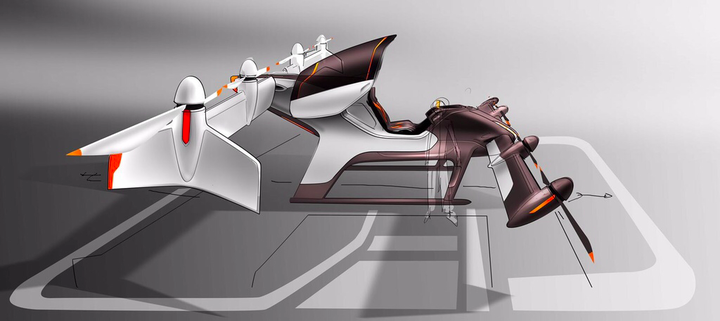
\includegraphics[width=\textwidth]{images/vahana_picture.png}
\caption{Vahana all-electric tandem tilt-wing with 8 rotors}
\label{fig:vahana}
\end{center}
\end{figure}

For the all-electric configuration, the input files are slightly different from the corresponding files for the conventional helicopter. An additional \red{Wings} dictionary is specified, and the propulsion architecture definition is also modified to reflect the new system. 
\subsection*{Input file 1: input.yaml}

\subsubsection{\red{Sizing}}
This dictionary specifies the values of high-level design variables to use for sizing the vehicle. For this vehicle type, \blue{Rotors}, \blue{Wings}, \blue{Fuselage}, \blue{Powerplant} and \blue{Transmission} are all defined and linked with the \red{Configuration} dictionary.

\paragraph{\blue{Rotors}}
The \blue{Rotor} sub-dictionary is shown below. Here, the number of inputs are far fewer than those required to size a helicopter rotor, for several reasons. The blade first flap natural frequency is not specified for eVTOLs, because rotor dynamics is no longer a key driver for blade sizing - sizing for strength automatically results in a very stiff design at the scales of interest. Additionally, neither disk loading nor rotor radius are specified, and so the wing-mounted rotors are automatically sized to ensure that the maximum possible disk area is achieved. Finally, the tip speed is markedly lower than that of a conventional helicopter's rotor, to reduce noise. This input value automatically guarantees that the advancing blade tip mach number in cruise is sufficiently low as to ensure almost zero compressibility drag. By not specifying the cruise rotor speed, a default value of 50\% hover tip speed is assigned. 

\begin{lstlisting}
   <@\blue{Rotors:}@>
      All_rotors:
      All_rotors:
         Nb:         [3]                      # per rotor
         Vtip:       [170]                    # hover tip speed, m/s
         ctsigma:    [0.139]
\end{lstlisting}
This definition shows that there is one rotor group used in the vehicle called `All\_rotors', with three design variables to size rotors in this group:
\begin{enumerate}
\item Number of blades per rotor \textbf{Nb} = 3
\item Tip speed \textbf{Vtip} = 170 m/s
\item Hover blade loading \textbf{ctsigma} = 0.139
\end{enumerate}
For the variable-RPM rotors used in eVTOLs, additional thrust can be achieved by changing the rotor speeds at the same blade loading. Therefore, the strict upper limits of $C_T/\sigma$ - usually observed in conventional helicopters with constant-speed rotors - can be relaxed for eVTOLs. 

\paragraph*{Rotor sizing rules}
If the rotor disk loading in hover is not specified (keyword \textbf{DL}, lb/sq.ft) and the rotor radius (keyword \textbf{radius}, meters) is also not specified, the rotor is assumed to be mounted on a wing, and the size is set based on wing span (calculated in fixed wing sizing) and rotor tip clearance (specified in \textbf{defaults.yaml}). After calculating rotor radius, the tip speed is used to identify the mean \textbf{rotor blade chord}. If the rotor geometric solidity (keyword \textbf{solidity}) is specified, then the hover blade loading is calculated. Otherwise, the the hover blade loading (keyword \textbf{ctsigma}) must be specified, and the geometric solidity is calculated. Some additional inputs are rotor cruise RPM to hover RPM ratio (keyword \textbf{RPM\_ratio}), and first flap frequency in hover (keyword \textbf{fl\_freq}). If these inputs are not specified, then default values of $\Omega_C/\Omega_H$ = 0.5 and $\nu_\beta$=1.1/rev are assumed. 

\paragraph{\blue{Wings}}
The \blue{Wings} dictionary consists of sub-dictionaries, with each sub-dictionary corresponding to a fixed wing group. Several instances of this fixed wing unit may exist on the vehicle; this detail is specified by the parameter \textbf{nwing}. In the example shown above, the \blue{Wings} dictionary is shown below, and the relevant keywords are summarized in Table~\ref{tbl:wing_keywords}.

\begin{lstlisting}
   <@\blue{Wings:}@>
      Main_wing:
         nwing:            [2]
         aspectratio:      [3,4,5,6,7,8] 
         cl:               [0.3,0.4,0.5,0.6,0.7]
         liftfraction:     [1]
         nrotors:          [4]
\end{lstlisting}

\begin{center}
  \begin{table}[H]
	\caption{Keywords for defining wing parameters}
	\label{tbl:wing_keywords}
    \begin{tabular}{| c | l | c |}
    \hline
    Keyword & Meaning & Value in example \\ 
    \hline
\textbf{nwing} & Number of fixed wings in this set &  2 \\
\textbf{aspectratio} & Wing geometric aspect ratio & [3, 4, ..] \\
\textbf{cl} & Wing lift coefficient in cruise & [0.3, 0.4, ..] \\
\textbf{liftfraction} & Weight fraction in cruise carried by this wing set & 1 \\
\textbf{nrotors} & Number of rotors mounted on each wing & 4 \\
     \hline
  \end{tabular}
\end{table}
\end{center}
\vspace{-1cm}

This input specifies one fixed wing group called ``Main\_wing'', of which there are \textbf{nwing}=2 identical units. The name ``Main\_wing'' is not a keyword - it is a character string that is used to refer to the set of wings defined using \textbf{keywords}, and build associations with rotor groups through the \red{Configuration} dictionary. The parameter \textbf{aspectratio} is the wing aspect ratio $b^2/S_{\rm wing}$, \textbf{cl} is the wing cruise lift coefficient and \textbf{liftfraction} is the fraction of vehicle weight carried by the the \textbf{nwing} units in this wing group during cruise. Finally, the parameter \textbf{nrotors} specifies the number of rotors mounted on a wing of this group. Here, 4 rotors are mounted on each wing in this group. Each input parameter can be specified as a single value or list of values to use for sizing.

\paragraph{\blue{Fuselage}}
The fuselage input dictionary for the tilt-wing is shown below. The dictionary specifies that the fuselage does not directly support any rotors, and that it is responsible for carrying no cruise lift. 
\begin{lstlisting}
   <@\blue{Fuselage:}@>
      nrotors:      [0]
      liftfraction: [0.0]
\end{lstlisting}

\paragraph{\blue{Powerplant}}
The source of power for the all-electric aircraft is a Lithium-ion battery, defined as shown below. The name \texttt{`BatteryPack'} is not a keyword - it is only the name of the powerplant group that supplies energy to the system. The keyword \textbf{type} is defined as `battery' to indicate the use of a Lithium-ion pack. The details for the battery cells and pack assembly are provided in \textbf{defaults.yaml}.

\begin{lstlisting}
   <@\blue{Powerplant:}@>
      BatteryPack: 
         type: `battery'
         num:  1
         redundancy: 0        
\end{lstlisting}

\paragraph{\blue{Transmission}}
In this aircraft, there is a single electric transmission, indicated by the keyword \textbf{type} defined as \texttt{`electric'} below. The transmission efficiency is 1, i.e., 100\% of the energy is transmitted without losses (usually 0.98, here shown as 1 for illustrative purposes). Additionally, motor efficiencies in hover and cruise are defined through the keywords \textbf{hover\_efficiency} and \textbf{cruise\_efficiency}. These keywords will be ignored if a higher-fidelity motor model is integrated into the sizing loop (future expansions).

\begin{lstlisting}
   <@\blue{Transmission:}@>
      ElTrans: 
         type:      `electric'
         eta:           1.00
         redundancy:    1.0   
         Motors:
            hover_efficiency: 0.90
            cruise_efficiency: 0.85
\end{lstlisting}

\paragraph{High-fidelity model switches}
The parameter \textbf{ifea} is a logical input, used to specify if the FEA-based weight model is to be used in the sizing loop to estimate the airframe structural weight. The other parameter \textbf{use\_bemt} indicates whether the Blade Element Momentum Theory (BEMT) should be used to refine rotor performance estimates in hover (and cruise for prop-rotors). In this example, both options are not enabled. 

\subsubsection{Aircraft \red{Configuration}}
The vehicle configuration details the association of rotors, wings, transmissions and powerplants. The \blue{Wings} dictionary shows that the wing group called `Main\_wing' supports rotors belonging to the group `All\_rotors'. The \blue{Rotors} dictionary shows that the rotor group `All\_rotors' draws power through the transmission group `ElTrans'. The \blue{Transmission} dictionary indicates that the transmission called `ElTrans' draws all of its power (\textbf{PowerFraction}=1.0) from `BatteryPack'. Each of these building blocks have been defined in the \red{Sizing} dictionary; the \red{Configuration} dictionary is used to create associations between these components. 

For electric transmissions, the analysis automatically sizes the drive motors based on all rotor groups that draw power through a given transmission.

\begin{lstlisting}
<@\textcolor{red}{\textbf{Configuration:}}@>
   <@\blue{Wings:}@>
      Main_wing:     `All_rotors'   # whichrotor group to mount on this wing 
   <@\blue{Rotors:}@>
      All_rotors:    `ElTrans'      # transmission used to power the rotors
   <@\blue{Transmission:}@>                   
      ElTrans:                        # transmission group name 
         Powerplant: `BatteryPack'  # connected powerplant group name
         PowerFraction: 1.0           # rated power fraction supplied 
\end{lstlisting}

\subsubsection*{Configuration mapping rules}
At present, multiple rotors from the same group may be mounted on wings or fuselages. One powerplant may supply energy to multiple transmissions, but  each rotor group may draw power from only one transmission group. However, one transmission group may supply power to multiple rotor groups. Work is ongoing to release advanced features with hybrid powerplants with heterogeneous power sources. 

\subsubsection{\red{Mission profile}}
The mission profile from \textbf{input.yaml} is show below. This input does not require any modification for all-electric vehicles, because it does not depend on the configuration.
\begin{lstlisting}
<@\textcolor{red}{\textbf{Mission:}}@>
   nsegments:          4
   flight_mode:        ['hover','cruise', 'cruise','hover'   ]
   time_seg:           [    1.5,       0,        0,    1.5   ]
   start_altitude:     [    0.0,    00.0,        0,      0   ] # m
   end_altitude:       [    0.0,     0.0,        0,      0   ] # m
   delta_temp_isa:     [    0.0,     0.0,        0,      0   ] # centrigrade
   rate_of_climb:      [      0,       0,        0,      0   ] # m/min
   cruise_speed:       [      0,      98,       98,      0   ] # knots
   distance:           [      0,      50,       15,      0   ] # in km
   add_payload:        [      0,       0,        0,      0   ] # dropped payload 
   segment_type:       [  `all',   `all',`reserve',   `all'  ] # 
   sizing_order:       [      1,       2,        0,      0   ] # order of sizing
\end{lstlisting}

\pagebreak
\subsubsection{\red{Aircraft}}

The aircraft specification dictionary is shown below. This input block also has identical keywords compared to the single main rotor helicopter, because it does not depend on the configuration (only the mission).

\begin{lstlisting}
<@\textcolor{red}{\textbf{Aircraft:}}@>
Aircraft:
   aircraftID: 2
   mass_payload:     345.0       # 250 kg payload + 70 kg margin
   mass_crew:         0 
   avionics:         79.2
   common_equipment: 24.0        # HVAC systems - common for all PAX
   common_per_pax:   00.0
   pax_count:         0          # number of passengers 
\end{lstlisting}

\subsection*{Input file 2: defaults.yaml}
This input file contains the sizing constraints, powerplant details, calibration factors for empirical/reduced-order weight and performance models and cost models. Also included are ``technology factors'', i.e., multipliers applied to weight predictions for each component. The file is too large to be printed verbatim as a whole unit; instead the text is subdivided into dictionary-sized chunks, and each dictionary in this input file is detailed below.

\subsubsection{\red{Sizing} dictionary}
\begin{lstlisting}
<@\red{Sizing:}@>
   <@\blue{Constraints:}@>
      max_rotor_radius:    14.01 # m
      max_ct_sigma    :     0.14
      max_gtow        :  5000.0 # kg
\end{lstlisting}

\blue{Constraints} used to size the vehicle are specified in this dictionary. The first parameter \textbf{max\_rotor\_radius} is the maximum rotor radius (for single main rotor helicopters) or the maximum vehicle footprint (for eVTOL). The parameter \textbf{max\_ct\_sigma} is the upper limit on rotor blade loading in hover. Finally, \textbf{max\_gtow} is the upper limit on take-off mass imposed for the vehicle. These constraints are imposed during optimization as well as iterative sizing. If any of these three constraints are violated during fixed-point iterations, the sizing loop is terminated and the design is marked ``invalid''.

\subsubsection{\red{Empirical} parameters}
This dictionary contains several sub-dictionaries, each of which are detailed below. A sample dictionary is broken into sub-dictionaries and explained below, and the keywords are summarized in Table~\ref{tbl:battery_keywords}.

\paragraph{\blue{Battery}}
The \blue{battery} sub-dictionary features parameters to model individual cells, as well as the battery pack. The cell parameters are \textbf{sp\_energy} (maximum rated energy stored per unit cell mass), \textbf{Tmax} (maximum rated cell temperature), \textbf{energy\_vol} (rated energy per unit cell volume) and \textbf{volume} (unit cell volume in liters).

\begin{lstlisting}
   <@\blue{Battery:}@>
      Cell:
         sp_energy:   240.0      # measured in W-hr/kg
         Tmax:         70.0      # max cell temperature, deg C
         energy_vol:  632.0      # energy density, Watt-hours/liter
         volume:        0.01708  # volume of a cell unit, liters
      Pack:
         SOH:           0.8      # state of health; 0 = gone; 1 = brand new
         DOD_min:       0.075    # minimum depth of discharge;
         integ_fac:     0.75     # battery pack integration factor for mass 
         vol_fac:       0.3      # battery volume integration factor 
      Force_sizing:     `energy' # ignore cell count or temperature effects      
\end{lstlisting}
The battery pack is quantified by the following parameters
\begin{enumerate}
\item State of health \textbf{SOH} - the maximum energy that can be stored in the pack, as a fraction of its rated energy. This parameter is usually less than unity because charge/discharge cycling of cells results in reduced energy storage capacity.
\item Minimum depth of discharge \textbf{DOD\_min} - the minimum energy capacity that the pack must retain to avoid permanent set and reduced energy capacity in individual cells. 
\item Pack mass integration factor \textbf{integ\_fac} - the ratio of battery cell mass to pack mass, to account for the battery casing and power management systems.
\item Pack volume factor \textbf{vol\_fac} - the ratio of cell mass to battery pack mass, to account for additional components introduced by the mass integration factor, as well as clearances for cell cooling.
\item Finally, the battery sizing option \textbf{Force\_sizing} is a string input that directs the battery sizing module to ignores thermal effects and pack voltage constraints; if this input is present, only energy-based sizing is performed.
\end{enumerate}

\begin{center}
  \begin{table}[H]
	\caption{Keywords for defining battery parameters}
	\label{tbl:battery_keywords}
    \begin{tabular}{| c | l | c |}
    \hline
    Keyword & Meaning & Value in example \\ 
    \hline
\textbf{Cell} & Indented entries pertain to cell properties &  -- \\
\textbf{sp\_energy} & Specific energy of a cell (Watt-hr/kg) &  -- \\
\textbf{Tmax} & Maximum cell temperature (deg C) & 70.0 \\
\textbf{energy\_vol} & Cell energy per unit volume (Watt-hr/liter) & 632.0 \\
\textbf{volume} & Volume of cell unit (liters) & 0.01708 \\
\textbf{Pack} & Indented entries pertain to pack properties &  \\
\textbf{SOH} & Average cell state of health (0 to 1) & 0.8 \\
\textbf{DOD\_min} & Minimum depth of discharge allowed (0 to 1) & 0.075 \\
\textbf{integ\_fac} & Mass of cells / mass of pack & 0.75 \\
\textbf{vol\_fac} & Volume of cells / volume of pack & 0.3 \\
\textbf{Force\_sizing} & String input to choose type of sizing & `energy' \\
     \hline
  \end{tabular}
\end{table}
\end{center}
\vspace{-1cm}

\paragraph{\blue{Aerodynamics}}
The \blue{aerodynamics} dictionary is used to specify rotor hover and cruise efficiencies, interference losses, wing efficiencies and body drag. A sample dictionary is shown below.

\begin{lstlisting}
   <@\blue{Aerodynamics:}@>
      Rotors:
         hover_dwld_factor:    0.015
         cd0:                  0.012
         induced_power_factor: 1.18
         FM:                   0.75
         kint:                 1.02
         hover_thrust:         `equal'
      Wings:
         oswald:            0.8
         cd0:               0.014
      Propellers:
         eta:               0.85
      Body:
         flat_plate_factor: 0.88       # means use drag build-up model
\end{lstlisting}

The sub-dictionaries for Rotors, Propellers and Body have been described in the previous section and are not repeated here. The empirical parameters used to model Wing performance are the Oswald efficiency factor \textbf{oswald} (quantifies additional induced drag for non-elliptical span loading) and the mean profile drag coefficient \textbf{cd0}, summarized in Table~\ref{tbl:wing_aero_keywords}. 

\begin{center}
  \begin{table}[H]
	\caption{Keywords for defining wing performance parameters}
	\label{tbl:wing_aero_keywords}
    \begin{tabular}{| c | l | c |}
    \hline
    Keyword & Meaning & Value in example \\ 
    \hline
\textbf{oswald} & Oswald efficiency factor &  0.8 \\
\textbf{cd0} &  Wing airfoil section profile drag coefficient & 0.014 \\
     \hline
  \end{tabular}
\end{table}
\end{center}
\vspace{-2cm}

\begin{center}
  \begin{table}[h]
	\caption{Keywords for defining geometric parameters}
	\label{tbl:geometry_keywords}
    \begin{tabular}{| c | l | c |}
    \hline
    Keyword & Meaning & Value in example \\ 
    \hline
\textbf{fuselage\_width} & Fuselage equivalent diameter (m) &  1.0 \\
\textbf{fuselage\_length} &  Fuselage length (m) & 7.0 \\
\textbf{clearance} &  Rotor tip clearance/radius & 7.0 \\
     \hline
  \end{tabular}
\end{table}
\end{center}
\vspace{-2cm}
\paragraph{\blue{Geometry}}
\begin{lstlisting}
   <@\blue{Geometry:}@>
      fuselage_width:    1.00          # fuselage width in meters
      fuselage_length:   7.00          # fuselage length in meters
      clearance:         0.15          # rotor tip clearance / radius ratio
\end{lstlisting}
The three geometry parameters used for sizing are the fuselage width at the widest point \textbf{fuselage\_width} (meters), airframe length \textbf{fuselage\_length} (meters) and the rotor clearance parameters \textbf{clearance}. This final parameter is the in-plane clearance between a rotor plane and other rotor planes/vehicle fuselage. The geometry parameters are summarized in Table~\ref{tbl:geometry_keywords}.

\paragraph{\blue{Technology factors}}
The term technology factor refers to scaling factors (``multipliers'') used to increase or decrease component empty weights to account for improvements in lightweight manufacturing. A sample dictionary is shown below. In the present case, the wing mass is scaled to 90\% of the predicted value, landing gear is scaled to 40\% of the model prediction and anti-icing group is neglected.
\begin{lstlisting}
   <@\blue{Tech\_factors:}@>
      Weight_scaling:
         wing:             0.9          # wings
         landing_gear:     0.4          #  
         anti_icing:       0.0          # ignored  
\end{lstlisting}

\subsubsection{\red{Acquisition} cost model}

There are two types of costs associated with the rotorcraft that are modeled in \hydra: acquisition cost (component purchase) and operating cost. The dictionary \red{Acquisition} contains three sub-dictionaries: \blue{Fixed\_cost},  \blue{Scaling\_cost} and \blue{Beta\_acq\_factors}. Each of these dictionaries is detailed below with examples.

\paragraph{\blue{Fixed acquisition cost}}
\begin{lstlisting}
<@\red{Acquisition:}@>
   <@\blue{Fixed\_cost:}@>
      sense_avoid:    189817.0            # USD 
      avionics:       145807.0            # USD
      interiors:       45152.0            # USD, air conditioning/heater/HUD
      testing:          6400.0            # USD 
\end{lstlisting}
This sub-dictionary contains inputs for the cost of vehicle components that do not vary with vehicle size. These groups include the sense and avoid system, avionics, interiors and component testing. The keywords for defining acquisition cost parameters are shown in Table~\ref{tbl:acq_cost_keywords}.

\begin{table}[h]
\begin{center}
	\caption{Keywords for defining acquisition cost parameters}
	\label{tbl:acq_cost_keywords}
    \begin{tabular}{| c | l | c |}
    \hline
    Keyword & Meaning & Value in example \\ 
    \hline
\textbf{sense\_avoid} & System purchase cost&  189817.0 \\
\textbf{avionics} & System purchase cost &  145807.0 \\
\textbf{interiors} & System purchase cost &  45152.0 \\
\textbf{testing} & System purchase cost &  6400.0 \\
     \hline
  \end{tabular}
\end{center}
\end{table}

\paragraph{\blue{Scaling\_cost}}
This sub-dictionary contains inputs for the cost of vehicle components that scale with the mass of each component. Several components fall under this category, particularly airframe, wings, landing gear, rotor blade structures, transmission lines and motors. A sample dictionary is shown below, and the relevant keywords are summarized in Table~\ref{tbl:scaling_cost_keywords}.

\begin{lstlisting}
   <@\blue{Scaling\_cost:}@>
      final_assem_line:    90.07          # USD/kg of take-off mass 
      BRS:                 10.885         # USD/kg of take-off mass 
      fuselage:          2807.0           # USD/kg of fuselage weight
      landing_gear:      1725.0           # USD/kg of landing gear strl.  weight
      wing_structure:    3779.1           # USD/kg of wing     structural weight
      motors:            2669.0           # USD/kg of drive motor mass 
      power_dist:          31.0           # USD/kW of installed power
      rotor_blade:      77605.0           # USD/sq.m of plan-form area
      rotor_hub:        14133.0           # USD/kg: hub+collective actuator
      wires:               20.3           # USD/kg of wire weight 
      tilt_actuator:     2868.0           # USD/kg of tilt actuator weight 
      wing_flap:         2619.0           # USD/kg of wing flap/aileron    
\end{lstlisting}

\begin{table}[h]
\begin{center}
	\caption{Keywords for defining cost elements that scale with vehicle properties}
	\label{tbl:scaling_cost_keywords}
    \begin{tabular}{| c | l | c |}
    \hline
    Keyword & Meaning & Value in example \\ 
    \hline
\textbf{final\_assem\_line} & Cost per kg of take-off mass &  90.07 \\
\textbf{BRS} & Cost per kg of emergency parachute mass &  10.885 \\
\textbf{fuselage} & Cost per kg of fuselage mass & 2807.0  \\
\textbf{landing\_gear} & Cost per kg of landing gear mass & 2807.0  \\
\textbf{motors} & Cost per kg of electric motor mass &   2669.0\\
\textbf{power\_dist} & Cost per kg of power distribution system mass & 31.0 \\
\textbf{rotor\_blade} & Cost per kg of rotor blade mass &  77605.0 \\
\textbf{rotor\_hub} & Cost per kg of rotor hub mass &  14133.0 \\
\textbf{wires} & Cost per kg of wire mass &  20.3\\
\textbf{tilt\_actuator} & Cost per kg of tilt actuator mass &  2868.0 \\
\textbf{wing\_flap} & Cost per kg of wing flaps mass &  2619.0 \\
     \hline
  \end{tabular}
\end{center}
\end{table}

\paragraph{\blue{Acquisition cost scaling factors}}
This dictionary deals with cost multipliers that account for reduction of component prices associated with mass-production. A value less than one indicates that the component is less expensive when manufactured in bulk or performed at large scales. The keywords to define these parameters are summarized in Table~\ref{tbl:cost_tech_factors}. 

\begin{lstlisting}
   <@\blue{Beta\_acq\_factors:}@>                    # acquisition cost multipliers 
      sense_avoid:         0.5            
      avionics:            0.75           
      interiors:           1.0            # air conditioning/heater/HUD
      testing:             1.0            
      final_assem_line:    0.5            
      BRS:                 0.75           
      fuselage:            0.2            
      landing_gear:        0.2            
      wing_structure:      0.2            
      motors:              0.2            
      power_dist:          1.0            
      rotor_blade:         0.2            
      rotor_hub:           0.2            
      wires:               1.0            
      tilt_actuators:      0.75           
      wing_flaps:          0.75           
\end{lstlisting}

\begin{table}[H]
\begin{center}
	\caption{Keywords for defining cost scaling factors}
	\label{tbl:cost_tech_factors}
    \begin{tabular}{| c | l | c |}
    \hline
    Keyword & Meaning & Value in example \\ 
    \hline
\textbf{sense\_avoid} & Cost multiplier for sense and avoid system & 0.5 \\
\textbf{avionics} & Cost multiplier for avionics &  0.75 \\
\textbf{interiors} & Cost multiplier for interiors &  1.0 \\
\textbf{testing} & Cost multiplier for final testing &  1.0 \\
\textbf{final\_assem\_line} & Cost multiplier for final assembly line &  0.5 \\
\textbf{BRS} & Cost multiplier for emergency parachute &  0.5 \\
\textbf{fuselage} & Cost multiplier for fuselage structure &  0.5 \\
\textbf{landing\_gear} & Cost multiplier for landing gear structure &  0.5 \\
\textbf{wing\_structure} & Cost multiplier for wing structure&  0.5 \\
\textbf{motors} & Cost multiplier for motors & 0.5 \\
\textbf{power\_dist} & Cost multiplier for power distribution systems &  0.5 \\
\textbf{rotor\_blade} & Cost multiplier for rotor blades &  0.2 \\
\textbf{rotor\_hub} & Cost multiplier for rotor hubs&  0.2 \\
\textbf{wires} & Costmultiplier for wires &  1.0 \\
\textbf{tilt\_actuator} & Cost multiplier for tilt actuators &  0.75 \\
\textbf{wing\_flap} & Cost multiplier for wing flaps &  0.75 \\
     \hline
  \end{tabular}
\end{center}
\end{table}

\subsubsection{\red{Operations}}
Operating costs are of two types: \blue{annual} and \blue{hourly} operating costs. These two components of the operating cost model are specified as sub-dictionaries under \red{Operations}. Additionally, the constants required to obtain \blue{battery} life cycle costs are also specified. Finally, \blue{vertiport} details are also specified and the cost of an eVTOL trip is compared to the cost of using a \blue{taxi} for traveling the same distance. Each of these sub-dictionaries are detailed below.

\paragraph{\blue{Annual} costs}
The sample \blue{Annual} operating cost inputs are shown below, and the relevant keywords are summarized in Table~\ref{tbl:annual_keywords}.
\begin{lstlisting}
<@\red{Operations:}@>
   <@\blue{Annual:}@>
      Flight_hours:        1500              # flight hours per year
      Liability:           22000             # USD liability insurance per year
      Inspection:          7700           # USD, per year
      Insurance_percent:   4.5               # insurance, % of acquisition 
      Depreciation_percent: 10               # % of acquisition cost depr./year
      Pilot:               280500            # USD, pilot cost to company/year
      Training:            9900              # USD, pilot training/year
\end{lstlisting}

The number of flight hours per year (\textbf{Flight\_hours}) is used to calculate the equivalent cost per flight hour from the annual fixed costs incurred in ensuring vehicle airworthiness. The annual costs incurred are \textbf{Liability}, \textbf{Inspection}, insurance and depreciation (specified as a percentage of acquisition cost, \textbf{Insurance\_percent} and \textbf{Depreciation\_percent} respectively). For a piloted vehicle, additional costs are incurred for pilot salary and overhead (\textbf{Pilot}) as well as continuous training (\textbf{Training}). 

\begin{table}[H]
\begin{center}
	\caption{Keywords for defining cost scaling factors}
	\label{tbl:annual_keywords}
    \begin{tabular}{| c | l | c |}
    \hline
    Keyword & Meaning & Value in example \\ 
    \hline
\textbf{Flight\_hours} & Flight hours operated per year & 1500 \\
\textbf{Liability} & Cost for liability insurance per year &  22000\\
\textbf{Inspection} & Cost for annual inspection &  7700\\
\textbf{Insurance\_percent} & Hull insurance as \% of acquisition cost &  4.5\\
\textbf{Depreciation\_percent} & Depreciation as \% of acquisition cost &  10\\
\textbf{Pilot} & Pilot annual salary and benefits &  280500\\
\textbf{Training} & Pilot annual training update cost &  9900\\
     \hline
  \end{tabular}
\end{center}
\end{table}
\vspace{-1cm}

\paragraph{\blue{Hourly} costs}
\noindent This dictionary specifies the maintenance and inspection costs associated with operating an air vehicle. A sample input chunk for \blue{Hourly} costs is shown below, and the keywords are summarized in Table~\ref{tbl:hourly_keywords}. The three elements in this dictionary are 
\begin{enumerate}
\item Frame inspection (\textbf{Frame\_maintenance}): specified as a cost in currency per flight hour
\item Rotor blades, collective actuator and hub inspection (\textbf{Rotor\_inspection}): specified as a cost in currency per flight hour per unit assembly
\item Electric motor inspection (\textbf{Motor\_inspection}): specified as a cost in currency per flight hour per motor unit.
\end{enumerate}

\begin{lstlisting}
   <@\blue{Hourly:}@>
      Frame_maintenance:     37.35           # $/flight hr 
      Rotor_inspection:       1.0            # $/flight hr/rotor 
      Motor_inspection:       0.625          # $/flight hr/rotor 
\end{lstlisting}

\begin{table}[H]
\begin{center}
	\caption{Keywords for defining maintenance costs incurred per flight hour}
	\label{tbl:hourly_keywords}
    \begin{tabular}{| c | l | c |}
    \hline
    Keyword & Meaning & Value in example \\ 
    \hline
\textbf{Frame\_maintenance} & Frame upkeep cost per flight hour &  37.35\\
\textbf{Rotor\_inspection} & Rotor inspection cost per flight hour&  1.0\\
\textbf{Motor\_inspection} & Motor inspection cost per flight hour &  0.625\\
     \hline
  \end{tabular}
\end{center}
\end{table}
\vspace{-1.5cm}
\paragraph{\blue{Battery} costs}
This dictionary specifies the number of charge/discharge \blue{Cycles} that a battery can withstand before its usable energy reduces to the threshold design state of health specified in \red{Sizing} $\rightarrow$ \blue{Battery} $\rightarrow$ Pack $\rightarrow$ \textbf{SOH}. Additionally, the purchase price of a battery pack as well as the battery recharge cost are specified as cost per unit rated energy/cost per unit of energy (\textbf{Cost\_per\_kwh}, \textbf{Electricity} respectively). The keywords for battery costs are summarized in Table~\ref{tbl:battery_cost_keywords}. In the present implementation, a charge/discharge cycle is assumed to correspond to one flight. Therefore, in the example input provided, the battery is replaced after 900 flights, regardless of the actual charge/discharge levels achieved.

\begin{lstlisting}
   <@\blue{Battery:}@>
      Cycles:             900
      Cost_per_kwh:       180.0              # battery cost/rated energy, $/kWh
      Electricity:          0.20             # electricity/unit energy, $/kWh
\end{lstlisting}

\begin{table}[H]
\begin{center}
	\caption{Keywords for defining battery costs incurred}
	\label{tbl:hourly_keywords}
    \begin{tabular}{| c | l | c |}
    \hline
    Keyword & Meaning & Value in example \\ 
    \hline
\textbf{Cycles} & Number of charge/discharge cycles &  900 \\
\textbf{Cost\_per\_kwh} & Battery purchase cost/unit energy (kWh) capacity &  180.0\\
\textbf{Electricity} & Electricity cost/stored energy (kWh) for recharging &  0.2\\
     \hline
  \end{tabular}
\end{center}
\end{table}
\vspace{-1.5cm}
\paragraph{\blue{Vertiport}}
The relevant operational details at the vertiport are the landing tariffs (\textbf{Landing\_fees}) per touchdown, the distance from the vertiport to the final passenger destination (\textbf{Ground\_distance} in km) and the additional time spent in commuting to and from the vertiport changing modes of transport (\textbf{Padding\_time}).

\begin{lstlisting}
   <@\blue{Vertiport:}@>
      Landing_fees:        20.0              # landing fee per flight, USD
      Padding_time:        26.0              # min, curb -> UAM + UAM -> curb 
      Ground_distance:      2.0              # last leg distance in km
\end{lstlisting}

\begin{table}[H]
\begin{center}
	\caption{Keywords for defining vertiport-related operation parameters}
	\label{tbl:vertiport_keywords}
    \begin{tabular}{| c | l | c |}
    \hline
    Keyword & Meaning & Value in example \\ 
    \hline
\textbf{Landing\_fees} & Cost per landing &  20.0 \\
\textbf{Padding\_time} & Door $\rightarrow$ door time minus air time (min) &  20.0 \\
\textbf{Ground\_distance} & Door $\rightarrow$ door trip minus VTOL range (km) &  2.0 \\
\hline
  \end{tabular}
\end{center}
\end{table}

\begin{table}[H]
\begin{center}
	\caption{Keywords for defining taxi-related operation parameters}
	\label{tbl:taxi_keywords}
    \begin{tabular}{| c | l | c |}
    \hline
    Keyword & Meaning & Value in example \\ 
    \hline
\textbf{Distance\_rate} & Tariff per ground distance covered (km) &  0.55 \\
\textbf{Time\_rate} & Tariff per minute spent in taxi &  0.36 \\
\textbf{Padding\_time} & Door $\rightarrow$ door time minus time in taxi (min) &  15.0 \\
\hline
  \end{tabular}
\end{center}
\end{table}
\vspace{-1.5cm}
\paragraph{\blue{Taxi} details}
The details of a \blue{taxi} that can compete with a short-range aircraft are the tariff per unit distance traveled (\textbf{Distance\_rate} in currency per km), a time tariff (\textbf{Time\_rate} in currency per minute) and the additional time required to change from another mode of transport to the taxi (\textbf{Padding\_time}, minutes). The keywords for the \blue{Taxi} are summarized in Table~\ref{tbl:taxi_keywords}.
\begin{lstlisting}
   <@\blue{Taxi:}@>
      Distance_rate:        0.55             # Taxi price in USD per km 
      Time_rate:            0.36             # USD/minute of taxi ride
      Padding_time:        15.0              # airport gate to curb, minutes
\end{lstlisting}


\subsubsection{\red{Redundant} systems}
The dictionary \red{Redundancies} specifies components that feature doubly or triply redundant backups for flight controls, power cables and avionics. The redundancy factors are used to proportionally increase the component empty weights and associated group costs. The keywords for system redundancies are summarized in Table~\ref{tbl:redund_keywords}.

\begin{lstlisting}
<@\red{Redundancies:}@>
   wing_flap:              1.0 
   tilt_actuator:          2.0
   wires:                  1.0
   avionics:               1.0
\end{lstlisting}

\begin{table}[H]
\begin{center}
	\caption{Keywords for defining aircraft redundancy parameters}
	\label{tbl:redund_keywords}
    \begin{tabular}{| c | l | c |}
    \hline
    Keyword & Meaning & Value in example \\ 
    \hline
\textbf{wing\_flap} & Number of actuators per wing flap &  1.0 \\
\textbf{tilt\_actuator} & Number of actuators per wing/rotor tilt hinge &  2.0 \\
\textbf{wires} & Number of redundant power cables, signal wires &  1.0 \\
\textbf{avionics} & Number of redundant systems for avionics &  1.0 \\
\hline
  \end{tabular}
\end{center}
\end{table} 						% Input files
%\section{Output files}
This section of the documentation details the output file generated at the end of sizing. The file pattern is \textbf{log<XYZ>.yaml}, where <XYZ> is an integer representing a unique design ID number. The output is in plain text formatted as a YAML file, similar to the input files. These files can be read an automatically converted to \python \spc dictionaries using the \textbf{pyyaml} package. All outputs are stored under the \textbf{outputs/log/} subdirectory in the run folder.

\subsection{\textbf{log<XYZ>.yaml}}
An example output log file is detailed dictionary-by-dictionary below, and the relevant outputs are explained. 

\subsubsection{\red{vehicle} summary}
\begin{lstlisting}
# ---------------------------------------------------
# Mission and Vehicle Log
# ---------------------------------------------------
<@\red{vehicle:}@>
   aircraftID:               2 
   take_off_mass:            1734.67 # [kg]
   power_installed:          963.0 # [kW]
   Cruise_LbyD:              11.80 # 
\end{lstlisting}
The \red{vehicle} dictionary contains four high-level vehicle metrics. The \textbf{aircraftID} is an outdated output, that is a copy of the input value given in \textbf{input.yaml}. The other metrics given in this dictionary are the take-off mass in kg, sum of maximum rated motor power values in kiloWatts and the vehicle lift-to-drag ratio in the cruise sizing segment. 

\subsubsection{\red{Rotor}}
The \red{Rotor} dictionary provides details of the rotor geometry and performance in the hover sizing segment. Each sub-dictionary under the rotor dictionary corresponds to a unique rotor group. For each rotor group, the following outputs are specified:
\begin{enumerate}
\item \textbf{nrotor}: number of rotors of this type in the vehicle 
\item \textbf{nblade}: number of blades per rotor in this rotor type 
\item \textbf{disk\_loading}: rotor hover disk loading in pounds per square foot
\item \textbf{aspect\_ratio}: blade aspect ratio (radius to chord ratio)
\item \textbf{radius}: rotor radius in meters
\item \textbf{chord}: mean rotor blade chord in meters 
\item \textbf{tip\_speed}: rotor hover tip speed in m/s 
\item \textbf{hover\_FM}: rotor figure of merit in the hover sizing segment 
\item \textbf{cruise\_rpm\_ratio}: rotor cruise RPM divided by rotor hover RPM 
\item \textbf{eta\_xmsn}: transmission efficiency, 0 to 1  
\item \textbf{solidity}: rotor geometric solidity  
\item \textbf{cd0}: rotor blade airfoil drag coefficient at zero lift
\item \textbf{ipf}: rotor induced power factor in hover (non-ideal losses)
\item \textbf{hvr\_dwld}: hover download divided by rotor lift share 
\item \textbf{hvr\_ct\_sigma}: rotor blade loading in hover sizing segment 
\item \textbf{prop\_eta}: prop-rotor efficiency in cruise sizing segment
\end{enumerate}

\begin{lstlisting}
<@\red{Rotor:}@>
   <@\blue{set0:}@>
      nrotor:              8 
      nblade:              3 
      disk_loading:        16.76 # [lb/ft2]
      aspect_ratio:        5.86 
      radius:              0.93 # [m]
      chord:               0.158 # [m]
      tip_speed:           170.0 # [m/s]
      hover_FM:            0.750 
      cruise_rpm_ratio:    0.500 
      eta_xmsn:            1.000 
      solidity:            0.16299 
      cd0:                 0.012 
      ipf:                 1.234 
      hvr_dwld:            0.015
      hvr_ct_sigma:        0.139
      prop_eta:            0.850
\end{lstlisting}

\subsubsection{\red{Wings}}
This dictionary contains details of the wing geometry and operating condition in the cruise sizing segment. If multiple wing groups are present in the system, then details of each wing group are listed as sub-dictionaries. For each wing group, the following details are written:
\begin{enumerate}
\item \textbf{nwing}: the number of fixed wings of this type present in the vehicle.
\item \textbf{span}: the tip-to-tip dimension in meters
\item \textbf{chord}: the average wing chord in meters
\item \textbf{structure\_wt}: the weight of the structure for one wing
\item \textbf{wires\_wt}: the weight of wires running along one wing
\item \textbf{aspect\_ratio}: the wing aspect ratio 
\item \textbf{oswald}: the wing Oswald efficiency
\item \textbf{cd0}: the wing profile drag coefficient
\item \textbf{cl}: the operating lift coefficient for the cruise sizing segment
\item \textbf{lift\_fraction}: lift fraction for this wing group in the cruise sizing segment 
\item \textbf{rotors\_per\_wing}: the number of rotors mounted along a wing of this group
\item \textbf{rotor\_group\_id}: the group identifier for rotors mounted on this wing
\end{enumerate}
\begin{lstlisting}
<@\red{Wings:}@>
   <@\blue{set0:}@>
      nwing:               1 
      span:                11.086 # [m]
      chord:               2.217 # [m]
      structure_wt:        117.303 # [kg, each] 
      wires_wt:            66.506 # [kg, each] 
      aspect_ratio:        5.000 
      oswald:              0.800 
      cd0:                 0.014 
      cl:                  0.400 
      lift_fraction:       0.900 
      rotors_per_wing:       6 
      rotor_group_id:        0
   <@\blue{set1:}@>
      nwing:               1 
      span:                4.674 # [m]
	 ... (pattern repeats)
	 ...
\end{lstlisting}

\subsubsection{\red{Costs}}
The \red{costs} dictionary contains a breakdown of the vehicle acquisition cost and operating cost per flight hour, as well as the results of comparisons with a ground taxi. The individual sub-dictionaries are detailed below.
\paragraph{Acquisition cost breakdown}
The first row \textbf{Frame\_acquisition} is the acquisition cost of the aircraft in millions of currency. The following dictionary shows two values per line: the first value is the cost of the component in currency, and the second column shows the fraction of the component's acquisition cost as a percentage of the total acquisition cost.
\begin{lstlisting}
<@\red{Costs:}@>
   Frame_acquisition:   [0.779632] # [Millions of USD]
   <@\blue{acquisition\_cost\_breakdown:}@>
      BRS             : [      14161.395  ,  1.816] # [USD, % acquisition cost]
      avionics        : [     109355.250  , 14.027] # [USD, % acquisition cost]
      final_assem_line: [      42876.657  ,  5.500] # [USD, % acquisition cost]
      fuselage        : [      47190.123  ,  6.053] # [USD, % acquisition cost]
      interiors       : [      45152.000  ,  5.791] # [USD, % acquisition cost]
      landing_gear    : [      20874.300  ,  2.677] # [USD, % acquisition cost]
      motors          : [     117455.191  , 15.065] # [USD, % acquisition cost]
      power_dist      : [      29854.461  ,  3.829] # [USD, % acquisition cost]
      rotor_blade     : [      54432.887  ,  6.982] # [USD, % acquisition cost]
      rotor_hub       : [      20923.226  ,  2.684] # [USD, % acquisition cost]
      sense_avoid     : [      94908.500  , 12.174] # [USD, % acquisition cost]
      testing         : [       6400.000  ,  0.821] # [USD, % acquisition cost]
      tilt_actuators  : [      37893.206  ,  4.860] # [USD, % acquisition cost]
      wing_flaps      : [      29202.352  ,  3.746] # [USD, % acquisition cost]
      wing_structure  : [     106832.064  , 13.703] # [USD, % acquisition cost]
      wires           : [       2120.209  ,  0.272] # [USD, % acquisition cost]
\end{lstlisting}

\paragraph{\blue{Annual operating costs}}
This dictionary details the breakdown of annual operating costs for maintaining airworthiness. The field \textbf{Fixed\_operating\_costs} shows the aggregated annual costs in currency. The \blue{fixed cost breakdown} dictionary is organized in a manner similar to the previous section: the first column shows the cost in currency, and the second column shows the cost as a percentage of the annual cost. 

\begin{lstlisting}
   Fixed_operating_costs: [142746.614190] # [USD]
   <@\blue{fixed\_cost\_breakdown:}@>
      depreciation    : [      77963.182    , 54.616] # [USD, % fixed cost]
      inspection      : [       7700.000    ,  5.394] # [USD, % fixed cost]
      insurance       : [      35083.432    , 24.577] # [USD, % fixed cost]
      liability       : [      22000.000    , 15.412] # [USD, % fixed cost]
\end{lstlisting}

\paragraph{\blue{Variable operating costs}}
This section details the costs that depend on the number of flight hours that the vehicle is operated for. The field \textbf{Variable\_operating\_costs} details the currency spent per flight hour in operating costs due to maintenance, energy usage and inspections/cleaning. The variable operating costs are broken down into the individual cost elements in the \blue{variable\_cost\_breakdown} dictionary. The first number in the two-column rows is the cost in currency per flight hour, and the second number is the cost of that contributing element expressed as a percentage of the \textbf{Variable\_operating\_costs} field.

\begin{lstlisting}
   Variable_operating_costs: [290.210] # [USD/hr]
   <@\blue{variable\_cost\_breakdown:}@>
      battery_use     : [         51.327  , 17.686] # [USD/hr, % variable cost]
      electricity     : [         31.895  , 10.990] # [USD/hr, % variable cost]
      fixed_annual    : [         95.164  , 32.792] # [USD/hr, % variable cost]
      frame_overhaul  : [         37.350  , 12.870] # [USD/hr, % variable cost]
      landing_fees    : [         61.474  , 21.183] # [USD/hr, % variable cost]
      vpf_overhaul    : [         13.000  ,  4.480] # [USD/hr, % variable cost]
   UAM_time:            [         62.589] # [minutes    ]
   Taxi_time:           [         80.261] # [minutes    ]
   UAM_trip_cost:       [        101.662] # [USD        ]
   Taxi_trip_cost:      [         50.994] # [USD        ]
   Time_value:          [          2.867] # [$/min saved]
\end{lstlisting}

The last five fields are miscellaneous data that compare the performance and cost of an eVTOL with a ground taxi. \textbf{UAM\_time} is the time taken to travel from an airport gate to a vertiport, fly to another vertiport and finally travel the last leg by ground taxi (i.e., door-to-door time from airport to final destination through an ``air taxi''). The field \textbf{Taxi\_time} is the door-to-door time from airport to final destination using ground transport only. \textbf{UAM\_trip\_cost} is the total cost of operating a combined air taxi and ground taxi for the final leg, and the corresponding cost for the ground taxi-only option is \textbf{Taxi\_time\_cost}. The time value is defined as the price difference between the two transport options, divided by the time difference, or \textit{time value}.

\subsubsection{\red{Weight breakdown}}
This dictionary details the breakdown of vehicle weights. Three main weight categories are listed: \textbf{battery} (and/or \textbf{fuel}), \textbf{payload} and \blue{empty mass}. For rows with two columns, the first column is the component mass in kg, and the second column is the mass of the component expressed as a percentage of take-off mass. For rows with a single column, the number corresponds to a component's mass in kg.

For the \blue{empty weight} dictionary, each components is listed under sub-dictionaries. If the empty weight group is a dictionary with additional breakdowns within the component, those details are also printed, along with a field called \textbf{total} - the accumulated mass of components within that group. These breakdowns are plotted in pie charts by the postprocessing script \textbf{piethon.py}.
 
\begin{lstlisting}
<@\red{Weights:}@>
   <@\blue{empty\_weight:}@>
      total:            [ 952.1         ,  54.9] # [kg, %GTOW]
      alighting_gear  :
         total        : [  60.5         ,   3.5] # [kg, % GTOW]
         fairing      : [  26.0] # [kg]
         structure    : [  34.5] # [kg]
      avionics        : [  79.2         ,   4.6] # [kg, %GTOW]
      common_equip    : [  24.0         ,   1.4] # [kg, %GTOW]
      emergency_sys   : [  40.4         ,   2.3] # [kg, %GTOW]
      empennage       :
         total        : [  23.9         ,   1.4] # [kg, % GTOW]
         vtail        : [  23.9] # [kg]
      fuselage        :
         total        : [  84.1         ,   4.8] # [kg, % GTOW]
         bulkhead     : [  12.4] # [kg]
         canopy       : [  12.2] # [kg]
         keel         : [  14.9] # [kg]
         skin         : [  44.6] # [kg]
      powerplant      :
         total        : [ 220.0         ,  12.7] # [kg, % GTOW]
         motor_group0 : [ 220.0] # [kg]
      rotor           :
         total        : [ 143.6         ,   8.3] # [kg, % GTOW]
         group0actuatr: [  26.9] # [kg]
         group0blades : [  73.7] # [kg]
         group0hub    : [  43.0] # [kg]
      wing            :
         total        : [ 171.9         ,   9.9] # [kg, % GTOW]
         actuators    : [  14.9] # [kg]
         mounts       : [  22.0] # [kg]
         structure    : [ 117.4] # [kg]
         tilters      : [  17.6] # [kg]
      wires           :
         total        : [ 104.4         ,   6.0] # [kg, % GTOW]
         power_wire   : [  74.3] # [kg]
         signal_wire  : [  30.1] # [kg]
   battery:             [462.58         ,  26.7] # [kg]
   payload:             [320.02         ,  18.4] # [kg]
\end{lstlisting}

\subsubsection{\red{Volumes}}
The volume output section is under development, and additional fields will be introduced in future versions of \hydra. At present, the dictionary contains:
\begin{lstlisting}
<@\red{Volumes:}@>
   fuselage_width:            1.00 # [m]
   passenger_count:              0 # [people]
   battery_volume:           0.439 # [cu.m]
\end{lstlisting}
This dictionary outputs the fuselage width (specified in \textbf{defaults.yaml}) in meters, number of passengers (specified in \textbf{input.yaml}) and the calculated battery volume in cubic meters. 

\subsubsection{\red{Parasitic drag}}
This dictionary details the vehicle flat plate area (\textbf{flat\_plate\_area}) in square meters. If the (\red{Empirical} $\rightarrow$ \blue{Aerodynamics} $\rightarrow$ \textbf{Body} $\rightarrow$ flat\_plate\_factor input in \textbf{defaults.yaml} is set to zero, the component drag build-up for the vehicle parasitic drag is also printed in a sub-dictionary, \blue{flat\_plate\_breakdown}. The entries in this sub-dictionary are the parasitic drag of each component expressed as a percentage of the total flat plate area. 
\begin{lstlisting}
<@\red{Parasitic\_drag:}@>
   flat_plate_area:     0.422 # [sq.m] 
   <@\blue{flat\_plate\_breakdown:}@> 
      LG              : [ 41.0] # [%]
      base            : [  7.0] # [%]
      fus             : [ 18.9] # [%]
      prot            : [  9.1] # [%]
      spin            : [ 20.1] # [%]
      vt              : [  3.8] # [%]
\end{lstlisting}

\subsubsection{\red{Mission details}}
This dictionary provides relevant details for the vehicle performance during various mission segments. The field \textbf{total\_energy} is the energy in kWh required to complete the mission, which has \textbf{nsegments} segments. The segment types are given in the list \textbf{flight\_mode}, with the segment altitudes given in meters by the fields \textbf{start\_alt} and \textbf{end\_alt}. The variable \textbf{delta\_temp\_ISA} is the temperature offset at sea level for the sizing mission relative to the temperature in the International Standard Atmosphere model. The segment rate of climb is specified in feet per minute, while cruise speed is specified in knots. Segment duration is specified by the field \textbf{time}, and \textbf{rotor power required} for each segment is listed in kilowatts. The corresponding \textbf{battery power draw} is also listed in kW, and the battery \textbf{C-rating} is listed in 1/hr. The \textbf{cell temperature} (if the model is used in sizing) is shown at the end of each segment in deg C. Ambient \textbf{density} is specified in kg/cu.m. The vehicle mass at the beginning of each segment is listed in \textbf{segment\_mass}. The variable \textbf{segment\_type} is a character string; `all' indicates the segment is used for sizing and regular operations for operating cost evaluation; `reserve' indicates the segment is used for sizing only, but not for regular mission operating cost. The ground distance covered by the vehicle in kilometers is output in the field \textbf{segment\_distance}.
\begin{lstlisting}
<@\red{Mission:}@>
   total_energy:        67.07 # [kW-hr]
   nsegments:           4 
   flight_mode:         ['hover   ','cruise  ','cruise  ','hover   '] 
   start_alt:           [         0 ,         0 ,         0 ,         0 ] #[m]
   end_alt:             [         0 ,         0 ,         0 ,         0 ] #[m]
   delta_temp_ISA:      [      0.00 ,      0.00 ,      0.00 ,      0.00 ] #[C]
   rate_of_climb:       [         0 ,         0 ,         0 ,         0] #[ft/min]
   cruise_speed:        [      0.00 ,     98.00 ,     98.00 ,      0.00 ] #[knots]
   time:                [      1.50 ,     16.53 ,      4.96 ,      1.50 ] #[min]
   rotor_power_reqd:    [    486.76 ,    123.49 ,    123.49 ,    486.76 ] #[kW]
   battery_power_draw:  [    540.84 ,    145.28 ,    145.28 ,    540.84 ] #[kW]
   C-rating:            [      4.96 ,      1.33 ,      1.33 ,      4.96 ] #[1/hr]
   cell temperature:    [      0.00 ,      0.00 ,      0.00 ,      0.00 ] #[deg C]
   density:             [   1.226 ,     1.226 ,     1.226 ,     1.226] #[kg/cu.m]
   segment_mass:        [    2000.9 ,    2000.9 ,    2000.9 ,    2000.9 ] #[kg]
   segment_type:        ['all      ','all      ','reserve  ','all      ']
   segment_distance:    [       0.00,      50.00,      15.00,       0.00]
\end{lstlisting}

\subsubsection{\red{Battery details}}
This dictionary is used to output the details pertaining to the \red{battery}. The \textbf{rated\_capacity} is the rated energy in kWh of all vehicle battery packs. The \textbf{state\_of\_health} is the multiplier for the battery pack rated energy; the product of these two numbers is the maximum energy that the pack can store at the pack's end-of-life after several charge/discharge cycles. The parameter \textbf{depth\_discharge} is a fraction ranging from 0 to 1, which indicates the smallest energy fraction that the battery can be discharged to, without damaging the cells. In this example, the battery rated capacity before cycling is 109.07 kWh, and the design state of health is 0.8, i.e., at end of life, the maximum energy that can be stored in the battery is 0.8 $\times$ 109.07 = 87.25 kWh. The minimum depth of discharge is 0.075, i.e., the battery can be discharged until 0.075 $\times$ 109.07 = 8.18 kWh of energy is remaining, without permanently damaging the cells. 
\begin{lstlisting}
<@\red{Battery:}@>
   rated_capacity:      109.07 
   state_of_health:     0.800 
   depth_discharge:     0.075 
\end{lstlisting}
\subsection{\textbf{log<XYZ>.txt}}
The other output generated by \hydra \spc is the final converged design and its details stored as a \textbf{pickle} module. The various postprocessing scripts in \hydra \spc load the vehicle class in its converged state for various sensitivity studies and to extract details. To load the file corresponding to design ID = 0, use this template:\\
\textbf{import pickle} \\
\textbf{fname     = `outputs/log/log0.yaml'} \\
\textbf{with open(fname,`rb') as f:} \\
\textbf{$\textrm{          }$ $\textrm{    }$ design    = pickle.load(f)} \\
The variable \textbf{design} is an instance of the \textbf{hydraInterface} class with all methods and variables required to perform sizing.

\begin{landscape}
\subsection{\textbf{summary.dat}}
A high-level summary of all designs is provided in \textbf{summary.dat}. The first column is the unique design identifier; the second column is the take-off mass in kg, the third column is the installed power in kW, the fourth column is the mass sum of configuration fuel and battery (kg); the fifth column is the empty mass in kg; the sixth column is the payload mass in kg; the seventh column is the vehicle operating cost in currency per flight hour; the final column is an integer - 0 indicates the design is invalid, while 1 indicates the design satisfies all the constraints.
\begin{lstlisting}
  Design ID #      Weight (kg)     Power (kW)  Fuel/Batt (kg)   Empty Wt (kg)    Payload (kg) Op Cost ($/hr)   Valid design  
              0    1734.67         963.05          462.579        952.07          320.02         290.21050          1       
              1    1872.70         1171.23         525.369        1027.33         320.00         305.44722          1       
              2    2049.93         1411.57         609.178        1120.75         320.00         325.62067          1       
              3    1607.40         810.49          399.572        887.79          320.04         275.44891          1       
              4    1702.75         967.71          441.230        941.50          320.02         285.65621          1       
              5    1826.42         1143.83         497.869        1008.55         320.00         299.42785          1       
 ... 
\end{lstlisting}
\end{landscape}
 					% Output files
%\section{Running \hydra}
\begin{enumerate}
\item Create a run directory under \textbf{cases/}
\item Create input files \textbf{input.yaml}, \textbf{defaults.yaml}. If multiple input values of each design parameter are specified, the analysis generates all possible combinations of all specified design parameters, and launches multiple sizing operations.
\item Run sizing on a parametric sweep: copy \textbf{xrun.py} from a sample run directory to the current run folder, then use the following command:
\begin{center}
\textbf{python3 xrun.py} (serial mode)\\
\textbf{mpirun -n 8 python3 xrun.py} (parallel mode, 8 threads)
\end{center}
The various cases are automatically subdivided by \hydra \spc, analyzed and the summaries are collated in the summary.dat output file.
\item Sort valid designs: use the routine process\_data.py routine:
\begin{center}
\textbf{python3 process\_data.py}
\end{center}
This command will generate a file called \textbf{best\_design.dat} in the same format as summary.dat, with valid designs ranked in order of ascending cost, take-off weight, installed power, or empty weight depending on the user-specified choice in process\_data.py.
\end{enumerate}

\section{Postprocessing}
Several postprocessing scripts are provided in the \textbf{Postprocessing/} folder in the sample run directories. Copy these scripts to the run directory with results to postprocess. Examples of these commands and sample outputs are shown below:
\begin{enumerate}
\item \textbf{Pie chart generator}: the script \textbf{piethon.py} generates pie charts for the breakdown of empty weight, annual operating costs, hourly operating costs and parasitic drag. Invoke it using the command \\
\textbf{python3 Postprocessing/piethon.py <XYZ>} \\
Here, <XYZ> is the integer unique identifier for a design. For example,  the command \textbf{python3 Postprocessing/piethon.py 10} generates pie charts for a vehicle with the design ID 10. The relevant images are compiled into a PDF called \textbf{costs\_design\_10.pdf} for the sample input.  The individual pie charts are shown in Fig.~\ref{fig:pies}

\begin{figure}
     \centering
	\subfigure[Acquisition cost]{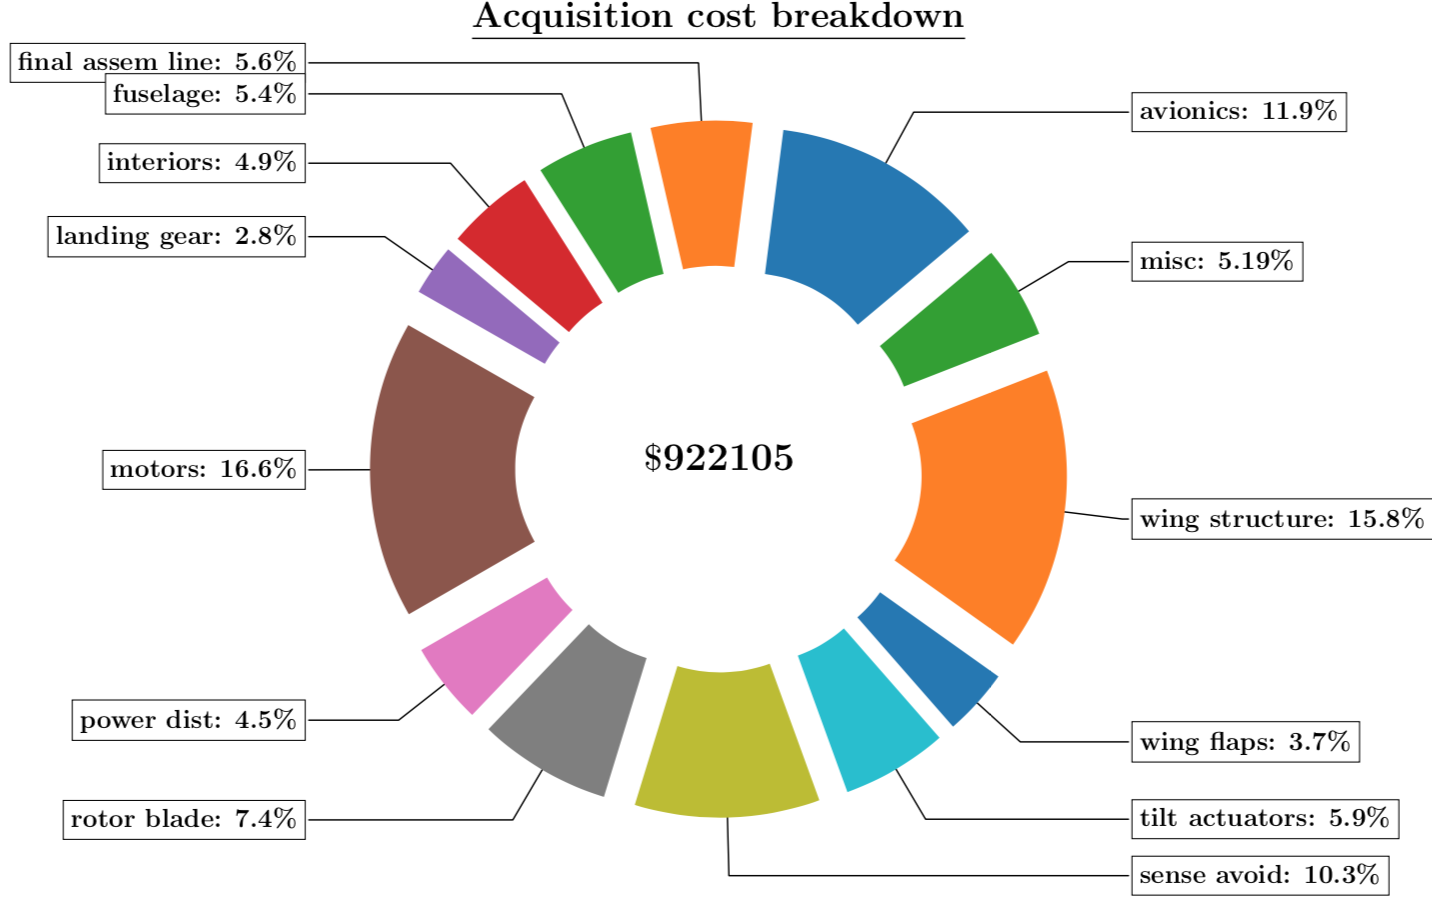
\includegraphics[width=0.45\textwidth]{images/pie3.png}}
	\subfigure[Annual cost]{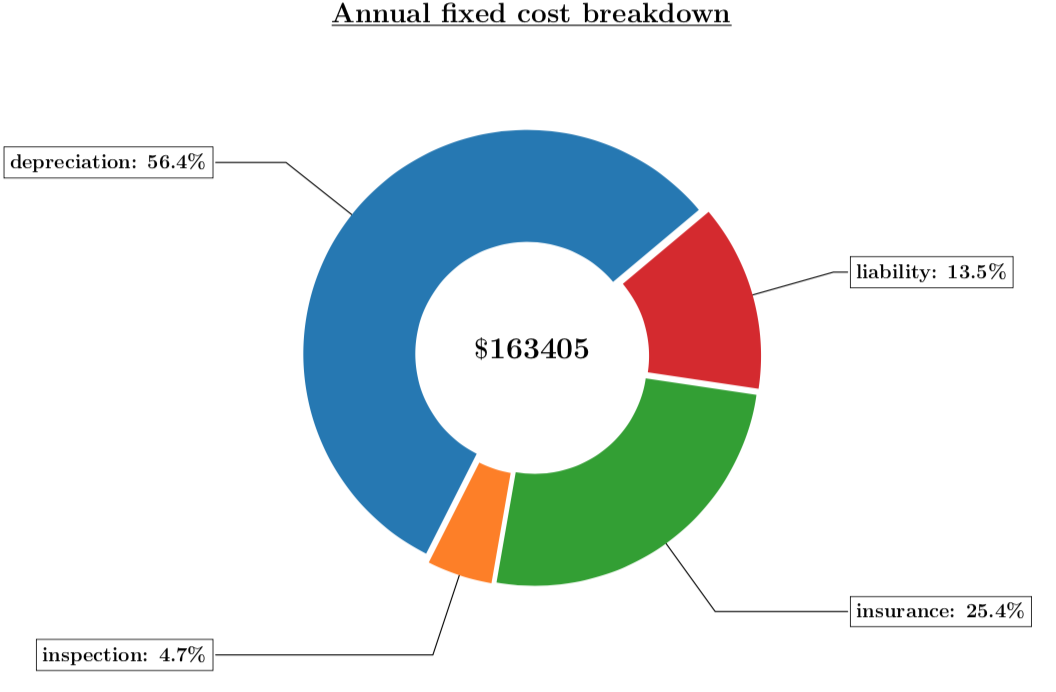
\includegraphics[width=0.45\textwidth]{images/pie5.png}}
	\subfigure[Operating cost]{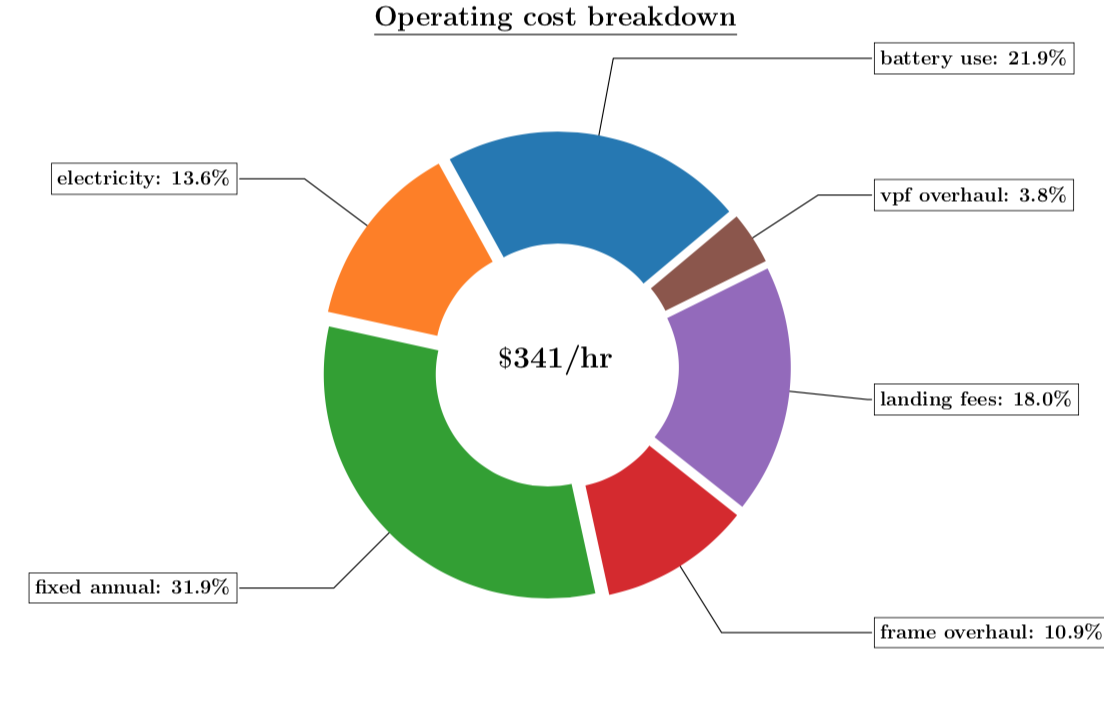
\includegraphics[width=0.45\textwidth]{images/pie2.png}}
	\subfigure[Parasitic drag breakdown]{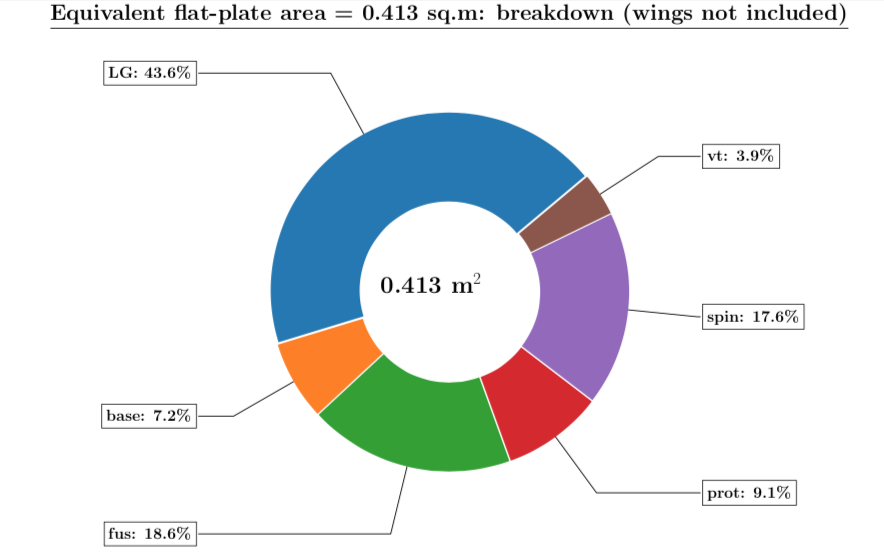
\includegraphics[width=0.45\textwidth]{images/pie1.png}}
	\subfigure[Vehicle weight]{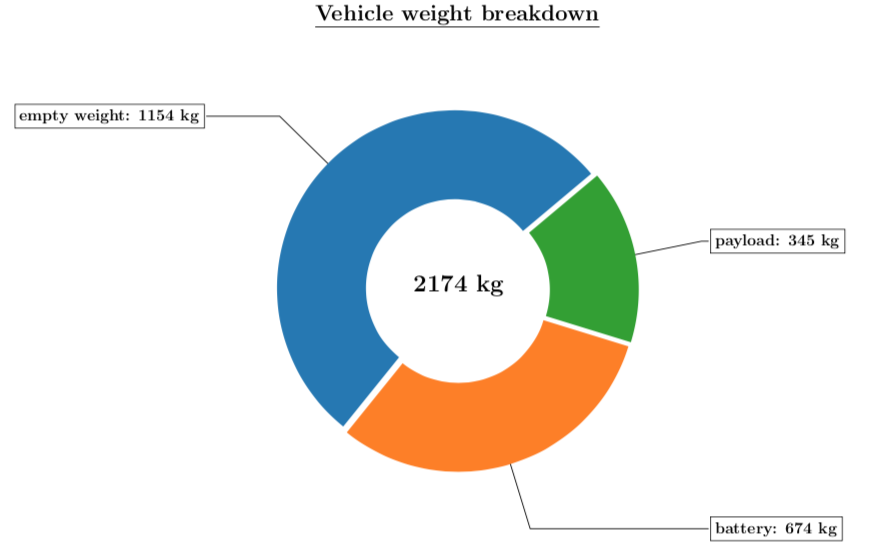
\includegraphics[width=0.45\textwidth]{images/pie6.png}}
	\subfigure[Empty weight]{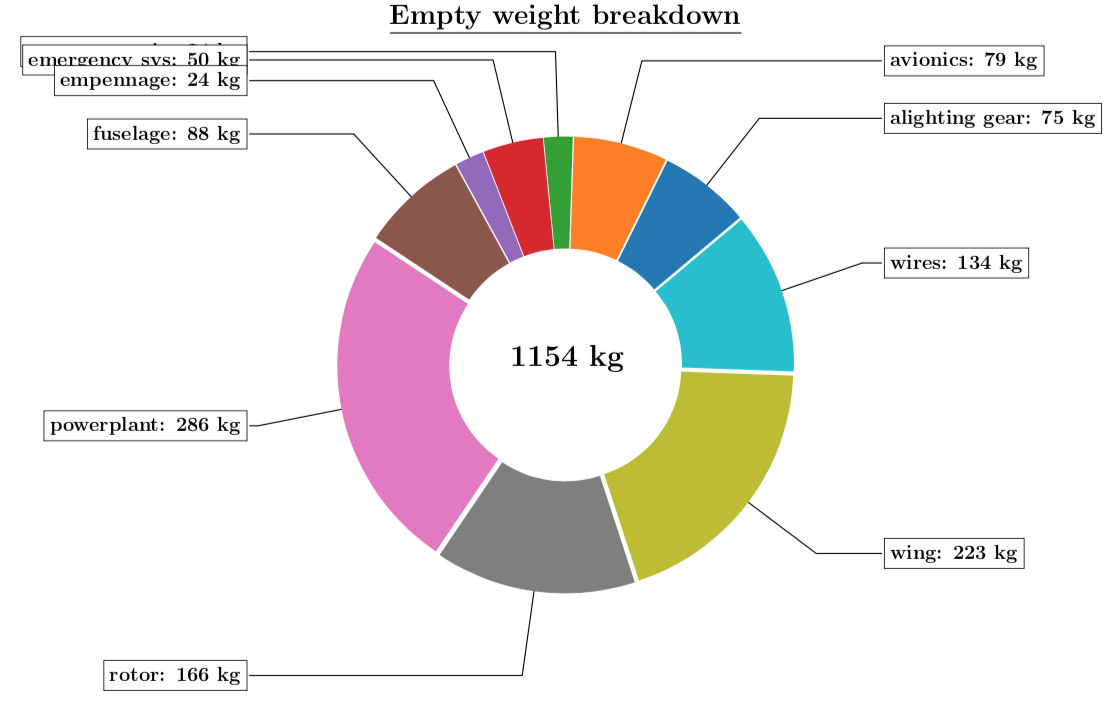
\includegraphics[width=0.45\textwidth]{images/pie7.png}}
     \caption{Pie charts generated by piethon.py postprocessor for a single design}
     \label{fig:pies}
\end{figure}

\item \textbf{Battery charge profile}: \hydra \spc features the ability to visualize the battery state of charge as a function of time along the mission profile. This postprocessor can be invoked with the command 
\begin{center}
\textbf{python3 Postprocessing/battery\_draw.py 10}
\end{center}
Here, 10 is the unique design ID for the sized vehicle that needs to be postprocessed. The resulting plot is stored in a PDF called \textbf{battery\_design\_10.pdf}, and shown in Fig.~\ref{fig:battery_profile}. The first subplot shows the estimated vehicle range for a ``perfect battery'' starting the mission at its theoretical maximum state of charge. The second subplot shows the same ``ideal battery'' charge, along with the estimated battery state of charge used in \hydra \spc for sizing the vehicle.

\begin{figure}
     \centering
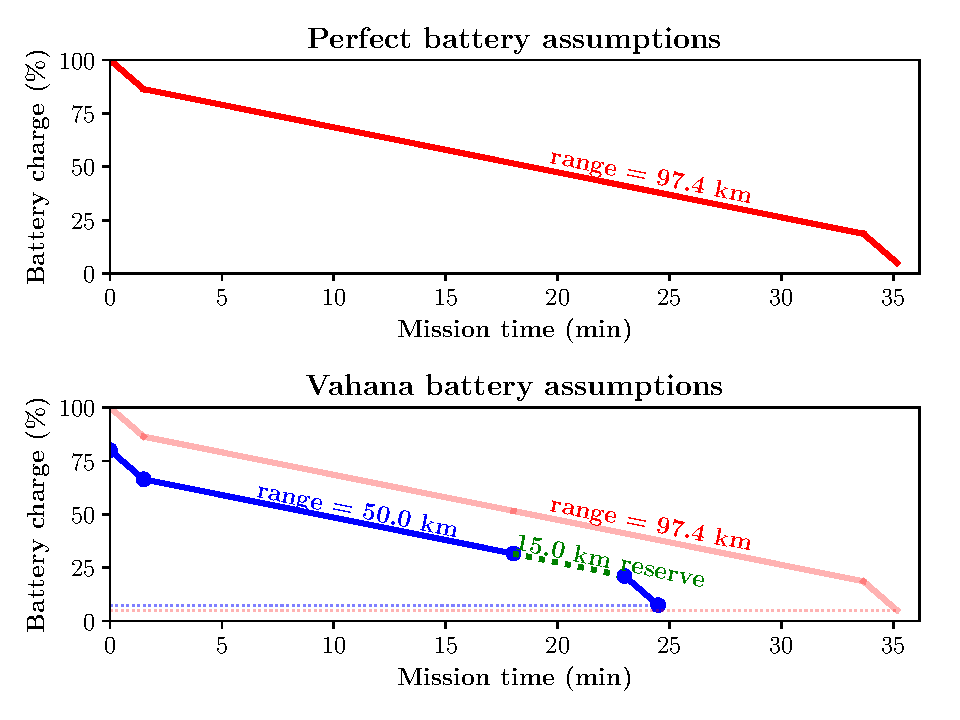
\includegraphics[width=0.9\textwidth]{images/battery_design_10.pdf}
\caption{Battery state of charge along mission profile}
\label{fig:battery_profile}
\end{figure}

\item \textbf{Vehicle performance}: To automatically generate the (approximate) power curve, payload-range and payload-endurance trade offs, \hydra \spc features a performance postprocessor that can be invoked as follows:
\begin{center}
\textbf{python3 Postprocessing/performance.py 28}
\end{center}
Here, 28 is the unique design identifier that will be analyzed at various airspeeds and longitudinal trim will be performed. The outputs from the postprocessor are shown in the following pages.

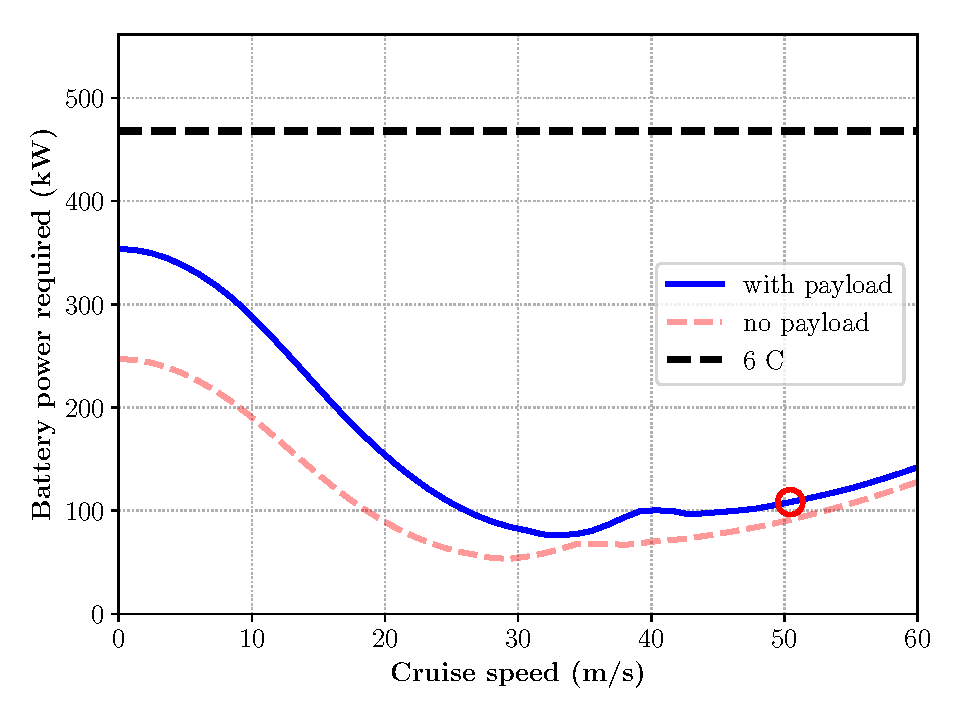
\includepdf[pages={1-}]{images/performance_design_28.pdf}

\item \textbf{Sensitivity analysis}: single and two-perturbation sensitivity studies can be launched using the following script:
\begin{center}
\textbf{python3 Postprocessing/sensitivity\_wrapper.py 32}
\end{center}
Here, 32 is the unique identifier for a converged vehicle design. The resulting plots from the sensitivity of the converged design to perturbations in target airspeed (for the same mission range) are shown in the first two plots. The next four plots show the effect of changing the cruise wing loading and aspect ratio on vehicle take-off mass, installed power, battery power and operating cost as contour plots, with carpet axes. The baseline design point is marked as a circle, and invalid designs are marked with a red cross (\red{$\times$}) inside a gray circle \textcolor{gray}{$\mathlarger{\circ}$}. The final two plots show the effect of changing the rotor hover blade loading and hover tip speed on take-off mass, installed power, battery mass and operating cost. These results are stored in a PDF named sensitivities\_design\_32.pdf.

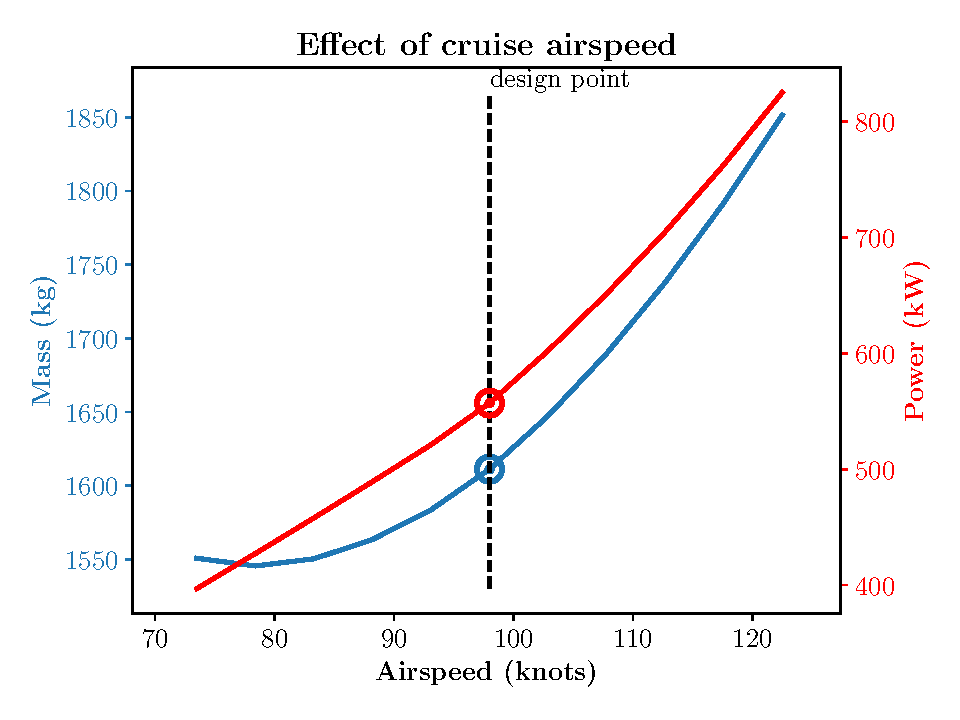
\includepdf[pages={1-}]{images/sensitivities_design_32.pdf}

\item \textbf{Optimization}: After running \textbf{xrun.py}, use the following commands to invoke sizing optimization:
\begin{flushleft}

\textbf{python3 process\_data.py}  \qquad  \#$\Rightarrow$ filter out invalid designs, rank\\
\textbf{python3 Postprocessing/optimize\_driver.py} \qquad \# serial mode\\
\textbf{mpirun -n 8 python3 Postprocessing/optimize\_driver.py} \# parallel
\end{flushleft}

This command launches two types of optimization: (a) gradient-based optimization (several threads), with several initial conditions based on valid designs identified by the \textbf{process\_data.py} command, and (b) differential evolution (first thread), with a latin-hypercube initial sampling. The optimized designs (generated by both methods) are aggregated and checked for uniqueness and validity. These unique designs are written to the file \textbf{optim\_summary.dat}, with the syntax identical to \textbf{summary.dat} and \textbf{best\_design.dat}. Additionally, the file \textbf{optim\_dvars\_summary.dat} shows the values of the design variables that yield the optimum design. After optimization is complete, the outputs/log/ folder will feature files with the pattern \textbf{optim\_log\_<XYZ>.yaml} and \textbf{optim\_log\_<XYZ>.txt}, with patterns similar to the regular output files of the same format. The process\_data.py command can be called with an additional argument `optim' as follows:
\begin{center}
\textbf{python3 process\_data.py optim}
\end{center}
This command sorts the various optimized unique designs in \textbf{optim\_summary.dat} from best to worst and writes the results in a file called \textbf{optim\_ranked.dat}.

\end{enumerate} 		% Postprocessing
\appendix
\section{Cantilever beam dynamics}

Consider an eVTOL wing with multiple electric motors and rotors mounted along the spar, shown in Fig.~\ref{fig:wing_diagram}. The wing structure is idealized as a cantilever beam with non-structural lumped masses placed along the span, shown in Fig.~\ref{fig:cantilever}. 

\begin{figure}[H]
     \centering
         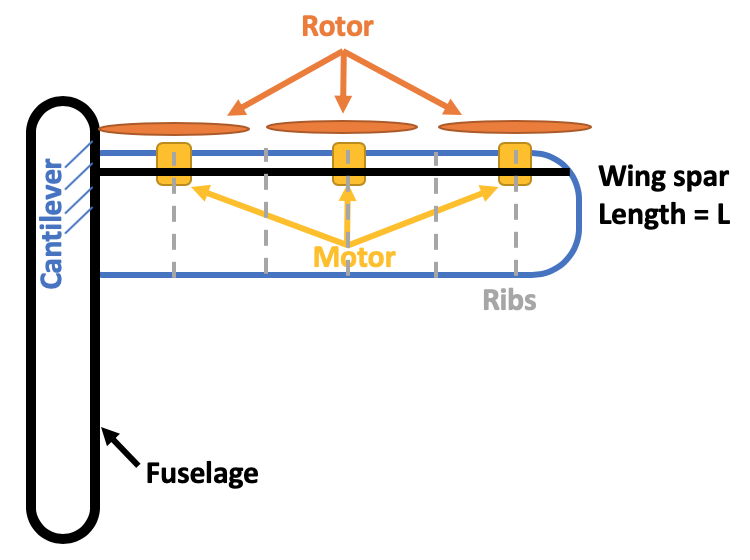
\includegraphics[width=0.7\textwidth]{images/wing_diagram.png}
        \caption{Rotor layout for an example eVTOL wing}
         \label{fig:wing_diagram}
\end{figure}

\begin{figure}[H]
         \centering
         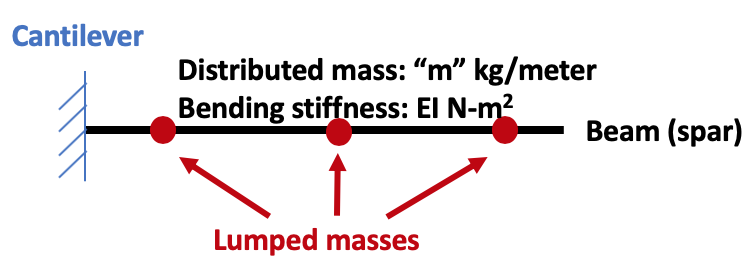
\includegraphics[width=0.7\textwidth]{images/cantilever.png}
        \caption{Idealization of eVTOL wing structure}
         \label{fig:cantilever}
\end{figure}

To expand the generality of the analysis, consider a tapered circular spar running along the length of the wing. The cross-section of the spar is shown in Fig.~\ref{fig:taper_beam}. The tube thickness is equal to $t$, and is uniform along the spar length. The radius of the circular cross-section varies from $r_1$ at the root of the beam to $r_2$ at the tip. The mass per unit span and bending stiffness of the spar is given by 
\begin{align*}
m(x) \quad &= \quad 2 \pi \rho r(x) t \\
EI_{yy}(x) \quad &= \quad E \pi r(x)^3 t
\end{align*}

\begin{figure}
\begin{center}
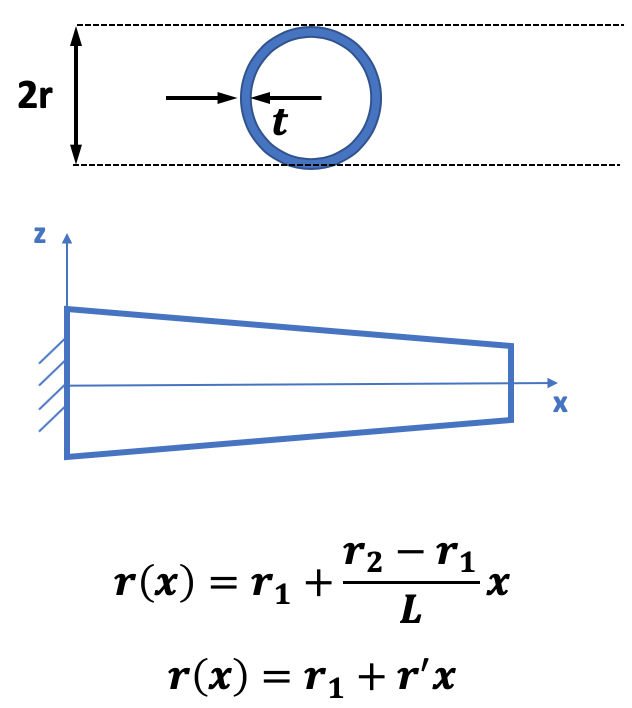
\includegraphics[width=0.45\textwidth]{images/taper_beam.png}
\vspace{-0.1cm}
\caption{Linearly tapered circular spar}
\label{fig:taper_beam}
\end{center}
\end{figure}

The first bending natural frequency is estimated using a Rayleigh-Ritz approximation, with a mode shape set by the static deflection of the cantilever due to a tip-load, i.e.,
\begin{equation}
w''(x) \quad = \quad P (L - x)
\end{equation}
Integrate twice along the span and apply the cantilever boundary condition to obtain the deflected bending slope as 
\begin{equation}
w'(x) \quad = \quad \frac{P}{E\pi t}\left[\frac{a_2}{r(x)^2} \spc+\spc \frac{a_1}{r(x)} \spc+\spc a_0\right]
\end{equation}
The constants are 
\begin{align*}
a_2 \quad =& \quad -\frac{L}{2r'} \spc-\spc \frac{r_1}{2{r'}^2} \\
a_1 \quad =& \quad -\frac{1}{{r'}^2} \\
a_0 \quad =& \quad \frac{L}{2r'r_1^2} \spc-\spc \frac{1}{2{r'}^2 r_1}
\end{align*}
Integrate the bending slope along the span to obtain the deflected mode shape as 
\begin{equation}
w(x) \quad = \quad \frac{P}{E\pi t}\left[b_0 \spc + \spc b_1 x \spc+\spc \frac{b_m}{r(x)} \spc+\spc b_l \log_e r(x)\right]
\end{equation}
The constants are 
\begin{align*}
b_0 \quad =& \quad -\frac{a_2}{r_1 r'} \spc-\spc \frac{a_1}{r'} \log_e(r_1)\\
b_1 \quad =& \quad a_0 \\
b_m \quad =& \quad -\frac{a_2}{r'}  \\
b_l \quad =& \quad \frac{a_1}{r'} 
\end{align*}
\subsection{Potential energy}
The maximum potential energy is given by 
\begin{equation*}
U \quad = \quad \frac{1}{2} \int_0^L \frac{P^2(L-x)^2}{EI_{yy}(x)} dx
\end{equation*}
Substitute for the bending stiffness to obtain 
\begin{equation*}
U \quad = \quad \frac{1}{2} \frac{P^2}{E\pi t} [A + B + C](\lambda) 
\end{equation*}
The term $\lambda$ is the spar taper ratio, given by 
\begin{equation}
\lambda \quad = \quad \frac{r_2}{r_1}
\end{equation}
The sum $A+B+C$ is well-represented by a cubic polynomial in $\lambda$ as 
\begin{equation*}
A+B+C\quad \approx \quad (1.6261 \spc - \spc 0.4826 \lambda \spc + \spc 2.1197 \lambda^2 \spc - \spc 0.5957 \lambda^3) \frac{1}{K^3}
\end{equation*}
The constant $K$ is the inverse of the spar aspect ratio, given by 
\begin{equation}
K \quad = \quad \frac{2 (\frac{t}{c})}{AR_{\rm wing}}
\end{equation}
Here, $\frac{t}{c}$ is the wing thickness to chord ratio, and $AR_{\rm wing}$ is the wing aspect ratio.

\subsection{Kinetic energy}
The maximum kinetic energy of the beam has contributions from three types of masses:
\begin{enumerate}
\item \textbf{Structural masses}: This term deals with the kinetic energy of the spar structure. This contribution to kinetic energy is 
\begin{equation*}
KE_{s} \quad = \quad \int_0^L \frac{1}{2} \spc 2 \pi r(x) t \rho \spc w(x)^2 \spc \omega_n^2 \spc dx \quad = \quad \frac{P^2}{E^2 \pi t} \rho \omega_n^2 (RHS)
\end{equation*}
The term $RHS$ is a function of the taper ratio $\lambda$, length $L$ and spar taper ratio inverse $K$ only. Further, the dependence on wing taper $\lambda$ can be approximated using a cubic polynomial in $\lambda$. Thus, the kinetic energy coefficient $RHS$ is approximated as 
\begin{equation*}
RHS \quad \approx \quad \frac{L^2}{K^5} (0.04823 \spc + \spc 0.269 \lambda \spc + \spc 0.15178 \lambda^2 \spc + \spc 0.36917 \lambda^3) 
\end{equation*}
\item \textbf{Non-structural distributed masses}: This term deals with the kinetic energy due to the skin and other components (e.g., wires) that do not contribute significantly to bending stiffness. The kinetic energy term is 
\begin{equation*}
KE_{\rm NS} \quad = \quad \int_0^L \frac{1}{2} \spc m_{\rm NS}(x)  \spc w(x)^2 \spc \omega_n^2 \spc dx 
\end{equation*}
The non-structural mass due to wing skin is given by 
\begin{equation*}
m_{\rm NS}(x) \quad = \quad \frac{2 M_{\rm NS}}{A (\frac{t}{c})} r(x) 
\end{equation*}
The term $\frac{M_{\rm NS}}{A}$ is the non-structural mass per unit plan-form area of the skin. Define an intermediate quantity $\beta$ given by 
\begin{equation*}
\beta \quad = \quad \frac{M_{\rm NS}}{A (\frac{t}{c})}
\end{equation*}
The expression for kinetic energy of non-structural masses simplifies to 
\begin{equation*}
KE_{\rm NS} \quad = \quad \beta \spc \frac{P^2 \omega_n^2}{E^2 \pi^2 t^2} \spc RHS
\end{equation*}
\item \textbf{Non-structural lumped mass}: This term refers to the kinetic energy of the electric motor/speed controller unit, rotor hubs and rotor blades. These discrete lumped masses are mounted along the wing spar, and the kinetic energy of these masses is given by 
\begin{equation*}
KE_{\rm lump} \quad = \quad \mathlarger{\mathlarger{\Sigma}}_i^{N_{\rm M}}\spc \frac{1}{2} \spc M_i \spc w(x_i)^2 \quad = \quad \frac{P^2 \omega_n^2}{E^2 \pi^2 t^2} \Delta RHS
\end{equation*}
The coefficient $\Delta RHS$ is 
\begin{equation*}
\Delta RHS \quad = \quad \mathlarger{\mathlarger{\Sigma}}_i^{N_{\rm M}} \frac{M_i}{2} \left[b_0 \spc + \spc b_1 x_i \spc + \spc b_l \log_e r(x_i) \spc + \spc \frac{b_m}{r(x_i)} \right]^2 
\end{equation*}
\end{enumerate}
\subsection{Frequency tuning}
The goal is to determine the spar mass by setting a target first natural frequency $\omega_n$ for the cantilever beam with distributed and lumped non-structural masses. Equating the maximum total kinetic energy and maximum potential energy for the first bending mode, we obtain
\begin{equation}
\frac{1}{2} \frac{P^2}{E^2 \pi t} \spc LHS \quad = \quad \omega_n^2 \left[\frac{P^2}{E^2 t} (RHS) \spc + \spc \frac{P^2}{E^2 \pi^2 t^2} \beta (RHS) \spc + \spc \frac{P^2}{E^2 \pi^2 t^2} \Delta RHS \right]
\end{equation}
Solve for spar thickness as 
\begin{equation*}
t \quad = \quad \left(\frac{E \pi}{2 \omega_n^2} LHS \spc - \spc \rho \pi RHS \right)^{-1} \left[\beta (RHS) \spc + \spc \Delta RHS \right]
\end{equation*}
The total spar mass is therefore 
\begin{equation}
M_{\rm spar} \quad = \quad \pi \rho \spc t (1 + \lambda) r_1 
\end{equation}

For validation of the Rayleigh-Ritz solution, several cases were evaluated with and without lumped non-structural masses. 

\subsection{Validation}
\subsubsection{Case 1: cantilever beam}
Consider a cantilever beam with a hollow circular cross-section of constant wall thickness, and the cross-section radius is linearly tapered from root to tip, with a taper ratio of $\lambda$ varying from 0.5 to 1.2. The beam length is 2.9 m, mean tube radius is 0.1411 m. The first bending natural frequency predictions from the Rayleigh-Ritz approximation are compared against a beam Finite Element Method analysis. These two frequencies are plotted in Fig.~\ref{fig:beam_freq1}. The Rayleigh-Ritz approximation exhibits about 2\% over-prediction, but otherwise captures the trends accurately. In this example, no non-structural masses were considered.

\begin{figure}
     \centering
	\subfigure[Natural frequency vs. taper ratio]{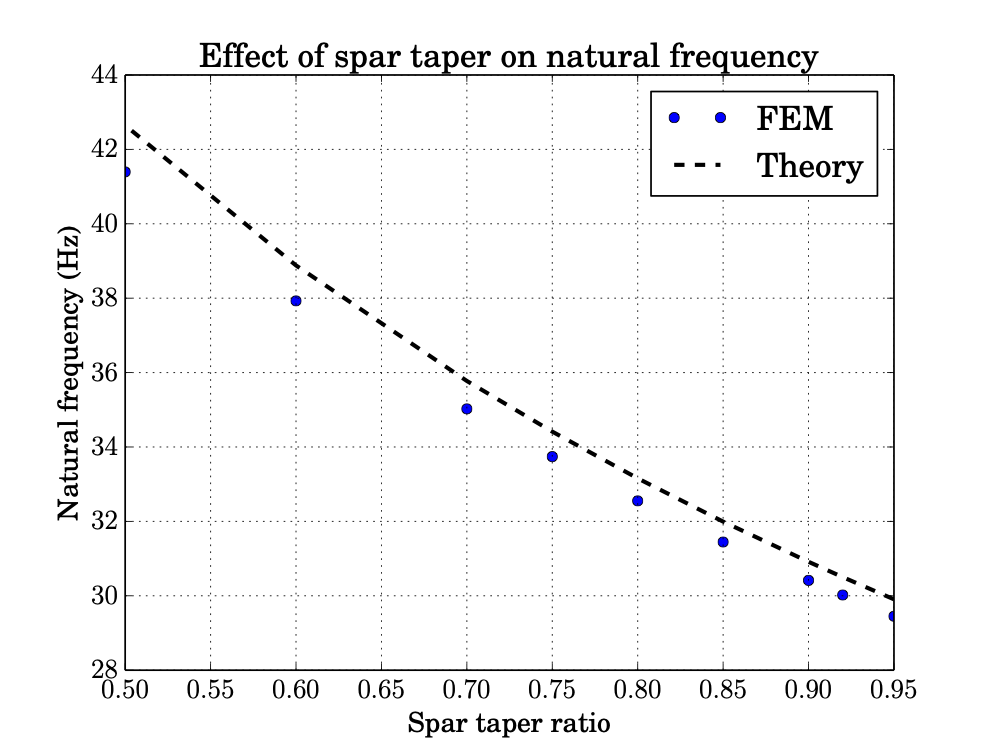
\includegraphics[width=0.45\textwidth]{images/beam_freq1b.png}}
	\subfigure[Rayleigh-Ritz vs. FEM]{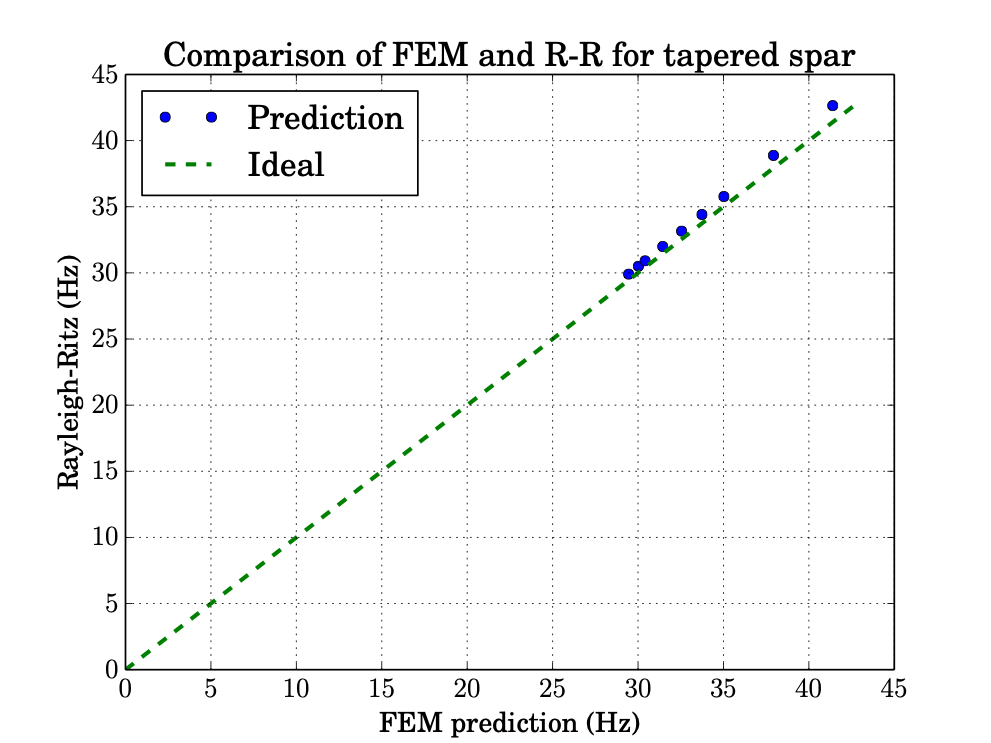
\includegraphics[width=0.45\textwidth]{images/beam_freq1.png}}
     \caption{Natural frequency: Rayleigh-Ritz vs. FEM predicted natural frequencies for a tapered cantilever beam}
     \label{fig:beam_freq1}
\end{figure}

\begin{figure}
     \centering
	\subfigure[Natural frequency vs. taper ratio]{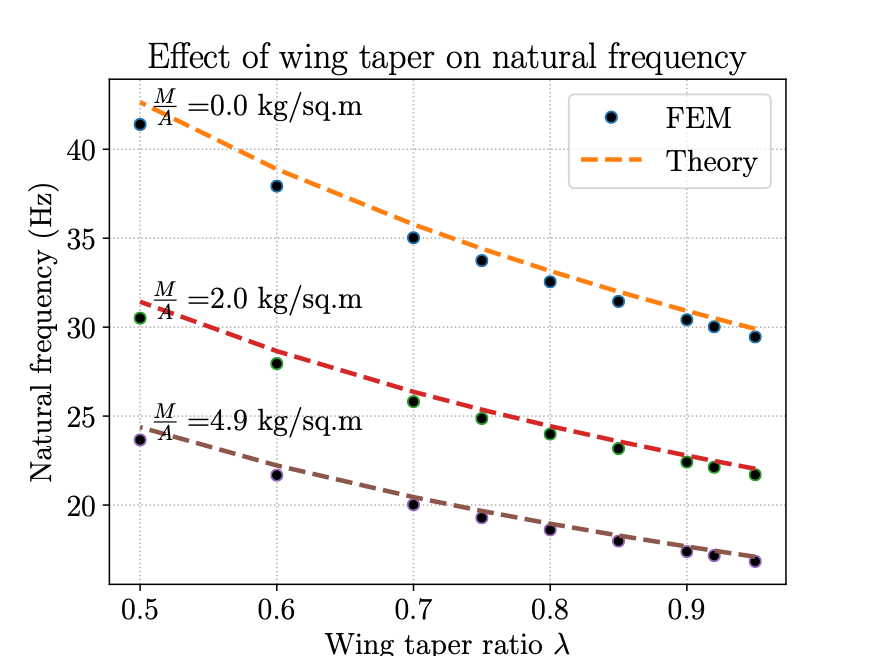
\includegraphics[width=0.45\textwidth]{images/beam_freq2b.png}}
	\subfigure[Rayleigh-Ritz vs. FEM]{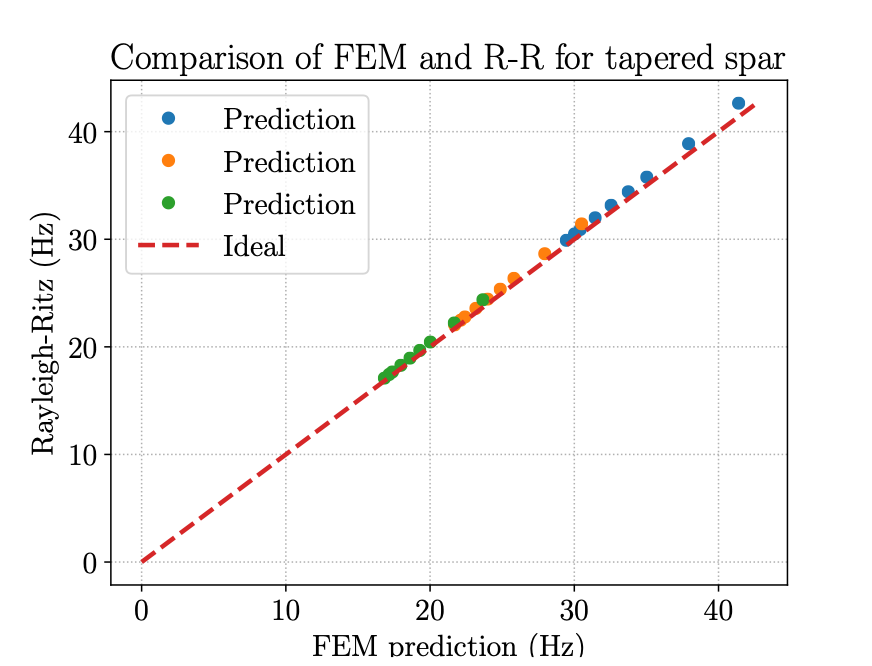
\includegraphics[width=0.45\textwidth]{images/beam_freq2.png}}
     \caption{Natural frequency: Rayleigh-Ritz vs. FEM for a tapered cantilever beam with distributed non-structural masses}
     \label{fig:beam_freq2}
\end{figure}

\subsubsection{Case 2: distributed non-structural mass}
This case is representative of an aircraft half-wing with skin, and no lumped masses. The non-structural masses are represented as a mass per unit area, i.e., $\large\frac{M}{A}$ kg/$m^2$. Three different values of the non-structural mass per unit wing area were evaluated: 0, 2.0 and 4.9 kg/m$^2$. The resulting natural frequencies were calculated from both Rayleigh-Ritz and FEM, and are plotted in Fig.~\ref{fig:beam_freq2}. Excellent agreement is obtained.

\subsubsection{Case 3: half-wing with lumped masses}
This case is representative of an eVTOL wing. The dimensions of the beam are the same as in the previous examples, and the distributed skin mass per unit area is 4.9 kg/m$^2$. Two lumped masses (21.3 kg, 27 kg) are placed along the beam at 0.5$L$ and $L$, respectively. The wing layout and natural frequencies are shown in Fig.~\ref{fig:beam_freq3}.

\begin{figure}
     \centering
	\subfigure[Layout of eVTOL wing]{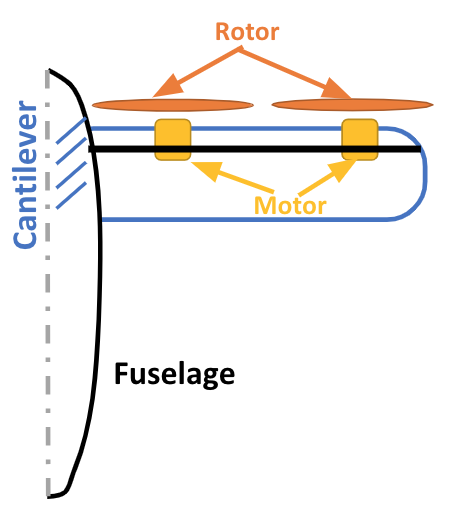
\includegraphics[width=0.3\textwidth]{images/wing_layout.png}}
	\subfigure[Rayleigh-Ritz vs. FEM]{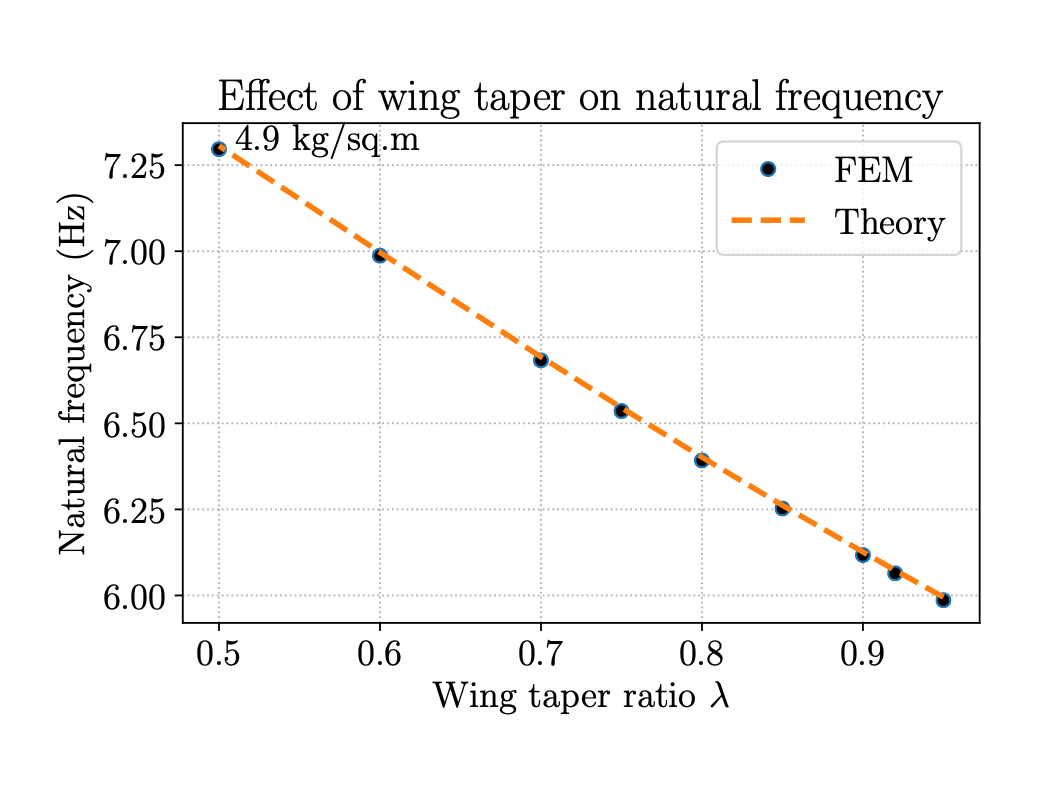
\includegraphics[width=0.45\textwidth]{images/beam_freq3b.png}}
     \caption{Natural frequency: Rayleigh-Ritz vs. FEM for an example eVTOL wing}
     \label{fig:beam_freq3}
\end{figure} 				% Appendix
%\section{What Next?}
This section details features of \hydra \spc that have not yet been documented, but may already exist in the code. It is a to-do list and reminder to document features.

\subsection{Rotor attributes}
\begin{enumerate}
\item Keyword recognition: tilting rotors 
\item Keyword recognition: ducts
\item Keyword recognition: symmetric/asymmetric booms
\item Auto-percolation of tilting attribute from wings (where applicable)
\item Dissimilar rotor groups on same wing, fuselage 
\end{enumerate}

\subsection{Wing and fuselage attributes}
\begin{enumerate}
\item Keyword recognition: tilt-wings vs. fixed 
\item Parametrically build FEM beam lattice representation around cabins 
\end{enumerate}

\subsection{Powerplant attributes}
\begin{enumerate}
\item Auto-addition of generator for turbine engine with electric transmission
\end{enumerate}

\subsection{Postprocessing}
\begin{enumerate}
\item Generation of vehicle top view with rotor/wing attachment, show components
\end{enumerate} 				% What next?

\renewcommand{\baselinestretch}{1}
\small\normalsize
\newpage
\bibliographystyle{ieeetr} 
\bibliography{references} 

\end{document}